\documentclass[a4paper,oneside,titlepage]{report}
%%%%%%%%%%%%%%%%%%%%%%%%%%%%%%%%%%%%%%%%%%%%%%%%%%%%%%%%%%%%%%%%%%%%%%%%%%%%%%%%%
%% Packages
%%%%%%%%%%%%%%%%%%%%%%%%%%%%%%%%%%%%%%%%%%%%%%%%%%%%%%%%%%%%%%%%%%%%%%%%%%%%%%%%%
\usepackage[english]{babel}
\usepackage{amsmath}
\usepackage{complexity}
\usepackage[T1]{fontenc}
\usepackage[utf8]{inputenc}
\usepackage[pdftex]{graphicx} %%Graphics in pdfLaTeX
\graphicspath{{images/}}
\usepackage{a4wide} %%Smaller margins, more text per page.
\usepackage{longtable} %%For tables that exceed a page width
\usepackage{pdflscape} %%Adds PDF support to the landscape environment of package
\usepackage{caption} %%Provides many ways to customise the captions in floating environments like figure and table
\usepackage{float} %%Improves the interface for defining floating objects such as figures and tables
\usepackage[tablegrid,nochapter]{vhistory} %%Vhistory simplifies the creation of a history of versions of a document
\usepackage[nottoc]{tocbibind} %%Automatically adds the bibliography and/or the index and/or the contents, etc., to the Table of Contents listing
\usepackage[toc,page]{appendix} %%The appendix package provides various ways of formatting the titles of appendice
\usepackage{pdfpages} %%This package simplifies the inclusion of external multi-page PDF documents in LATEX documents
\usepackage[rightcaption]{sidecap} %%Defines environments called SCfigure and SCtable (analogous to figure and table) to typeset captions sideways
\usepackage{cite} %%The package supports compressed, sorted lists of numerical citations, and also deals with various punctuation and other issues of representation, including comprehensive management of break points
\usepackage[]{acronym} %%This package ensures that all acronyms used in the text are spelled out in full at least once. It also provides an environment to build a list of acronyms used
\usepackage[pdftex,scale={.8,.8}]{geometry} %%The package provides an easy and flexible user interface to customize page layout, implementing auto-centering and auto-balancing mechanisms so that the users have only to give the least description for the page layout. For example, if you want to set each margin 2cm without header space, what you need is just \usepackage[margin=2cm,nohead]{geometry}.
\usepackage{layout} %%The package defines a command \layout, which will show a summary of the layout of the current document
\usepackage{subfigure} %%Provides support for the manipulation and reference of small or ‘sub’ figures and tables within a single figure or table environment.
\usepackage[toc]{glossaries} %%The glossaries package supports acronyms and multiple glossaries, and has provision for operation in several languages (using the facilities of either babel or polyglossia).
\usepackage[left,pagewise,modulo]{lineno} %%Adds line numbers to selected paragraphs with reference possible through the LATEX \ref and \pageref cross reference mechanism
\usepackage[pdftex,colorlinks=false,hidelinks,pdfstartview=FitV]{hyperref}%%The hyperref package is used to handle cross-referencing commands in LATEX to produce hypertext links in the document. 
\usepackage{metainfo}
\usepackage[pagestyles,raggedright]{titlesec}
\usepackage{etoolbox}
\usepackage{siunitx}
\usepackage{%
	array, %%An extended implementation of the array and tabular environments which extends the options for column formats, and provides "programmable" format specifications
	booktabs, %%The package enhances the quality of tables in LATEX, providing extra commands as well as behind-the-scenes optimisation
	dcolumn, %%
	rotating,
	shortvrb,
	units,
	url,
	lastpage,
	longtable,
	lscape,
	qtree,
	skmath,	
}
\usepackage{booktabs}
%%%%%%%%%%%%%%%%%%%%%%%%%%%%%%%%%%%%%%%%%%%%%%%%%%%%%%%%%%%%%%%%%%%%%%%%%%%%%%%%%
%% Listings
%%%%%%%%%%%%%%%%%%%%%%%%%%%%%%%%%%%%%%%%%%%%%%%%%%%%%%%%%%%%%%%%%%%%%%%%%%%%%%%%%
\usepackage{listings}
\usepackage{xcolor}
%\definecolor{pblue}{rgb}{0.13,0.13,1}
%\definecolor{pgreen}{rgb}{0,0.5,0}
%\definecolor{pred}{rgb}{0.9,0,0}
\definecolor{pgrey}{rgb}{0.46,0.45,0.48}
\definecolor{bggrey}{HTML}{E0E0E0}
\usepackage{inconsolata}
%\usepackage{bearmono}
% style for input files
\lstdefinestyle{inputfile}{%
  language=Fortran,
  basicstyle=\ttfamily,
  deletekeywords={in},
  frame=single,
  backgroundcolor=\color{gray!30}
}
% style for commands
\lstdefinestyle{command}{%
  language=bash,
  basicstyle=\ttfamily,
  frame=single,
  captionpos=b
}
\lstnewenvironment{inputfile}[1][]{%
  \renewcommand\lstlistingname{Input file}
  \lstset{style=inputfile,#1}}{}
\newcounter{inputfilelst}
\newcounter{commandlst}
\newcounter{tmp}

\definecolor{gray}{rgb}{0.4,0.4,0.4}
\definecolor{darkblue}{rgb}{0.0,0.0,0.6}
\definecolor{cyan}{rgb}{0.0,0.6,0.6}

\lstset{
  basicstyle=\ttfamily,
  columns=fullflexible,
  showstringspaces=false,
  commentstyle=\color{gray}\upshape
}

\lstdefinelanguage{XML}
{
  morestring=[b]",
  morestring=[s]{>}{<},
  morecomment=[s]{<?}{?>},
  stringstyle=\color{black},
  identifierstyle=\color{darkblue},
  keywordstyle=\color{cyan},
  morekeywords={xmlns,version,type},
  backgroundcolor=\color{gray!15}% list your attributes here
}

\makeatletter
% Environment for LaTeX listings; extension for auxiliar file: lll
\lstnewenvironment{command}[1][]{%
  \renewcommand\lstlistingname{Command}
  \setcounter{tmp}{\value{lstlisting}}
  \setcounter{lstlisting}{\value{commandlst}}
  \lstset{style=command,nolol,#1}
}{%
  \refstepcounter{commandlst}
  \addcontentsline{lll}{lstlisting}{\protect\numberline{\thelstlisting}\lst@@caption}%
  \setcounter{lstlisting}{\value{tmp}}
}
\makeatother

%%%%%%%%%%%%%%%%%%%%%%%%%%%%%%%%%%%%%%%%%%%%%%%%%%%%%%%%%%%%%%%%%%%%%%%%%%%%%%%%%
%% Examples etc
%%%%%%%%%%%%%%%%%%%%%%%%%%%%%%%%%%%%%%%%%%%%%%%%%%%%%%%%%%%%%%%%%%%%%%%%%%%%%%%%%
\usepackage{amsthm} 
\newtheoremstyle{example}{}{}{\itshape}{}{\bfseries}{\smallskip}{\newline}{}
\theoremstyle{example}
\newtheorem{example}{Example}



%%%%%%%%%%%%%%%%%%%%%%%%%%%%%%%%%%%%%%%%%%%%%%%%%%%%%%%%%%%%%%%%%%%%%%%%%%%%%%%%%
\setlength{\parindent}{0pt}
\setlength{\parskip}{.5\baselineskip}
%%%%%%%%%%%%%%%%%%%%%%%%%%%%%%%%%%%%%%%%%%%%%%%%%%%%%%%%%%%%%%%%%%%%%%%%%%%%%%%%%
%% Inserting the metadata
%%%%%%%%%%%%%%%%%%%%%%%%%%%%%%%%%%%%%%%%%%%%%%%%%%%%%%%%%%%%%%%%%%%%%%%%%%%%%%%%%
% % Metadaten des Dokumentes

\def\Company{}
\def\Institute{}
\def\Department{}

\def\BoldTitle{DUST User Manual}

\def\Subtitle{}
\def\Authors{ Davide Montagnani \\ Matteo Tugnoli \\ Federico Fonte \\ Alberto Savino \\ Alessandro Cocco} 


\title{\textbf{\BoldTitle}\\\Subtitle}
\author{\Authors \\ \\ \\ \Institute\\ \Department\\}
%\date{Milan, May 29\textsuperscript{th} 2018}

%%%%%%%%%%%%%%%%%%%%%%%%%%%%%%%%%%%%%%%%%%%%%%%%%%%%%%%%%%%%%%%%%%%%%%%%%%%%%%%%%
%% Creation of pdf information
%%%%%%%%%%%%%%%%%%%%%%%%%%%%%%%%%%%%%%%%%%%%%%%%%%%%%%%%%%%%%%%%%%%%%%%%%%%%%%%%%
\hypersetup{pdfinfo={
		Title={Title},
		Author={TR},
		Subject={Report}
	}}
%%%%%%%%%%%%%%%%%%%%%%%%%%%%%%%%%%%%%%%%%%%%%%%%%%%%%%%%%%%%%%%%%%%%%%%%%%%%%%%%%
%% Creating the frontpage
%%%%%%%%%%%%%%%%%%%%%%%%%%%%%%%%%%%%%%%%%%%%%%%%%%%%%%%%%%%%%%%%%%%%%%%%%%%%%%%%%
\AtBeginDocument{
	\maketitle
	\thispagestyle{empty}
}

%%%%%%%%%%%%%%%%%%%%%%%%%%%%%%%%%%%%%%%%%%%%%%%%%%%%%%%%%%%%%%%%%%%%%%%%%%%%%%%%%
%% Creation of the header
%%%%%%%%%%%%%%%%%%%%%%%%%%%%%%%%%%%%%%%%%%%%%%%%%%%%%%%%%%%%%%%%%%%%%%%%%%%%%%%%%
\patchcmd{\chapter}{plain}{short}{}{} %$ <-- the header on chapter 1
%%%%%%%%%%%%%%%%%%%%%%%%%%%%%%%%%%%%%%%%%%%%%%%%%%%%%%%%%%%%%%%%%%%%%%%%%%%%%%%%%
%% Creation of page-styles
%%%%%%%%%%%%%%%%%%%%%%%%%%%%%%%%%%%%%%%%%%%%%%%%%%%%%%%%%%%%%%%%%%%%%%%%%%%%%%%%%
\newpagestyle{long}{%
	\sethead[\thepage][][\chaptername\ \thechapter:\ \chaptertitle]{\chaptername\ \thechapter:\ \chaptertitle}{}{\thepage}
	\headrule
}

\newpagestyle{short}{%
	\sethead[\thepage][][]{}{}{\thepage}
	\headrule
}
%%%%%%%%%%%%%%%%%%%%%%%%%%%%%%%%%%%%%%%%%%%%%%%%%%%%%%%%%%%%%%%%%%%%%%%%%%%%%%%%%
%% CUSTOM COMMANDS
%%%%%%%%%%%%%%%%%%%%%%%%%%%%%%%%%%%%%%%%%%%%%%%%%%%%%%%%%%%%%%%%%%%%%%%%%%%%%%%%%
\newcommand{\param}[1]{\textbf{\texttt{#1}}}
\newcommand{\opt}[1]{\texttt{#1}}
\newcommand{\DUST}{DUST}

%%%%%%%%%%%%%%%%%%%%%%%%%%%%%%%%%%%%%%%%%%%%%%%%%%%%%%%%%%%%%%%%%%%%%%%%%%%%%%%%%
                                %% DOCUMENT
%%%%%%%%%%%%%%%%%%%%%%%%%%%%%%%%%%%%%%%%%%%%%%%%%%%%%%%%%%%%%%%%%%%%%%%%%%%%%%%%%
\begin{document}

\pagenumbering{roman}
\DeclareGraphicsExtensions{.pdf,.jpg,.png}
\pagestyle{short}

%%%%%%%%%%%%%%%%%%%%%%%%%%%%%%%%%%%%%%%%%%%%%%%%%%%%%%%%%%%%%%%%%%%%%%%%%%%%%%%%%
%% Version table insertion
%%%%%%%%%%%%%%%%%%%%%%%%%%%%%%%%%%%%%%%%%%%%%%%%%%%%%%%%%%%%%%%%%%%%%%%%%%%%%%%%%
% Versionstabelle.

\chapter*{Revision History}
\addcontentsline{toc}{chapter}{Revision History}
\begin{versionhistory}
	\vhEntry{1.0}{2018-09-14}{M.Tugnoli}{First partial version}
    \vhEntry{1.1}{2018-12-16}{M.Tugnoli}{Some updates to be consistent con DUST version 0.4.1, still partial}
    \vhEntry{1.2}{2018-12-19}{M.Tugnoli}{Updates of the contents to DUST version 0.5.0, added some other content, still partial}
    \vhEntry{1.3}{2019-2-12}{M.Tugnoli}{Added minor additional content}
    \vhEntry{1.4}{2019-3-12}{M.Tugnoli}{Updated contents to DUST version 0.5.3}
    \vhEntry{1.5}{2019-3-20}{M.Tugnoli}{Some additions on geometry}
    \vhEntry{1.6}{2019-3-26}{M.Tugnoli}{Updated contents to DUST version 0.5.5}
    \vhEntry{1.7}{2019-5-06}{M.Tugnoli}{Updated contents to DUST version 0.5.6}
    \vhEntry{1.8}{2019-5-10}{M.Tugnoli}{Updated contents to DUST version 0.5.7}
    \vhEntry{1.9}{2019-5-30}{M.Tugnoli}{Updated contents to DUST version 0.5.8}
    \vhEntry{1.10}{2019-6-4}{D.Montagnani}{Added pointwise geometry input}
    \vhEntry{1.11}{2019-6-11}{D.Montagnani}{Added examples of basic mesh generation}
    \vhEntry{1.12}{2019-7-25}{M.Tugnoli}{Updated contents to DUST version 0.5.10}
    \vhEntry{1.13}{2019-8-30}{D.Montagnani}{Added description and samples of files produced by DUST\_POST, added contents up to DUST version 0.5.11}
    \vhEntry{1.14}{2019-9-5}{M.Tugnoli}{Minor updates on postprocessing content and bodies of revolution}
    \vhEntry{1.15}{2019-10-21}{M.Tugnoli}{Updated contents to DUST version 0.5.13}
    \vhEntry{1.16}{2020-3-10}{M.Tugnoli}{Updated contents to DUST version 0.5.15}
    \vhEntry{1.17}{2020-8-21}{M.Tugnoli}{Updated contents to DUST version 0.5.17}
    \vhEntry{1.18}{2021-9-10}{A.Cocco, A.Savino}{Added contents on hinge surface}
    \vhEntry{1.19}{2022-3-3}{A.Cocco}{Added contents on non linear vortex lattice elements}
    \vhEntry{1.20}{2022-6-5}{A.Colli}{Added variable vortex rad, updated syntax and pressure and cp in postpro}
\end{versionhistory}


%\chapter*{Disclaimer}
The present document refers to the state of the code developed by
Politecnico di Milano for the collaboration with A3 Airbus at 
the present date. All the specifications herein contained are
subject to partial, substantial or complete modifications in the 
near future. The aim of the present document is to provide an early 
reference for the code usage and testing during the development 
phase and should not be considered in any form an official document
provided by Politecnico di Milano.  

\newpage
%%%%%%%%%%%%%%%%%%%%%%%%%%%%%%%%%%%%%%%%%%%%%%%%%%%%%%%%%%%%%%%%%%%%%%%%%%%%%%%%%
%% Table of contents
%%%%%%%%%%%%%%%%%%%%%%%%%%%%%%%%%%%%%%%%%%%%%%%%%%%%%%%%%%%%%%%%%%%%%%%%%%%%%%%%%
 \tableofcontents
 
 \vspace{1cm}

% % Wenn nicht im Inhaltsverzeichnis stehen soll:
\chapter*{Acronyms}
\addcontentsline{toc}{chapter}{Acronyms}

List of the acronyms employed in this document:

% % Wenns im Inhaltsverzeichnis stehen soll:
%\chapter{Liste der Abkürzungen}

% % Abkürzungen
% Das "ABCD" steht synonym für die längste Abkürzung in der Liste. Falls eine längere auftaucht, bitte anpassen.
\begin{acronym}
\acro{fmm}{Fast Multipol Method}
\acro{SP}{Surface (3D) Panel}
\acro{VL}{Vortex Lattice}
\acro{LL}{Lifting Line}
\acro{VP}{Vortex Particle}
\acro{VPM}{Vortex Particle Method}
\end{acronym}


\pagestyle{long}

\pagenumbering{arabic}
%%%%%%%%%%%%%%%%%%%%%%%%%%%%%%%%%%%%%%%%%%%%%%%%%%%%%%%%%%%%%%%%%%%%%%%%%%%%%%%%%
%% Inserting all the content
%%%%%%%%%%%%%%%%%%%%%%%%%%%%%%%%%%%%%%%%%%%%%%%%%%%%%%%%%%%%%%%%%%%%%%%%%%%%%%%%%
%\chapter{Introduction}
\label{ch:intro}

\section{Purpose}
\section{Document Conventions}
\section{Intended Audience and Reading Suggestions}
\section{Product Scope}
\section{References}


\chapter{Overall Description}
\label{Overall Description}

\section{Product Perspective}

\section{Product Functions}


\section{User Classes and Characteristics}


\section{Operating Environment}

\section{Design and Implementation Constraints}

\section{User Documentation}

\section{Assumptions and Dependencies}

\newpage




\chapter{External Interface Requirements}
\label{External Interface Requirements}

\section{User Interfaces}
\section{Hardware Interfaces}
\section{Software Interfaces}
\section{Communications Interfaces}


\chapter{System Features}
\label{System Features}

\section{System Feature 1}


\chapter{Other Nonfunctional Requirements}
\label{Other Nonfunctional Requirements}

\section{Performance Requirements}
\section{Safety Requirements}
\section{Security Requirements}
\section{Software Quality Attributes}
\section{Business Rules}

\chapter{Other Requirements}
\label{Other Requirements}

\begin{appendices}
\chapter{Glossary}
\chapter{Analysis Models}
\chapter{To Be Determined List}


\end{appendices}



\chapter{Introduction}

Dust is a flexible solution to simulate the aerodynamics of complex, 
non-conventional aircraft configuration.

It consists of three executables which are meant to perform preprocessing 
of the geometry, run the simulation in the desired condition and then postprocess 
the results obtained to gather the required meaningful data. 

\section{Workflow}
\label{sec:Workflow}

The most typical workflow with DUST is illustrated in figure \ref{fig:worflow}.  
The geometry of the solid bodies, in form of cgns mesh or parametric directive, 
must be provided to the preprocessor, which performs preliminary operations and 
generates a binary geometry file. 

Such file is provided, alongside the parameters for the simulation and the reference 
frames, to the solver, which executes the simulation and produces the complete results 
inside binary files. 

The produced results contain the complete solution obtained during the simulation, 
in terms of distribution of singularities on body surfaces and wake. However it is 
difficult to obtain condensed, meaningful data from such results.

For this reason it is possible to specify a variety of different analyses to be 
performed by the postprocessor, which employs the global results to generate a 
series of different meaningful results, from visualization and flow fields to 
loads and loads distribution, in different formats.

\begin{figure}[h]
\centering
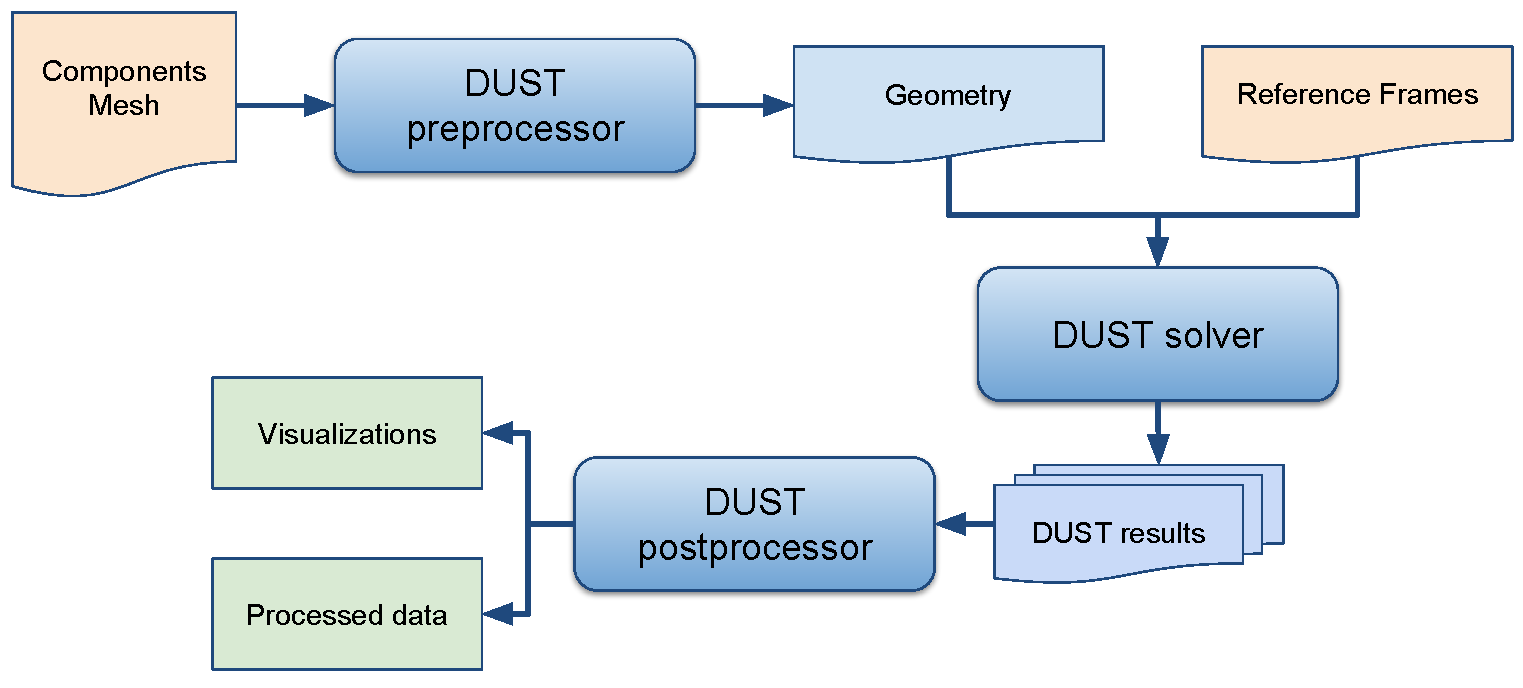
\includegraphics[width=\textwidth]{Workflow}
\caption{Description of the worflow with DUST}
\label{fig:worflow}
\end{figure}



\section{Input Files format}
\label{sec:InputFilesFormat}
All the input files, which are used to define parameters to the DUST executables, 
share the same flexible, free format text files structure.

The files are simple text files, without any requirement on the extension, 
however the extension \texttt{*.in} is recommended to distinguish the input 

files inside the case folders. The different executables automatically look 
for the input file \texttt{exe\_name.in} where they are invoked. 

An example of text input file is presented in file \ref{file:example}. 
input files employ loosely a Fortran syntax, and comprise of a series of 
keyword assignments.
The required keyword can generally be inserted in any order inside the input file, 
and should be written according to the following rules:
\begin{itemize}
\item Keywords use the snake_case naming convention
\item All the parameters assignments are written with an equal sign, i.e. keyword = value, 
for any kind of value.
\item Extra spaces and blank lines are ignored
\item Comments are introduced with an exclamation mark "!", and can be introduced 
at the beginning of a line, or after a valid keyword assignment.
\item Strings are introduced \emph{as they are}, without quotes, and will be 
automatically stripped of leading and trailing spaces
\item Integer and real numbers are introduced as usual, also with exponential notation
\item Logicals are introduced as "T" for true and "F" for false
\item Arrays can be introduced with the Fortran notation: contained between brackets 
and slashes and with elements separated by comas. 
\item Some keywords might be required to be contained inside a grouping keyword. 
It is a keyword which contains another set of keywords inside curly brackets. 
\end{itemize}

\begin{inputfile}[frame=single, caption={example input file}, label={file:example}]
! comments are introduced with an exclamation mark as in Fortran
example_string   = a_string
example_integer  = 59
example_real     = 67.84 !all comments even inline are ignored
example_logical  = T     !as well as all the extra spaces.

!empty lines are ignored
example_array = (/ 0.5, 2.3e-3, 5.67329/)

example_multiple = 1.3
example_multiple = 7.2 !some keywords can have multiple values

!some keyword can require to be grouped inside another grouping keyword
example_grouping = {
	grouped_var_int = 5 !indenting can be helpful, but is not required
    grouped_var_logical = F
}
\end{inputfile}

Regarding the number, position and compulsoriness of the keywords, depending on the keyword:
\begin{itemize}
\item Some keyword can be required and compulsory, some can be optional, in the sense that 
a default value is employed if the keyword is not defined, and also can be required only 
in specific cases, according choices made in other parameters (e.g. if the user requires 
a simulation to be restarted from file, should provide the file name, otherwise the file 
name keyword can be neglected)
\item Some keyword can be multiple: if the user should provide a list of a series of 
entities a keyword can be repeated several times
\item Some keyword, contrary to all the other, must be placed in precise relative 
position (before/after) another keyword, due to the strong correlation of the parameters.
\end{itemize}
All the details on the parameters of the single files will be provided in the description 
of each input file in the following chapters.

\section{Internal Binary Files format}
\label{sec:BynaryFilesFormat}
All the files that contain data, input geometry and results, which are not meant 
to be interpreted by the user but are only for internal use, are written in binary 
hdf5 format. 

The hdf5 format is a common opensource binary format which allows to store 
efficiently both in terms of size and I/O speed a variety of data in a single file. 

The standard extension for hdf5 files is \texttt{.h5} and, even if it is not 
compulsory, should be added to the binary filenames in the parameter when specified.

\section{Output Files format}
\label{sec:OutputFilesFormat}

As previously discussed in section \ref{sec:Workflow} the binary files results are 
not meant to be interpreted by the user (even if the use of applications as hdfView 
can give a brief insight on some results). The postprocessor can interpret those results 
and output processed data readily employable by the user.

Most of the postprocessed results can be obtained in Tecplot binary (\texttt{}) format, 
which is compact and convenient. However Tecplot is a proprietary software available only 
under licence. For this reason all the results can also be produced in the standard vtk 
format for visualizations (that can be opened by a variety of programs, e.g. paraview or 
visit) and formatted ascii files for line plots. 

Ascii files are also employed for analyses which output a single set of values (which are 
not meant to be plotted) and are convenient to be read inside automated execution loops. 

\chapter{Building DUST}
The building mechanism for DUST is currently under evolution in order to become 
more automated and reliable, however it is not in final configuration. 

For the current configuration refer to the file \texttt{INSTALL} in the root directory 
of the latest version of DUST.
\chapter{DUST Preprocessor}
\label{ch:Pre}

The DUST preprocessor is used to generate the geometrical components required to model 
the surfaces of the analysed body. It gathers the meshes of all the components required 
for the complete model, process them when necessary and generates all the parametrically 
specified components. 

The preprocessor is executed simply invoking the executable \texttt{dust\_pre} in the desired folder. 
The input file containing all the required informations for the execution of the preprocessor must be 
passed as argument to the command call. If not provided explicitly the preprocessor automatically 
tries to read the default input file \texttt{dust\_pre.in}.
\begin{command}[caption={Preprocessor command looking for input file \texttt{input\_file\_name.in}}]
  dust_pre input_file_name.in
\end{command}

\begin{command}[caption={Preprocessor command looking for 
default input file \texttt{dust\_pre.in}}, label={command:dus_pre_default}]
  dust_pre
\end{command}


\section{input file}
\label{sec:Pre_InputFile}

The input file of the preprocessor specifies the geometrical components required 
for the model, their name and the reference system to which they will be attached.

The format is the same as all the other input files, as already specified in 
section\ref{sec:InputFilesFormat}.

\begin{inputfile}[frame=single, caption={dust_pre.in}, label={file:dust_pre.in}]
comp_name = rotor
geo_file  = blade.in
ref_tag   = Hub01

comp_name = wing
geo_file  = wing.in
ref_tag   = Root01

tol_se_wing  = 0.001
inner_product_te = -0.5
file_name = ./geo_input.h5 
\end{inputfile}

An example of the preprocessor input file is presented in file 
\ref{file:dust_pre.in}, while the detailed parameters are:

\begin{itemize}
\item \param{comp_name}: \textit{required:} at least one. \textit{multiple:} yes. \textit{type} string.

This is the name assigned to the geometrical component. Will be mainly used by 
the user afterwards to specify postprocess analyses.

\item \param{geo_file}: \textit{required:} at least one. \textit{multiple:} yes. 
\textit{position:} must be after \param{comp_name}. \textit{type:} string. 

Indicates the auxiliary input file which must be provided with the details on the 
mesh of the component. It is a string with the path to the location of the file. 
In case of relative path the path is relative to the location in which the preprocessor was called.

\item \param{ref_tag}: \textit{required:} at least one. \textit{multiple:} yes. 
\textit{position:} must be after \param{geo_file}. \textit{type:} string

Provides a string tag which indicates the reference frame to which the geometrical 
component is attached. Must correspond to one of the reference frames that will be 
provided to the solver. 

\item \param{tol_se_wing}: \textit{required:} no. \textit{multiple:} no. 
\textit{default:} 0.001  \textit{type:} real.

Define the global tolerance at which the mesh node are merged to identify the open 
trailing edges. More details in section \ref{sec:TrailingEdge}.

\item \param{inner_product_te}: \textit{required:} no. \textit{multiple:} no. \textit{default:} -0.5 \textit{type:} real.

Define the global tolerance for the identification of trailing edges using the 
inner product of the normals.

\item \param{file_name}: \textit{required:} yes. \textit{multiple:} no. \textit{type:} string.

Define the name of the binary file which contains the geometry, to be used by the solver.
\end{itemize}

As discussed in section \ref{sec:BynaryFilesFormat} the file, being a DUST internal 
file is in binary hdf5 format. The use of the .h5 extension is not compulsory in a unix 
environment, but is recommended to distinguish internal binary files from input/output files 
in different formats.

\section{Geometry file}
The geometry file defines the parameters required to generate the geometry mesh of a component. 
Different components, with different component names and attached to different reference frames, 
can have the same geometry and hence use the same geometry file. A geometry file can be also use 
to define a parametric geometry, but details on that case will be described in section 
\ref{sec:Parametric_mesh_generation}. file \ref{file:geo_file.in} is an example of a 
geometry file for a non parametric geometry.

\begin{inputfile}[frame=single, caption={geo\_file.in}, label={file:geo_file.in}]
mesh_file = component-mesh.cgns
mesh_file_type = cgns
el_type = p

mesh_symmetry = F
symmetry_point  = (/0.0, 0.0, 0.0/)
symmetry_normal = (/0.0, 1.0, 0.0/)

mesh_mirror = F
mirror_point  = (/0.0, 0.0, 0.0/)
mirror_normal = (/1.0, 0.0, 0.0/)

tol_se_wing  = 0.001
inner_product_te = -0.5

proj_te = T
proj_te_dir = parallel
proj_te_vector = (/1.0, 0.0, 0.0/)
suppress_te = F

section_name = cgns_comp_1
section_name = cgns_comp_2

offset = (/0.0, 0.0, 0.0/)
scaling_factor = 1.0
\end{inputfile}

The detailed parameters of the geometry file are:
\begin{itemize}
\item \param{mesh_file}: \textit{required:} yes (if not parametric). \textit{multiple:} no. \textit{type:} string. 

name of the file containing the mesh.

\item \param{mesh_file_type}: \textit{required:} yes. \textit{multiple:} no. \textit{type:} string

type of the mesh. Valid options at the moment are \opt{cgns} for cgns, \opt{parametric} 
for parametrically generated meshes and \opt{basic} for ascii input meshes. 
The last is only for development purposes. 

\item \param{el_type}: \textit{required:} yes. \textit{multiple:} no. \textit{type:} character.

type of the elements of the mesh. \opt{p} stands for surface panels to model solid bodies, 
\opt{v} stands for vortex lattice elements used to model flat surfaces, \opt{l} stands for 
lifting lines used to produce a 1D model of a lifting surface (only for parametric input) and 
finally \opt{a} stands for actuator disk, to produce a simple model of a rotor (only for parametric input). 

\item \param{mesh\_symmetry} \textit{required:} no. \textit{multiple:} no. \textit{default:} false. \textit{type:} logical.

Choose to reflect the mesh around a point and a direction. Useful to produce full meshes out 
of symmetrical half models. Keeps both the original and the symmetrical part. 

\item \param{symmetry\_point}: \textit{required:} only if \param{mesh\_symmetry} is true. 
\textit{multiple:} no. \textit{default:} (0.0, 0.0, 0.0). \textit{type:} real array, length 3.

point around which to reflect the mesh.

\item \param{symmetry\_normal}: \textit{required:} only if \param{mesh\_symmetry} is true. 
\textit{multiple:} no. \textit{default:} (0.0, 1.0, 0.0). \textit{type:} real array, length 3.

Direction in which to reflect the mesh.

\item \param{mesh\_mirror} \textit{required:} no. \textit{multiple:} no. \textit{default:} false. \textit{type:} logical.

Choose to mirror the mesh around a point and a direction. Same as \param{mesh\_symmetry} 
but does not keep both the original, i.e. the mesh is not doubled.

\item \param{mirror\_point}: \textit{required:} only if \param{mesh\_mirror} is true. 
\textit{multiple:} no. \textit{default:} (0.0, 0.0, 0.0). \textit{type:} real array, length 3.

point around which to mirror the mesh.

\item \param{mirror\_normal}: \textit{required:} only if \param{mesh\_mirror} is true. 
\textit{multiple:} no. \textit{default:} (0.0, 1.0, 0.0). \textit{type:} real array, length 3.

Direction in which to mirror the mesh.

\item \param{tol_se_wing}: \textit{required:} no. \textit{multiple:} no. \textit{default:} 0.001 \textit{type:} real.

Tolerance in trailing edge merging of nodes. Override for the single component the value 
defined (or the default value) in the main input file to the preprocessor. 
Warning: the default value is not employed if the same parameter is defined (and not left default) in file \ref{file:dust_pre.in}. 

\item \param{inner_product_te}: \textit{required:} no. \textit{multiple:} no. \textit{default:} -0.5 \textit{type:} real
Tolerance for the identification of trailing edges using the inner product of the normals.
Override for the single component the value defined (or the default value) 
in the main input file to the preprocessor. Warning: the default value is not 
employed if the same parameter is defined (and not left default) in file \ref{file:dust_pre.in}. 

\item \param{proj_te}: \textit{required:} no. \textit{multiple:} no. \textit{default:} false \textit{type:} logical.

Force the projection of the trailing edge in a specific direction

\item \param{proj_te_dir}: \textit{required:} if \param{proj_te} is true. \textit{multiple:} no. \textit{type:} string.

Choose in which way to project the trailing edge. If it is \opt{parallel} the 
trailing edge direction will be forced in the direction given in \param{proj_te_vector}, 
while if it is \opt{normal} the trailing edge will be projected in a plane normal to \param{proj_te_vector}.

\item \param{proj_te_vector}: \textit{required:} if \param{proj_te} is true. 
\textit{multiple:} no. \textit{type:} real array, length 3.

vector to specify the direction declared in \param{proj_te_dir}

\item \param{suppress_te}: \textit{required:} no. \textit{multiple:} no. \textit{default:} false \textit{type:} logical.

Suppress the trailing edge from the component: even if a trailing edge is found, 
it is suppressed and the component will not release a wake from a trailing edge during the simulation.

\item \param{section_name} \textit{required:} no. \textit{multiple:} yes. \textit{type:} string 

To be used only with cgns meshes: specify only a subset of all the sections (geometrical components) 
available in the cgns file to be loaded and employed as geometry. 
If no \param{section_name} is specified, all the sections of the cgns file will be employed.

\item \param{offset} \textit{required:} no. \textit{multiple:} no. 
\textit{default:} (0.0, 0.0, 0.0) \textit{type:} real array, length 3.

offset to apply to the loaded points. Allows to move the coordinates of the loaded points of the vector specified. 

\item \param{scaling_factor} \textit{required:} no. \textit{multiple:} no. \textit{default:} 1.0 \textit{type:} real.

Scaling factor to apply to the loaded points. Allows to scale the coordinates of 
the loaded points of the specified factor.

offset and scaling are applied in the following order:
\begin{equation*}
\mathbf{r} = Scaling (\mathbf{r}_{loaded}+offset)
\end{equation*}
\end{itemize}

\subsection{Basic Mesh}
\label{subsec:Basic_Mesh}

The basic mesh input is an extremely simplified way to provide a surface mesh providing just the the 
position of points and point-element connectivity. 

When employing the basic way of input, the preprocessor expects two ascii files containing the points 
location and connectivity. If the parameter \param{mesh_file} was set to \opt{/path/to/mesh/} the 
preprocessor expects the point locations to be in \opt{/path/to/mesh/rr.dat} and the connectivity 
in \opt{/path/to/mesh/ee.dat} \footnote{Note that the preprocessor just add the suffix \opt{ee.dat} 
and \opt{rr.dat} to the basename, one can have different basic mesh files in a folder by giving them 
different prefixes and providing the path with the prefix to the input file, e.g 
\param{mesh_file} = \opt{/path/to/mesh/file_name\_} will look for \opt{/path/to/mesh/file_name\_rr.dat} 
and \opt{/path/to/mesh/file_name\_ee.dat}}

The points coordinates must be provided in the \opt{rr.dat} file as three floating point numbers 
each row, for a total of $n_p$ rows, where $n_p$ is the number of points in the mesh. The three 
numbers represent the $x, y$ and $z$ coordinates of each point (in the local reference frame).

The connectivity must be provided in the \opt{ee.dat} file as four integer numbers each row, for 
a total of $n_e$ rows, where $n_e$ is the total number of elements. Each row represents an element 
and the integers are the indices of the points forming the element, starting from one, in the order 
in which they were provided in the \opt{rr.dat} file.

Elements can be both quadrangular or triangular, in case of triangular elements use a 0 
as the fourth index. The order in which the points are listed in each element defines it 
normal, according to the right-handed screw rule. Neighbouring elements must not have opposing 
normals, and in three dimensional surface panels the normals direction should be outward from the body. 

\paragraph{Two examples of basic mesh generation via scripting.}
The MATLAB/OCTAVE scripts to generate the rectangular wing and the cylindrical ellipsoidal tank 
shown in figure \ref{fig:basic_components_example} are shown in this paragraph as an example of 
basic mesh generation along with the \opt{rr.dat}, \opt{ee.dat} files generated by the scripts 
to be read by DUST as input files.
\newline
\begin{figure}[h]
\centering
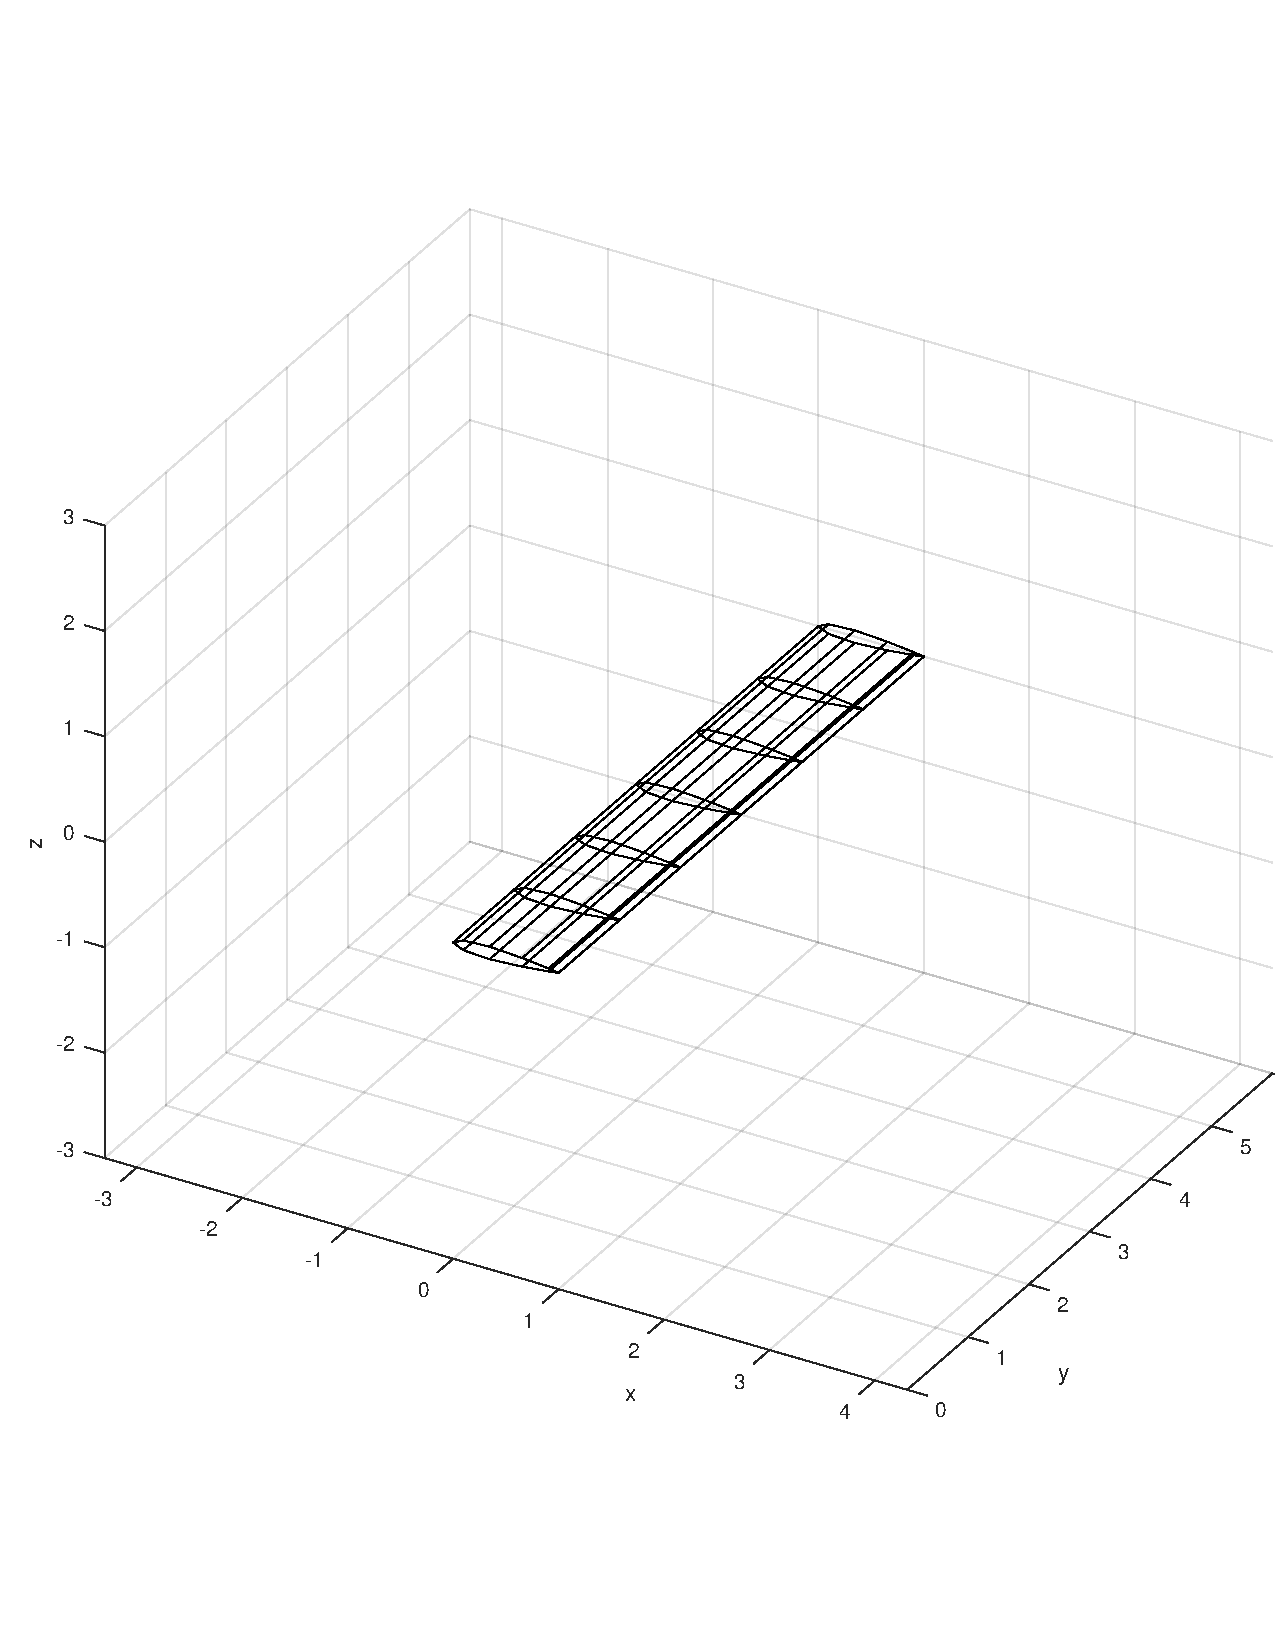
\includegraphics[width=.45\textwidth]{wing} \hspace{30pt}
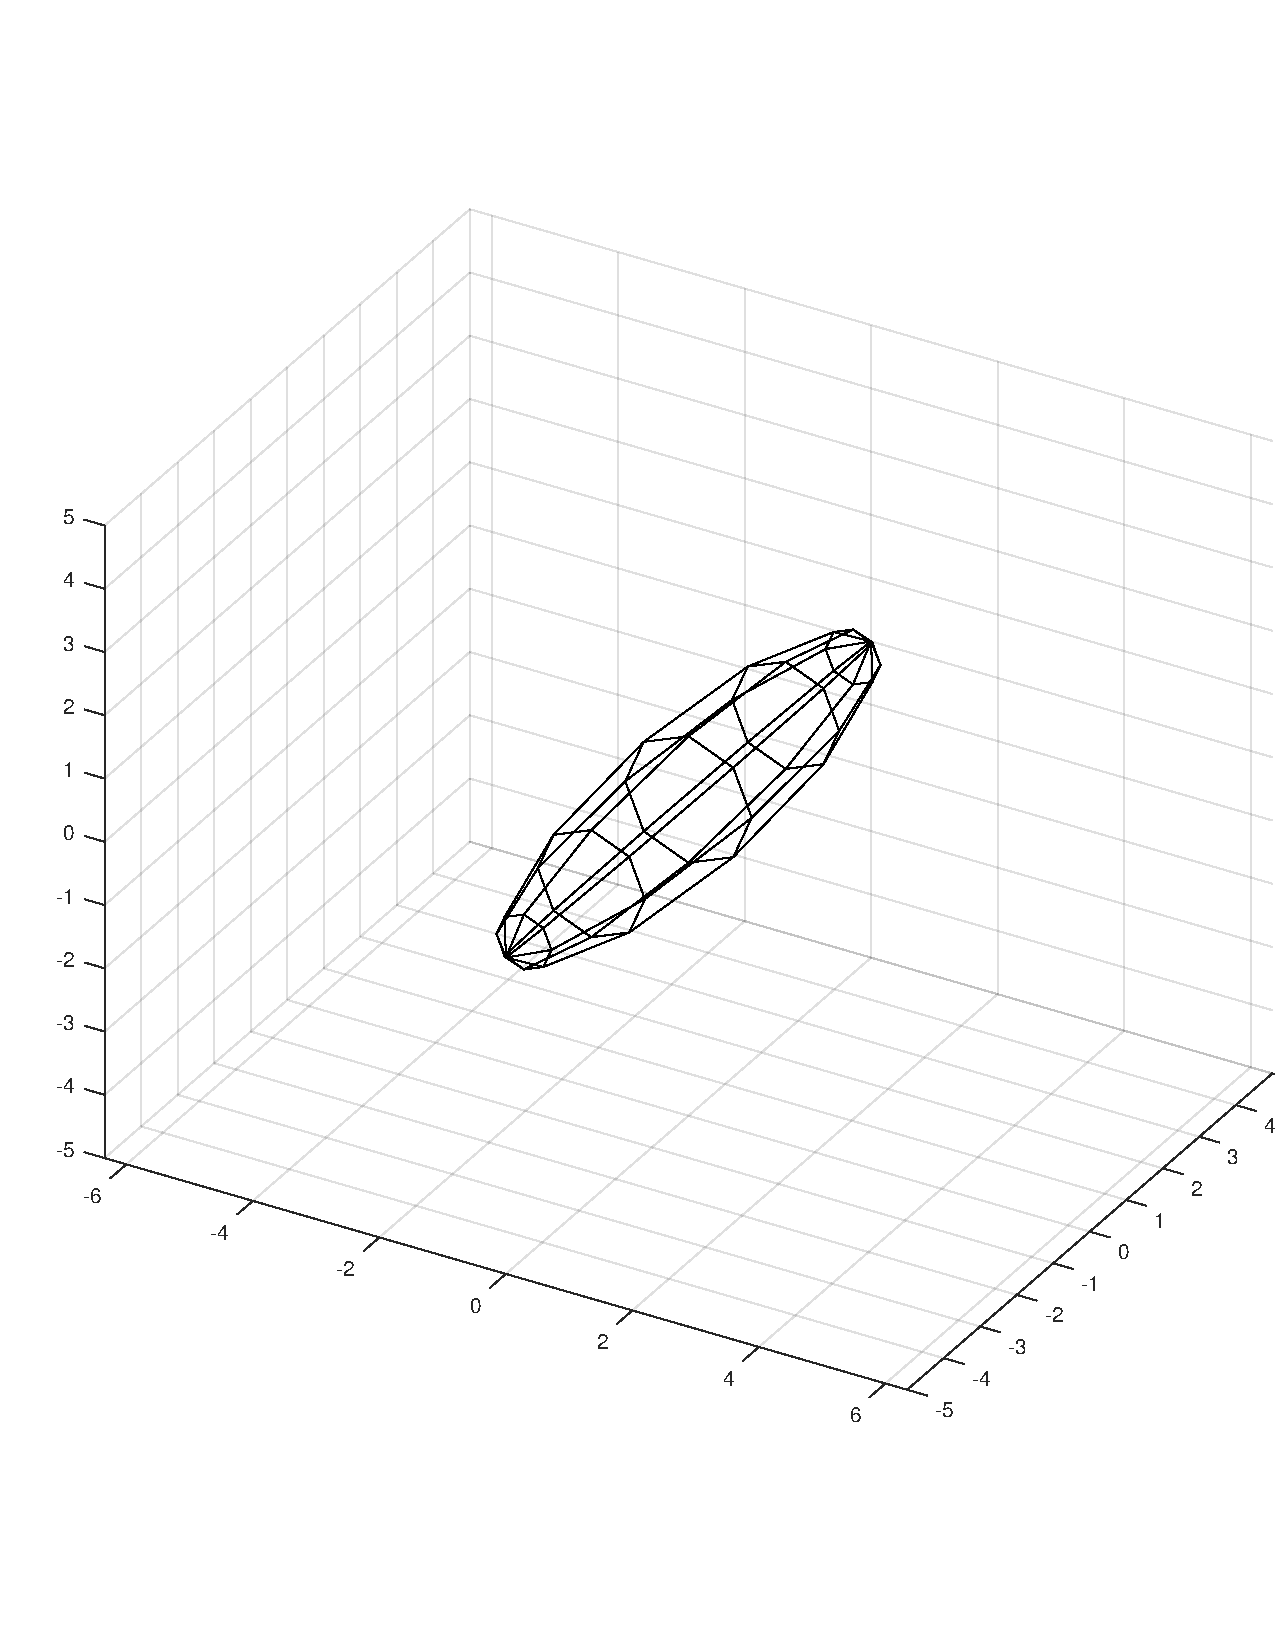
\includegraphics[width=.45\textwidth]{tank}
\caption{Components defined by means of basic mesh generations in the examples: wing and tank.}
\label{fig:basic_components_example}
\end{figure}
\newline
The following script \ref{file:wing_m} relies on the function \opt{setAirfoil4()} to define the two-dimensional 
airfoils and builds the basic input files for DUST of a rectangular wing with open tips.
\begin{inputfile}[frame=single, caption={\opt{wing.m}}, label={file:wing_m}]
% =========================================================================== %
% build the geometry and connectivity for a rectangular wing
% ( y-axis identifies the spanwise direction )
%
%  rr(3,n_points): array of the coordinates of the points of the surface
%  ee(4,n_elems ): array of the note-to-elem connectivity
% =========================================================================== %
clear all ; clc ; close all

% === params ===
chord      = 1.0 ;
span       = 6.0 ;
n_span_el  = 10  ;
n_chord_el = 5   ; % n_chord_el = n. elems on the chord

%> the tot. number of elems for a 3dpanel component ('p' in dust) is
n_elems = (n_span_el)*(2*n_chord_el) ;

%> the tot. number of points for a 3dpanel component ('p' in dust) is
n_points_per_sec = 2*n_chord_el+1 ;
n_points         = (n_span_el+1) * n_points_per_sec ;

%> vector of spanwise coord.s of the airfoil sections: uniform spacing, here
y_sec = linspace(0,span,(n_span_el+1)) ;

% === rr array ===
rr = zeros(n_points,3) ;

for i_sec = 1 : n_span_el+1

  %> define the 2d airfoil, NACA 4-digit airfoils, NACA-MPSS
  % setAirfoil ( M , P , SS , chord , n_chord_el , other parameters ... )
  [ x , z ] = setAirfoil4( 0 , 0 , 12 , chord , n_chord_el , ...
                           0.0 , 0.0 , 0.0 , 0.0 , 0 ) ; 
  %> update rr array
  rr(1+(i_sec-1)*n_points_per_sec:i_sec*n_points_per_sec,:) = ...
                                 [ x ; y_sec(i_sec)*ones(size(x)) ; z ]' ;
end

% === ee array ===
ee = zeros(n_elems,4) ; ie = 0 ;

for i_sec = 1 : n_span_el
  for i_p = 1 : n_points_per_sec-1

    ie = ie + 1 ;
    ee(ie,:) = [ i_sec   *n_points_per_sec+i_p   , ...
                 i_sec   *n_points_per_sec+i_p+1 , ...
                (i_sec-1)*n_points_per_sec+i_p+1 , ...
                (i_sec-1)*n_points_per_sec+i_p   ] ;
  end
end

% === check the connectivity with the Patch plot routine ===
% patch has rr,ee arrays as inputs --> easy way to check the rr,ee arrays
figure ; grid on ; axis equal
patch('Vertices',rr,'Faces',ee,'FaceColor','none')

% === save to .dat file in ascii format ===
%save('wing_rr.dat','rr','-ascii')
%save('wing_ee.dat','ee','-ascii')
dlmwrite('wing_rr.dat',rr, 'delimiter','\t')
dlmwrite('wing_ee.dat',ee, 'delimiter','\t')

\end{inputfile}
The files \ref{file:wing_rr} and \ref{file:wing_ee} are respectively the 
\opt{rr.dat} and \opt{ee.dat} files produced by the \opt{wing.m} script.

\begin{minipage}[]{0.48\textwidth}
 \begin{inputfile}[frame=single, caption={\opt{rr.dat} created by \opt{wing.m}}, label={file:wing_rr}]
    1.0000         0   -0.0013
    0.9045         0   -0.0139
    0.6545         0   -0.0409
    0.3455         0   -0.0596
    0.0955         0   -0.0460
         0         0         0
    0.0955         0    0.0460
    0.3455         0    0.0596
    0.6545         0    0.0409
    0.9045         0    0.0139
    1.0000         0    0.0013
    1.0000    1.0000   -0.0013
    0.9045    1.0000   -0.0139
    0.6545    1.0000   -0.0409
    0.3455    1.0000   -0.0596
    0.0955    1.0000   -0.0460
         0    1.0000         0
    0.0955    1.0000    0.0460
    0.3455    1.0000    0.0596
    0.6545    1.0000    0.0409
    0.9045    1.0000    0.0139
    1.0000    1.0000    0.0013
    1.0000    2.0000   -0.0013
    0.9045    2.0000   -0.0139
    0.6545    2.0000   -0.0409
    0.3455    2.0000   -0.0596
    0.0955    2.0000   -0.0460
         0    2.0000         0
    0.0955    2.0000    0.0460
    0.3455    2.0000    0.0596
    0.6545    2.0000    0.0409
    0.9045    2.0000    0.0139
    1.0000    2.0000    0.0013
    1.0000    3.0000   -0.0013
    0.9045    3.0000   -0.0139
   ...
    0.9045    6.0000    0.0139
    1.0000    6.0000    0.0013
 \end{inputfile}
\end{minipage} \hspace{10pt}
\begin{minipage}[]{0.48\textwidth}
 \begin{inputfile}[frame=single, caption={\opt{ee.dat} file created by \opt{wing.m}}, label={file:wing_ee}]
    12    13     2     1
    13    14     3     2
    14    15     4     3
    15    16     5     4
    16    17     6     5
    17    18     7     6
    18    19     8     7
    19    20     9     8
    20    21    10     9
    21    22    11    10
    23    24    13    12
    24    25    14    13
    25    26    15    14
    26    27    16    15
    27    28    17    16
    28    29    18    17
    29    30    19    18
    30    31    20    19
    31    32    21    20
    32    33    22    21
    34    35    24    23
    35    36    25    24
    36    37    26    25
    37    38    27    26
    38    39    28    27
    39    40    29    28
    40    41    30    29
    41    42    31    30
    42    43    32    31
   ...
    69    70    59    58
    70    71    60    59
    71    72    61    60
    72    73    62    61
    73    74    63    62
    74    75    64    63
    75    76    65    64
    76    77    66    65
 \end{inputfile}
\end{minipage}

 \noindent
The following script \ref{file:tank_m} builds the basic input files for DUST of a ellipsoidal tank with cylindrical sections.
\begin{inputfile}[frame=single, caption={\opt{tank.m}}, label={file:tank_m}]
% =========================================================================== %
% build the geometry and connectivity of a tank with ellipsoidal shape
% ( y-axis identifies the axial direction )
%
%  rr(3,n_points): array of the coordinates of the points of the surface
%  ee(4,n_elems ): array of the note-to-elem connectivity
%
%     /o----o--------o----o\
%    /_o----o--------o----o_\
%   o< -- . -- . -- . -- .  >o -- . -- axis
%    \ o----o--------o----o /
%     \o----o--------o----o/
%   sec.1   .2       .3   .4
% =========================================================================== %
clear all ; clc ; close all

% === params ===
a = 5.0 ; b = 1.0 ; % major and minor semi-axis of the cylindrical ellipsoid
n_axial_sec = 5   ; % n. cylindrical sections, excluding the tank extreme points
n_radial_el = 8   ; % n_chord_el = n. elems on the chord

%> the tot. number of elems for a 3dpanel component ('p' in dust) is
n_elems = n_radial_el * (n_axial_sec+1) ;

%> the tot. number of points for a 3dpanel component ('p' in dust) is
n_points_per_sec = n_radial_el ;
n_points = ...
  n_points_per_sec*n_axial_sec + 2 ; % + 2: for the extreme points

%> vector of spanwise coord. and radius of the tank sections
% here, ellipsoid with Chebychev spacing on the major axis
dth = pi/(n_axial_sec+2) ;
th_vec = linspace( pi-dth , dth , n_axial_sec ) ;
y_sec = a * cos(th_vec) ; 
r_sec = b * ( 1.0 - y_sec.^2 / a^2 ).^0.5 ;

%> extreme points y coord
y01 = - a ; y02 = a ;
 
% === rr array ===
rr = zeros(n_points,3) ; ir = 0 ;

for i_sec = 1 : n_axial_sec
  for i_p = 1 : n_points_per_sec

    %> update counter and find the th angle describing the polar coord
    ir = ir + 1 ;
    th = 2*pi*(i_p-1) / n_points_per_sec ;

    rr(ir,:) = [ r_sec(i_sec)*cos(th) , y_sec(i_sec) , r_sec(i_sec)*sin(th) ] ;

  end
end
%> update rr with the first and last point
rr = [ [ 0.0, -a, 0.0 ] ; rr(1:ir,:) ; [ 0.0, a, 0.0 ] ] ; 

% === ee array ===
ee = zeros(n_elems,4) ; ie = 0 ; % Initialisation to zero

%> first TRIA sector (last col remains equal to 0)
for i_p = 1 : n_points_per_sec

  ie = ie + 1 ;
  ee(ie,1:3) = [ 1 , 1+i_p , 1+mod(i_p,n_points_per_sec)+1 ] ;

end

%> inner QUAD sectors
for i_sec = 1 : n_axial_sec-1
  for i_p = 1 : n_points_per_sec

    ie = ie + 1 ;
    ee(ie,:) = int32([ 1+(i_sec-1)*n_points_per_sec+ i_p , ...
                 1+ i_sec   *n_points_per_sec+ i_p , ...
                 1+ i_sec   *n_points_per_sec+ mod(i_p,n_points_per_sec)+1 , ...
                 1+(i_sec-1)*n_points_per_sec+ mod(i_p,n_points_per_sec)+1 ]);
  end
end

%> first TRIA sector (last col remains equal to 0)
for i_p = 1 : n_points_per_sec

  ie = ie + 1 ;
  ee(ie,1:3) = int32([1+(n_axial_sec-1)*n_points_per_sec+i_p , ...
                n_points , ...
                1+(n_axial_sec-1)*n_points_per_sec+mod(i_p,n_points_per_sec)+1]);
                 
end

% === save to .dat file in ascii format (OCTAVE) ===
save('tank_rr.dat','rr','-ascii')
save('tank_ee.dat','ee','-ascii')
% === save to .dat file in ascii format (MATLAB) ===
dlmwrite('tank_rr.dat',rr, 'delimiter','\t')
dlmwrite('tank_ee.dat',ee, 'delimiter','\t')


% === check the connectivity with the Patch plot routine ===
% patch has rr,ee arrays as inputs --> easy way to check the rr,ee arrays
%> patch does not allow 0 indices in ee -> substitute 4th zero el with 3rd el
for ie = 1 : n_elems
 if ( ee(ie,4) == 0 ) ; ee(ie,4) = ee(ie,3) ; end 
end

figure ; grid on ; axis equal
patch('Vertices',rr,'Faces',ee,'FaceColor','none')

\end{inputfile}

\noindent
The files \ref{file:tank_rr} and \ref{file:tank_ee} are respectively the \opt{rr.dat} and \opt{ee.dat} 
files of the ellipsoidal tank, generated by the \opt{tank.m} script \ref{file:tank_m}.

\begin{minipage}[t]{0.48\textwidth}
 \begin{inputfile}[frame=single, caption={\opt{rr.dat} file created by \opt{tank.m}}, label={file:tank_rr}]
         0   -5.0000         0
    0.4339   -4.5048         0
    0.3068   -4.5048    0.3068
    0.0000   -4.5048    0.4339
   -0.3068   -4.5048    0.3068
   -0.4339   -4.5048    0.0000
   -0.3068   -4.5048   -0.3068
   -0.0000   -4.5048   -0.4339
    0.3068   -4.5048   -0.3068
    0.8467   -2.6602         0
    0.5987   -2.6602    0.5987
    0.0000   -2.6602    0.8467
   -0.5987   -2.6602    0.5987
   -0.8467   -2.6602    0.0000
   -0.5987   -2.6602   -0.5987
   -0.0000   -2.6602   -0.8467
    0.5987   -2.6602   -0.5987
    1.0000    0.0000         0
    0.7071    0.0000    0.7071
    0.0000    0.0000    1.0000
   -0.7071    0.0000    0.7071
   -1.0000    0.0000    0.0000
   -0.7071    0.0000   -0.7071
   -0.0000    0.0000   -1.0000
    0.7071    0.0000   -0.7071
    0.8467    2.6602         0
    0.5987    2.6602    0.5987
    0.0000    2.6602    0.8467
   -0.5987    2.6602    0.5987
   -0.8467    2.6602    0.0000
   -0.5987    2.6602   -0.5987
   -0.0000    2.6602   -0.8467
    0.5987    2.6602   -0.5987
    0.4339    4.5048         0
    0.3068    4.5048    0.3068
    0.0000    4.5048    0.4339
   -0.3068    4.5048    0.3068
   -0.4339    4.5048    0.0000
   -0.3068    4.5048   -0.3068
   -0.0000    4.5048   -0.4339
    0.3068    4.5048   -0.3068
         0    5.0000         0
 \end{inputfile}
\end{minipage} \hspace{10pt}
\begin{minipage}[t]{0.48\textwidth}
 \begin{inputfile}[frame=single, caption={\opt{ee.dat} file created by \opt{tank.m}}, label={file:tank_ee}]
     1     2     3     0
     1     3     4     0
     1     4     5     0
     1     5     6     0
     1     6     7     0
     1     7     8     0
     1     8     9     0
     1     9     2     0
     2    10    11     3
     3    11    12     4
     4    12    13     5
     5    13    14     6
     6    14    15     7
     7    15    16     8
     8    16    17     9
     9    17    10     2
    10    18    19    11
    11    19    20    12
    12    20    21    13
    13    21    22    14
    14    22    23    15
    15    23    24    16
    16    24    25    17
    17    25    18    10
    18    26    27    19
    19    27    28    20
    20    28    29    21
    21    29    30    22
    22    30    31    23
    23    31    32    24
    24    32    33    25
    25    33    26    18
    26    34    35    27
    27    35    36    28
    28    36    37    29
    29    37    38    30
    30    38    39    31
    31    39    40    32
    32    40    41    33
    33    41    34    26
    34    42    35     0
    35    42    36     0
    36    42    37     0
    37    42    38     0
    38    42    39     0
    39    42    40     0
    40    42    41     0
    41    42    34     0
 \end{inputfile}
\end{minipage} \hspace{10pt}



\section{Parametric mesh generation}
\label{sec:Parametric_mesh_generation}

The parametric mesh generation has the aim of allowing the generation of slender bodies, mainly wings, 
to be generated parametrically in the preprocessor with few directives, without resorting to an external mesh generator. 

To generate the parametric geometry a geometry input file to be referenced in the preprocessor input file 
\ref{file:dust_pre.in} is employed. The input file is similar to the geometry files for standard meshes described 
in file \ref{file:geo_file.in}


\subsection{Surface panels and vortex lattices}

\begin{inputfile}[frame=single, caption={paramtetric\_geo\_file.in}, label={file:parametric_geo_file.in}]
mesh_file_type = parametric
el_type = v

scaling_factor = 1.0
offset = (/0.0, 0.0, 0.0/)

airfoil_table_correction = T

mesh_symmetry = F
symmetry_point  = (/0.0, 0.0, 0.0/)
symmetry_normal = (/0.0, 1.0, 0.0/)

mesh_mirror = F
mirror_point  = (/0.0, 0.0, 0.0/)
mirror_normal = (/1.0, 0.0, 0.0/)

twist_linear_interpolation = F

starting_point = (/0.0,0.0865,0.0/)
reference_chord_fraction = 0.0

!mesh_flat = T

nelem_chord = 10
type_chord = cosineLE

! First section
chord = 1.0
twist = -1.0
airfoil_table = ./airfoils/naca0012.c81
airfoil = NACA0012

! First region
span = 0.5
sweep = 0.0
dihed = 0.0
nelem_span = 3 
type_span = uniform

! Second section
chord = 1.0
twist = 0.0
airfoil = interp

! Second region
span = 4.0
sweep = 10.0
dihed = 5.0
nelem_span = 10 
type_span = uniform

! Third section
chord = 0.5
twist =  0.0
airfoil_table = ./airfoils/naca0012.c81
airfoil = NACA0012

\end{inputfile}

The parametric geometry is obtained by connecting with a surface different planar sections. 
With the planar sections the user defines the shape of the section, the chord and the twist of the section. 
Then sections are connected by regions, with which the number of span panels, span, dihedral and sweep are defined. 
The user can define an arbitrary number $n_s$ of sections, which must then be connected with $n_s-1$ regions. 
A representation of sections and regions employed for the generation of a wing is presented in figure \ref{fig:parametric_wing}. 
The body is generated from the first section, starting from the specified starting point, and it is extruded along the y axis, 
with the x axis pointing from the leading edge towards the trailing edge and the z axis normal to the x-y plane. 
The type of geometry generated depends on the type of elements required. If surface panels are required the full 
three dimensional geometry will be generated, if vortex lattice elements are required only the flat, mean line 
surface will be generated and finally if lifting line elements are required only a one dimensional line will be generated. 
Finally the mirroring of the geometry introduced for user generated meshes is available also for parametric geometries.

All the detailed parameters of the geometry input file for parametric geometry are:
\begin{itemize}
\item \param{mesh_file_type}: \textit{required:} yes. \textit{multiple:} no. \textit{type:} string. 

Use \param{parametric} for parametric geometry.

\item \param{el_type}: \textit{required:} yes. \textit{multiple:} no. \textit{type:} character.

type of the elements of the mesh. \opt{p} stands for surface panels to model solid bodies, 
\opt{v} stands for vortex lattice elements used to model flat surfaces, \opt{l} 
stands for lifting lines used to produce a 1D model of a lifting surface. 

\item \param{offset} \textit{required:} no. \textit{multiple:} no. 
\textit{default:} (0.0, 0.0, 0.0) \textit{type:} real array, length 3.

offset to apply to the loaded points. Allows to move the coordinates of the loaded points of the vector specified. 

\item \param{scaling_factor} \textit{required:} no. \textit{multiple:} no. 
\textit{default:} 1.0 \textit{type:} real.

Scaling factor to apply to the loaded points. Allows to scale the coordinates of the loaded points of the specified factor.

offset and scaling are applied in the following order:
\begin{equation*}
\mathbf{r} = Scaling (\mathbf{r}_{loaded}+offset)
\end{equation*}


\item \param{airfoil_table_correction}: \textit{required:} yes. \textit{multiple:} no. \textit{type:} logical.

Require the viscous correction for \opt{v} elements by introducing the c81 aerodynamic tables. (Still experimental) 


\item \param{mesh\_symmetry} \textit{required:} no. \textit{multiple:} no. 
\textit{default:} false. \textit{type:} logical.

Choose to reflect the mesh around a point and a direction. Useful to produce full meshes out of symmetrical half models. 
Keeps both the original and the symmetrical part. 

\item \param{symmetry\_point}: \textit{required:} only if \param{mesh\_reflection} is true. \textit{multiple:} no. 
\textit{default:} (0.0, 0.0, 0.0). \textit{type:} real array, length 3.

point around which to reflect the mesh.

\item \param{symmetry\_normal}: \textit{required:} only if \param{mesh\_reflection} is true. \textit{multiple:} no. 
\textit{default:} (0.0, 1.0, 0.0). \textit{type:} real array, length 3.

Direction in which to reflect the mesh.

\item \param{mesh\_mirror} \textit{required:} no. \textit{multiple:} no. \textit{default:} false. \textit{type:} logical.

Choose to mirror the mesh around a point and a direction. Same as \param{mesh\_symmetry},
but does not keep both the original, i.e. the mesh is not doubled.

\item \param{mirror\_point}:  \textit{required:} only if \param{mesh\_reflection} is true. \textit{multiple:} no. 
\textit{default:} (0.0, 0.0, 0.0). \textit{type:} real array, length 3.

point around which to mirror the mesh.

\item \param{mirror\_normal}: \textit{required:} only if \param{mesh\_reflection} is true. \textit{multiple:} no. 
\textit{default:} (0.0, 1.0, 0.0). \textit{type:} real array, length 3.

Direction in which to mirror the mesh.

\item \param{twist\_linear\_interpolation} \textit{required:} no. 
\textit{multiple:} no. \textit{default:} false. \textit{type:} logical.

Choose to apply linear interpolation to the twist angle, instead of interpolating the point coordinates between two neighboring sections defined in the input file.

\item \param{starting\_point} \textit{required:} no. \textit{multiple:} no. 
\textit{default:} (/ 0.0, 0.0, 0.0 /) \textit{type:} real array, length 3.

point in the local reference frame in which to start extruding the parametric geometry.

\item \param{reference\_chod\_fraction} \textit{required:} no. 
\textit{multiple:} no. \textit{default:} 0.0 \textit{type:} real

Fraction of the chord at which to place the axis which will be rotated of the sweep and dihedral angles, and 
around which airfoils are twisted. 

\item \param{mesh\_flat} \textit{required:} no. \textit{multiple:} no. 
\textit{default:} true \textit{type:} logical

Used only in case of lifting lines (\opt{l}) elements. If enabled instead of generating lifting lies 
actually twisted according to the input twist, but rather a flat surface with only the normal vectors twisted 
according to the input twist. 

\item \param{nelem\_chord} \textit{required:} yes, if parametric. \textit{multiple:} no. \textit{type:} integer.

Number of elements in chord direction. Note: if the elements are vortex lattice $nelem\_chord$ 
elements will be generated, while in case of surface panels $2nelem\_chord$ elements will be produced, 
$nelem\_chord$ on the lower and $nelem\_chord$ on the upper side. In case of lifting lines this parameter is ignored.

\item \param{type\_chord} \textit{required:} no. \textit{multiple:} no. 
\textit{default:} uniform \textit{type:} string.

Type of subdivision in the chord-wise direction. Can be \opt{uniform} for a uniform distribution (suggested for vortex lattices), 
\opt{cosine} for a cosine distribution, refined both on the leading and trailing edge, 
\opt{cosineLE} for a half cosine refined only on leading edge (suggested for surface panels) or \opt{cosineTE} for a +
half cosine refined only on the trailing edge. 

\item \param{chord} \textit{required:} at least 2. \textit{multiple:} yes. \textit{type:} real.

Defines a section, by its chord length

\item \param{twist} \textit{required} in same number as \param{chord}. \textit{multiple} yes. \textit{type:} real.

Angle of twist, in degrees, of the airfoil section.

\item \param{airfoil}/\param{airfoil\_table} \textit{required:} in same number as 
\param{chord}. \textit{multiple:} yes. \textit{type:} string.

Airfoil of the section. There are different ways to define an airfoil. It can be defined by the user as a 
series of points, and so \param{airfoil} must be the path to a .dat file (the extension is mandatory) 
containing the two dimensional coordinates of an airfoil; the file must have in the first line an integer 
representing the number of points provided, followed by the coordinates of each point on separate lines. 
It can also be an analytical NACA profile, and so must be provided as a 
NACAXXXX string (at the moment only 4 digits and some 5 digits are implemented). 

In case of lifting lines or when \param{airfoil\_table\_correction} is true on the vortex lattice, to mark 
the difference the \param{airfoil\_table} must be employed, and it refers to the path to the corresponding c81 lookup table. 

Optionally in the \param{airfoil} or \param{airfoil\_table} parameter it is possible to specify the option 
\opt{interp}. In this case the airfoil (airfoil section, mean line, section defined from file or c81 lookup 
table according to the type of elements) in the section will be linearly interpolated among the pair of 
explicitly specified airfoils in which the section is contained. 

\item \param{span} \textit{required:} at least one, in same number as \param{chord}-1 \textit{multiple:} yes. \textit{type:} real.

Define the span length of the region between two sections.  

\item \param{sweep} \textit{required:} in same number as \param{span} \textit{multiple:} yes. \textit{type:} real.

Angle of sweep of the region, positive if swept backwards (towards positive x).

\item \param{dihed} \textit{required:} in same number as \param{span} \textit{multiple:} yes. \textit{type:} real.

Angle of dihedral of the region, positive if rotated upwards (towards positive z).

\item \param{nelem\_span} \textit{required:} in same number as \param{span} \textit{multiple:} yes. \textit{type:} integer.

Number of elements in the spanwise direction, in the single region.

\item \param{type\_span} \textit{required:} in same number as \param{span} \textit{multiple:} yes. \textit{type:} string.

type of refinement of the elements in the spanwise direction. As for the chordwise direction, 
the options are \opt{uniform} for a uniform distribution, \opt{cosine} for a cosine refinement both 
inboard and outboard, and \opt{cosine_ib} and \opt{cosine_ob} for half cosine refinement only inboard or outboard. 
  
\end{itemize}

%TODO: actuator disk?

The concept of sections and regions is illustrated in figure \ref{fig:parametric_wing}. 
Furthermore an example to understand the geometrical role of the parameters in the input file is presented 
in file \ref{file:parametric_example_file.in} and figure \ref{fig:parametric_sections}.

\begin{figure}[h]
\centering
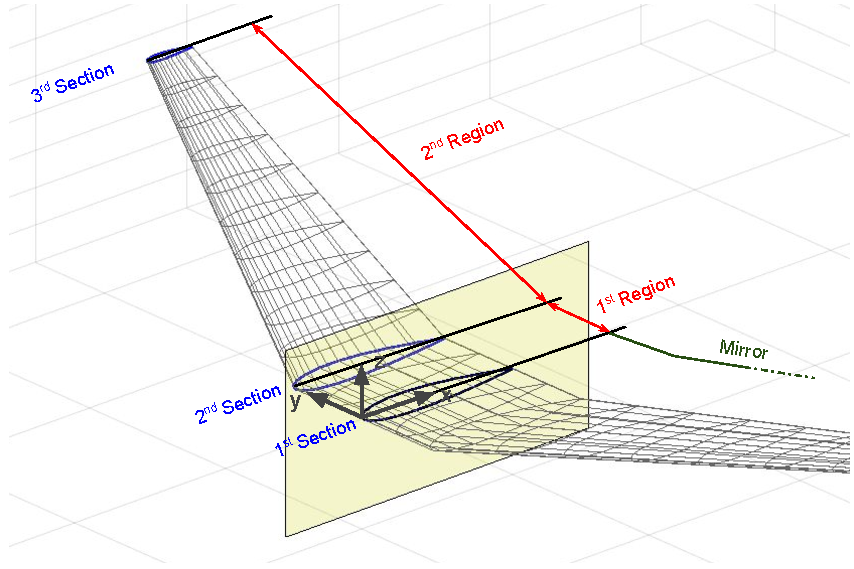
\includegraphics[width=.7\textwidth]{parametric_wing}
\caption{Sections and regions in parametric wing generation}
\label{fig:parametric_wing}
\end{figure}

When generating the parametric geometry, the slender body is generated starting from the \param{starting\_point} 
and then develops in the y direction (in the local reference frame of the component), 
with deviations induced by the various angles used as input. 

From the \param{starting\_point} a segmented reference line is created, in blue in figure \ref{fig:parametric_sections}. 
Each segment, which creates a region as in figure \ref{fig:parametric_wing}, is created from the previous node, 
is long \param{span} and is angled from the local component y direction of \param{dihed} dihedral angle with respect 
to the horizontal plane (rotating around the local x axis, positive upward, red in the figure) and of \param{sweep} 
angle with respect to the vertical plane (rotating around the local z axis, positive backward towards x, green in figure). 

Then on each node the airfoil section is applied, 2 dimensional for surface panels (as in figure) mono dimensional for 
vortex lattices (lifting lines will be discussed afterwards). 
The section is collocated so that the reference line passes through a certain \param{reference\_chord\_fraction} 
of the airfoil chord. Then the section is rotated around such point of a \param{twist} angle 
(around the component local y axis, positive when creating a positive pitch to the airfoils, in magenta in the figure). 

Finally all the sections are connected with the appropriate number of elements, as shown in figure \ref{fig:parametric_wing}.

\begin{figure}[h]
\centering
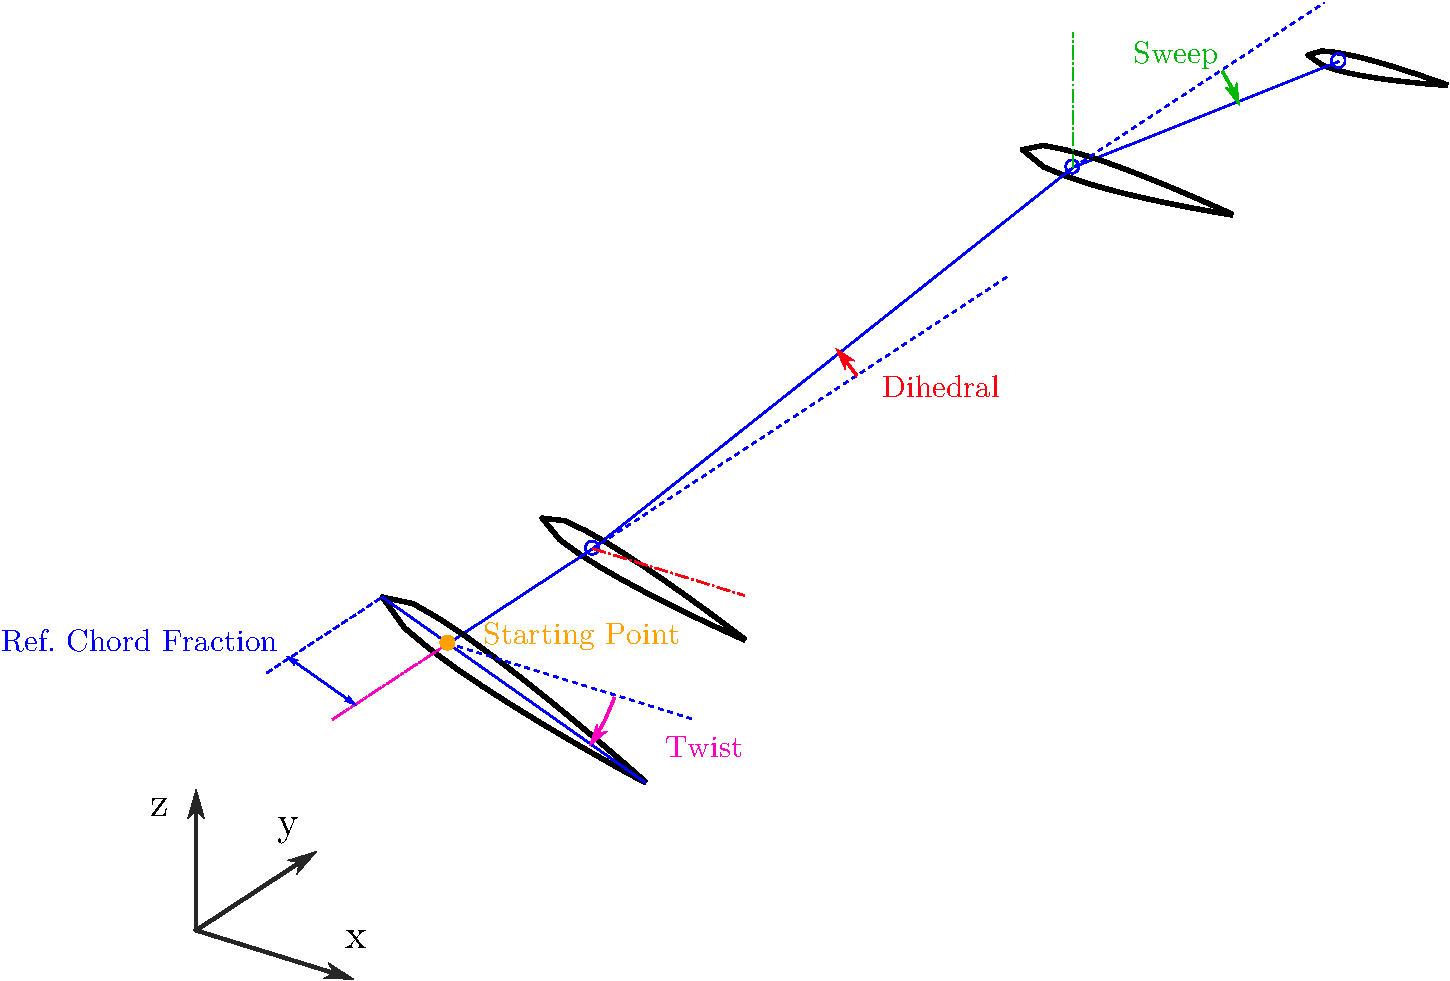
\includegraphics[width=.7\textwidth]{parametric_sections}
\caption{Generation logic of the geometry of parametric elements, generated from input file \ref{file:parametric_example_file.in}}
\label{fig:parametric_sections}
\end{figure}

\begin{inputfile}[frame=single, caption={Parametric geometry for figure \ref{fig:parametric_sections}}, label={file:parametric_example_file.in}]
mesh_file_type = parametric
el_type = p

nelem_chord = 10
type_chord = uniform   ! uniform  cosineLE  cosineTE

scaling_factor = 1.0
offset = (/0.0, 0.0, 0.0/)

starting_point = (/0.0,0.0,0.0/)
reference_chord_fraction = 0.25

! section 1
chord = 2.0
twist = 20.00
airfoil = NACA0012

! region  1
span = 1.5
sweep = 0.0
dihed = 0.0
nelem_span = 15
type_span = uniform

! section 2
chord = 1.5
twist = 15.0
airfoil = NACA0012

! region  2
span = 5.0
sweep = 0.0
dihed = 5.0
nelem_span = 50
type_span = uniform

! section 3
chord = 1.5
twist = 0.0
airfoil = NACA0012

! region  3
span = 2.0
sweep = 15.0
dihed = 0.0
nelem_span = 20
type_span = uniform

! section 4
chord = 1.0
twist = -5
airfoil = NACA0012
\end{inputfile}


\subsection{Airfoils sections geometry}
The airfoils sections, introduced with the keyword \param{airfoil}, as previously discussed, 
can be introduced either by specifying a NACA airfoil shape, or by providing a two dimensional 
geometry using an ascii file. In both cases the resulting number of points in the section is the 
one defined in \param{nelem\_chord}, with the distribution specified in \param{type\_chord}. 

In case of NACA airfoils, only 4 digits NACA airfoils and some 5 digits ones are implemented. 
When surface panels are employed the full shape is discretized, while when employing vortex 
lattices only the camber line is used to discretize the surface. 

In case of user provided geometry, the geometry must be provided as an ascii file with the 
coordinates used to describe the shape to be discretized. To mark the use of the user-defined 
shape the file name must have the extension \texttt{.dat}. 
The first line of the file must contain a single integer, which represents the number of points 
used to describe the shape, and thus the number of following lines. 
The next lines must contain two real numbers on each line, representing the x and y coordinates 
of each point. The horizontal, streamwise x axis points  towards the trailing edge, 
and the vertical y axis points upwards. 

The order in which the points are provided defines the direction of the curve that 
defines the shape of the airfoil. The curve must start at the trailing edge, 
pass from the lower side of the airfoil, the leading edge, the upper side and end 
again at the trailing edge. The first and last point can be not coinciding, 
to generate an open trailing edge. In case of vortex lattices, the mean line is 
automatically computed. 

The input is assumed to be normalized to have an unit chord, the final chord of 
the geometry will be generated by multiplying by the \param{chord} parameter the coordinates 
(thus if the geometry provided is not normalized to have a unit chord, 
the actual chord obtained will be different from the value specified in \param{chord}).

An example of user prescribed airfoil shape is provided in file \ref{file:airfoil_shape.dat}.

\begin{inputfile}[frame=single, caption={Example of user specified airfoil shape 
  (the middle lines have been suppressed for brevity)}, label={file:airfoil_shape.dat}]
72
1.0      0.0   
0.996103      -1.3540067E-4   
0.984179      -3.5814368E-4   
0.964464      -1.693276E-4   
0.937582      -5.391884E-4   
0.904605      -0.0017722012   
0.866738      -0.0038649566   
...
...
...
0.948453      0.013156898   
0.96962      0.0077201095   
0.985778      0.00345874   
0.996349      8.9363643E-4   
1.0      0.0   
\end{inputfile}

\subsection{Lifting lines}

The geometrical logic for the generation of lifting lines is similar to the one for surface panels 
or vortex lattices, and differs in only few details. An example of the same geometry defined in 
file \ref{file:parametric_example_file.in} and depicted in figure \ref{fig:parametric_sections} 
but generated as lifting lines is presented in figure \ref{fig:parametric_sections_ll}. 
When employing lifting lines the reference line is generated starting from the 
\param{starting\_point} exactly in the same way as in the other cases, however 
in this case this line is the one that will become the lifting line. From the lifting 
line a single panel is generated to represent the object surface, and implicitly the 
first wake panel. The panel is long 75\% of the indicated chord, and it is angled according 
to the \param{twist} angle set in the input. Therefore note that in case of lifting lines the 
lifting line is essentially always placed at 25\% of the ideal airfoil it should represent, 
and that the parameter \param{reference\_chord\_fraction} is ignored. 

\begin{figure}[h]
\centering
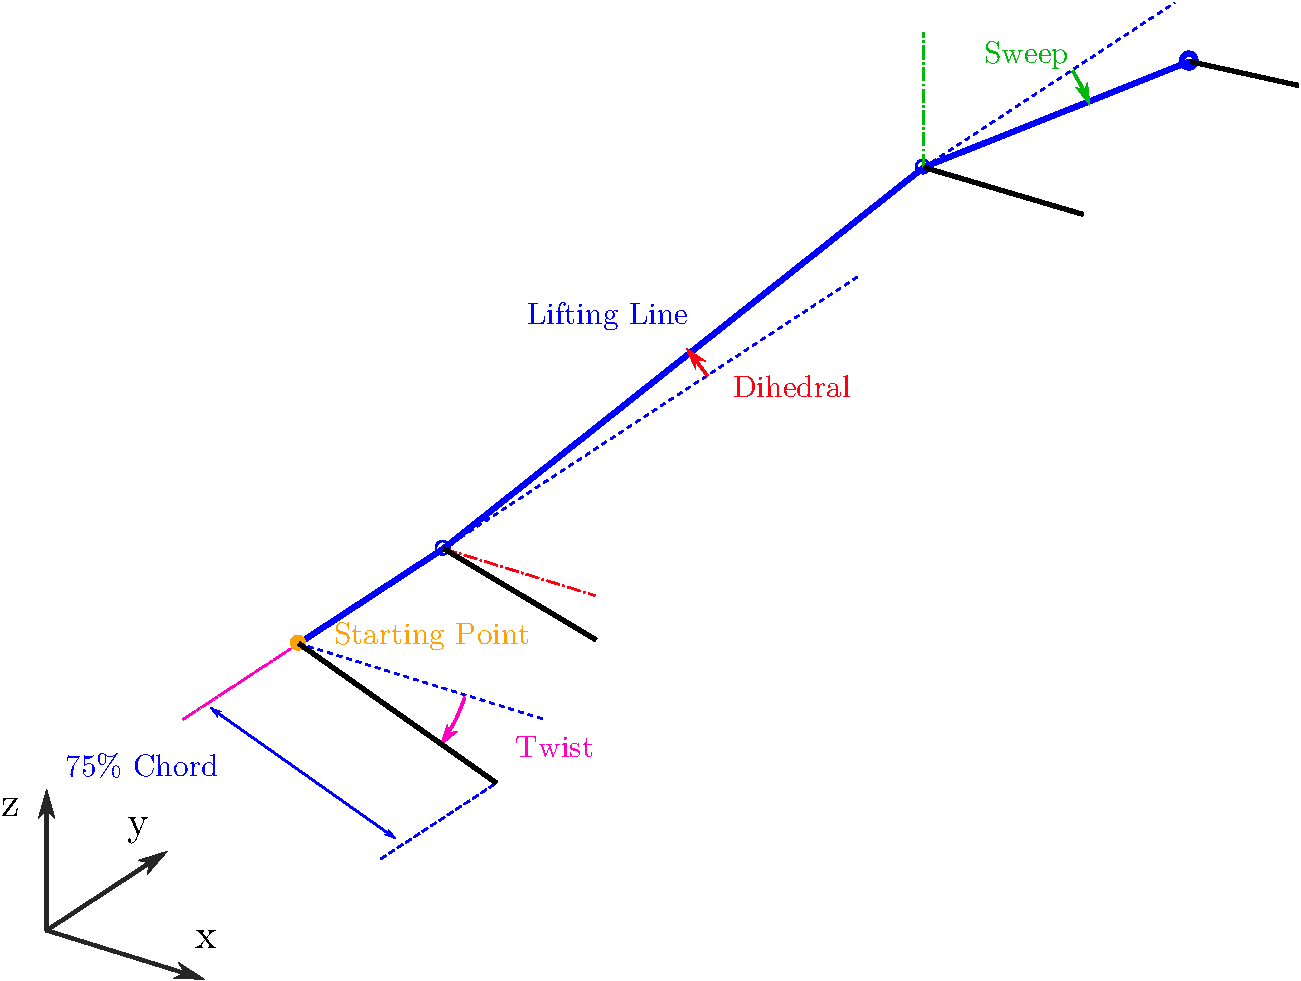
\includegraphics[width=.7\textwidth]{parametric_sections_ll}
\caption{Generation logic of the geometry of parametric lifting lines.}
\label{fig:parametric_sections_ll}
\end{figure}

Finally it is important to stress that the reference frames introduced in the present section 
concerning the generation of parametric components are local to those component, and are required 
only to assign coordinates to the points generated parametrically, just as a mesh generated from 
CAD files and an external mesher will generate points in a certain reference frame. 
The actual position of the component in space during the simulation depends on the reference 
frame in which the component will be introduced. Reference frames employed during the simulation 
are discussed in section \ref{sec:Solver_ReferenceFrames}.

\subsection{Hinged Surfaces}
\label{sec:Hinge_surfaces}
It is possible to introduce one or more movable surfaces in the parametric definition of a wing.
As outlined by the scheme in Fig. \ref{fig:hinge} left, in a two-dimensional problem the control 
surface can be defined in the local reference frame of the component, by means of the hinge axis 
position $H$, the chordwise direction $\xi$ and a blending region $[-u, u]$ 
(defined by \param{hinge\_Offset} parameter)introduced to avoid irregular behavior of the 
mesh along with the rotation angle $\theta$.
\begin{figure}[htbp]
\vspace{-3cm}
\centering
    \def\svgwidth{\columnwidth}
    %% Creator: Inkscape inkscape 0.92.4, www.inkscape.org
%% PDF/EPS/PS + LaTeX output extension by Johan Engelen, 2010
%% Accompanies image file 'hinges.eps' (pdf, eps, ps)
%%
%% To include the image in your LaTeX document, write
%%   \input{<file_name>.pdf_tex}
%%  instead of
%%   \includegraphics{<file_name>.pdf}
%% To scale the image, write
%%   \def\svgwidth{<desired width>}
%%   \input{<file_name>.pdf_tex}
%%  instead of
%%   \includegraphics[width=<desired width>]{<file_name>.pdf}
%%
%% Images with a different path to the parent latex file can
%% be accessed with the `import' package (which may need to be
%% installed) using
%%   \usepackage{import}
%% in the preamble, and then including the image with
%%   \import{<path to file>}{<file_name>.pdf_tex}
%% Alternatively, one can specify
%%   \graphicspath{{<path to file>/}}
%% 
%% For more information, please see info/svg-inkscape on CTAN:
%%   http://tug.ctan.org/tex-archive/info/svg-inkscape
%%
\begingroup%
  \makeatletter%
  \providecommand\color[2][]{%
    \errmessage{(Inkscape) Color is used for the text in Inkscape, but the package 'color.sty' is not loaded}%
    \renewcommand\color[2][]{}%
  }%
  \providecommand\transparent[1]{%
    \errmessage{(Inkscape) Transparency is used (non-zero) for the text in Inkscape, but the package 'transparent.sty' is not loaded}%
    \renewcommand\transparent[1]{}%
  }%
  \providecommand\rotatebox[2]{#2}%
  \newcommand*\fsize{\dimexpr\f@size pt\relax}%
  \newcommand*\lineheight[1]{\fontsize{\fsize}{#1\fsize}\selectfont}%
  \ifx\svgwidth\undefined%
    \setlength{\unitlength}{489.93968126bp}%
    \ifx\svgscale\undefined%
      \relax%
    \else%
      \setlength{\unitlength}{\unitlength * \real{\svgscale}}%
    \fi%
  \else%
    \setlength{\unitlength}{\svgwidth}%
  \fi%
  \global\let\svgwidth\undefined%
  \global\let\svgscale\undefined%
  \makeatother%
  \begin{picture}(1,0.43599908)%
    \lineheight{1}%
    \setlength\tabcolsep{0pt}%
    \put(0,0){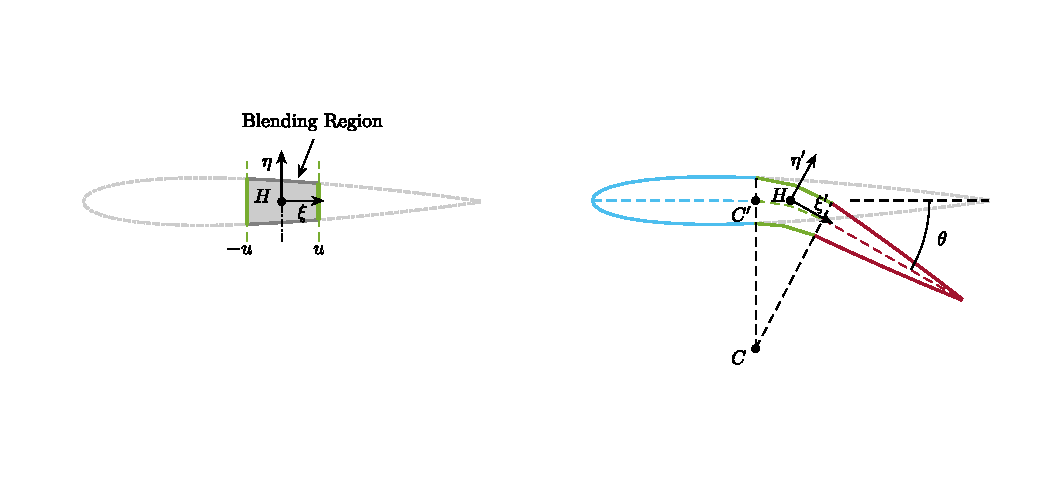
\includegraphics[trim={0 1.5cm 0 1.5cm},clip, width=\unitlength]{./images/hinges.eps}}%
  \end{picture}%
\endgroup%

    \caption{Scheme of the two-dimensional hinged surface configuration}
    \label{fig:hinge}
\end{figure}
Three regions are defined using the coordinates defined through this reference frame:
\begin{enumerate}
  \item $\xi \leq -u$: no influence of the aileron rotation;
  \item $\xi \geq  u$: rigid rotation around the hinge;
  \item $-u \le \xi \le  u$: blending region for avoiding irregular behavior defined as an 
  arc of a circle whose center is locate on point $C$;
\end{enumerate}
In a three-dimensional problem, the reference configuration of a control surface, 
as an aileron, is defined in wind axis reference frame of the component.
\begin{figure}[htbp]
    \centering
    \def\svgwidth{\columnwidth}
    %% Creator: Inkscape inkscape 0.92.4, www.inkscape.org
%% PDF/EPS/PS + LaTeX output extension by Johan Engelen, 2010
%% Accompanies image file 'hinge_ref_system.pdf' (pdf, eps, ps)
%%
%% To include the image in your LaTeX document, write
%%   \input{<filename>.pdf_tex}
%%  instead of
%%   \includegraphics{<filename>.pdf}
%% To scale the image, write
%%   \def\svgwidth{<desired width>}
%%   \input{<filename>.pdf_tex}
%%  instead of
%%   \includegraphics[width=<desired width>]{<filename>.pdf}
%%
%% Images with a different path to the parent latex file can
%% be accessed with the `import' package (which may need to be
%% installed) using
%%   \usepackage{import}
%% in the preamble, and then including the image with
%%   \import{<path to file>}{<filename>.pdf_tex}
%% Alternatively, one can specify
%%   \graphicspath{{<path to file>/}}
%% 
%% For more information, please see info/svg-inkscape on CTAN:
%%   http://tug.ctan.org/tex-archive/info/svg-inkscape
%%
\begingroup%
  \makeatletter%
  \providecommand\color[2][]{%
    \errmessage{(Inkscape) Color is used for the text in Inkscape, but the package 'color.sty' is not loaded}%
    \renewcommand\color[2][]{}%
  }%
  \providecommand\transparent[1]{%
    \errmessage{(Inkscape) Transparency is used (non-zero) for the text in Inkscape, but the package 'transparent.sty' is not loaded}%
    \renewcommand\transparent[1]{}%
  }%
  \providecommand\rotatebox[2]{#2}%
  \newcommand*\fsize{\dimexpr\f@size pt\relax}%
  \newcommand*\lineheight[1]{\fontsize{\fsize}{#1\fsize}\selectfont}%
  \ifx\svgwidth\undefined%
    \setlength{\unitlength}{1473.59524082bp}%
    \ifx\svgscale\undefined%
      \relax%
    \else%
      \setlength{\unitlength}{\unitlength * \real{\svgscale}}%
    \fi%
  \else%
    \setlength{\unitlength}{\svgwidth}%
  \fi%
  \global\let\svgwidth\undefined%
  \global\let\svgscale\undefined%
  \makeatother%
  \begin{picture}(1,0.50285178)%
    \lineheight{1}%
    \setlength\tabcolsep{0pt}%
    \put(0,0){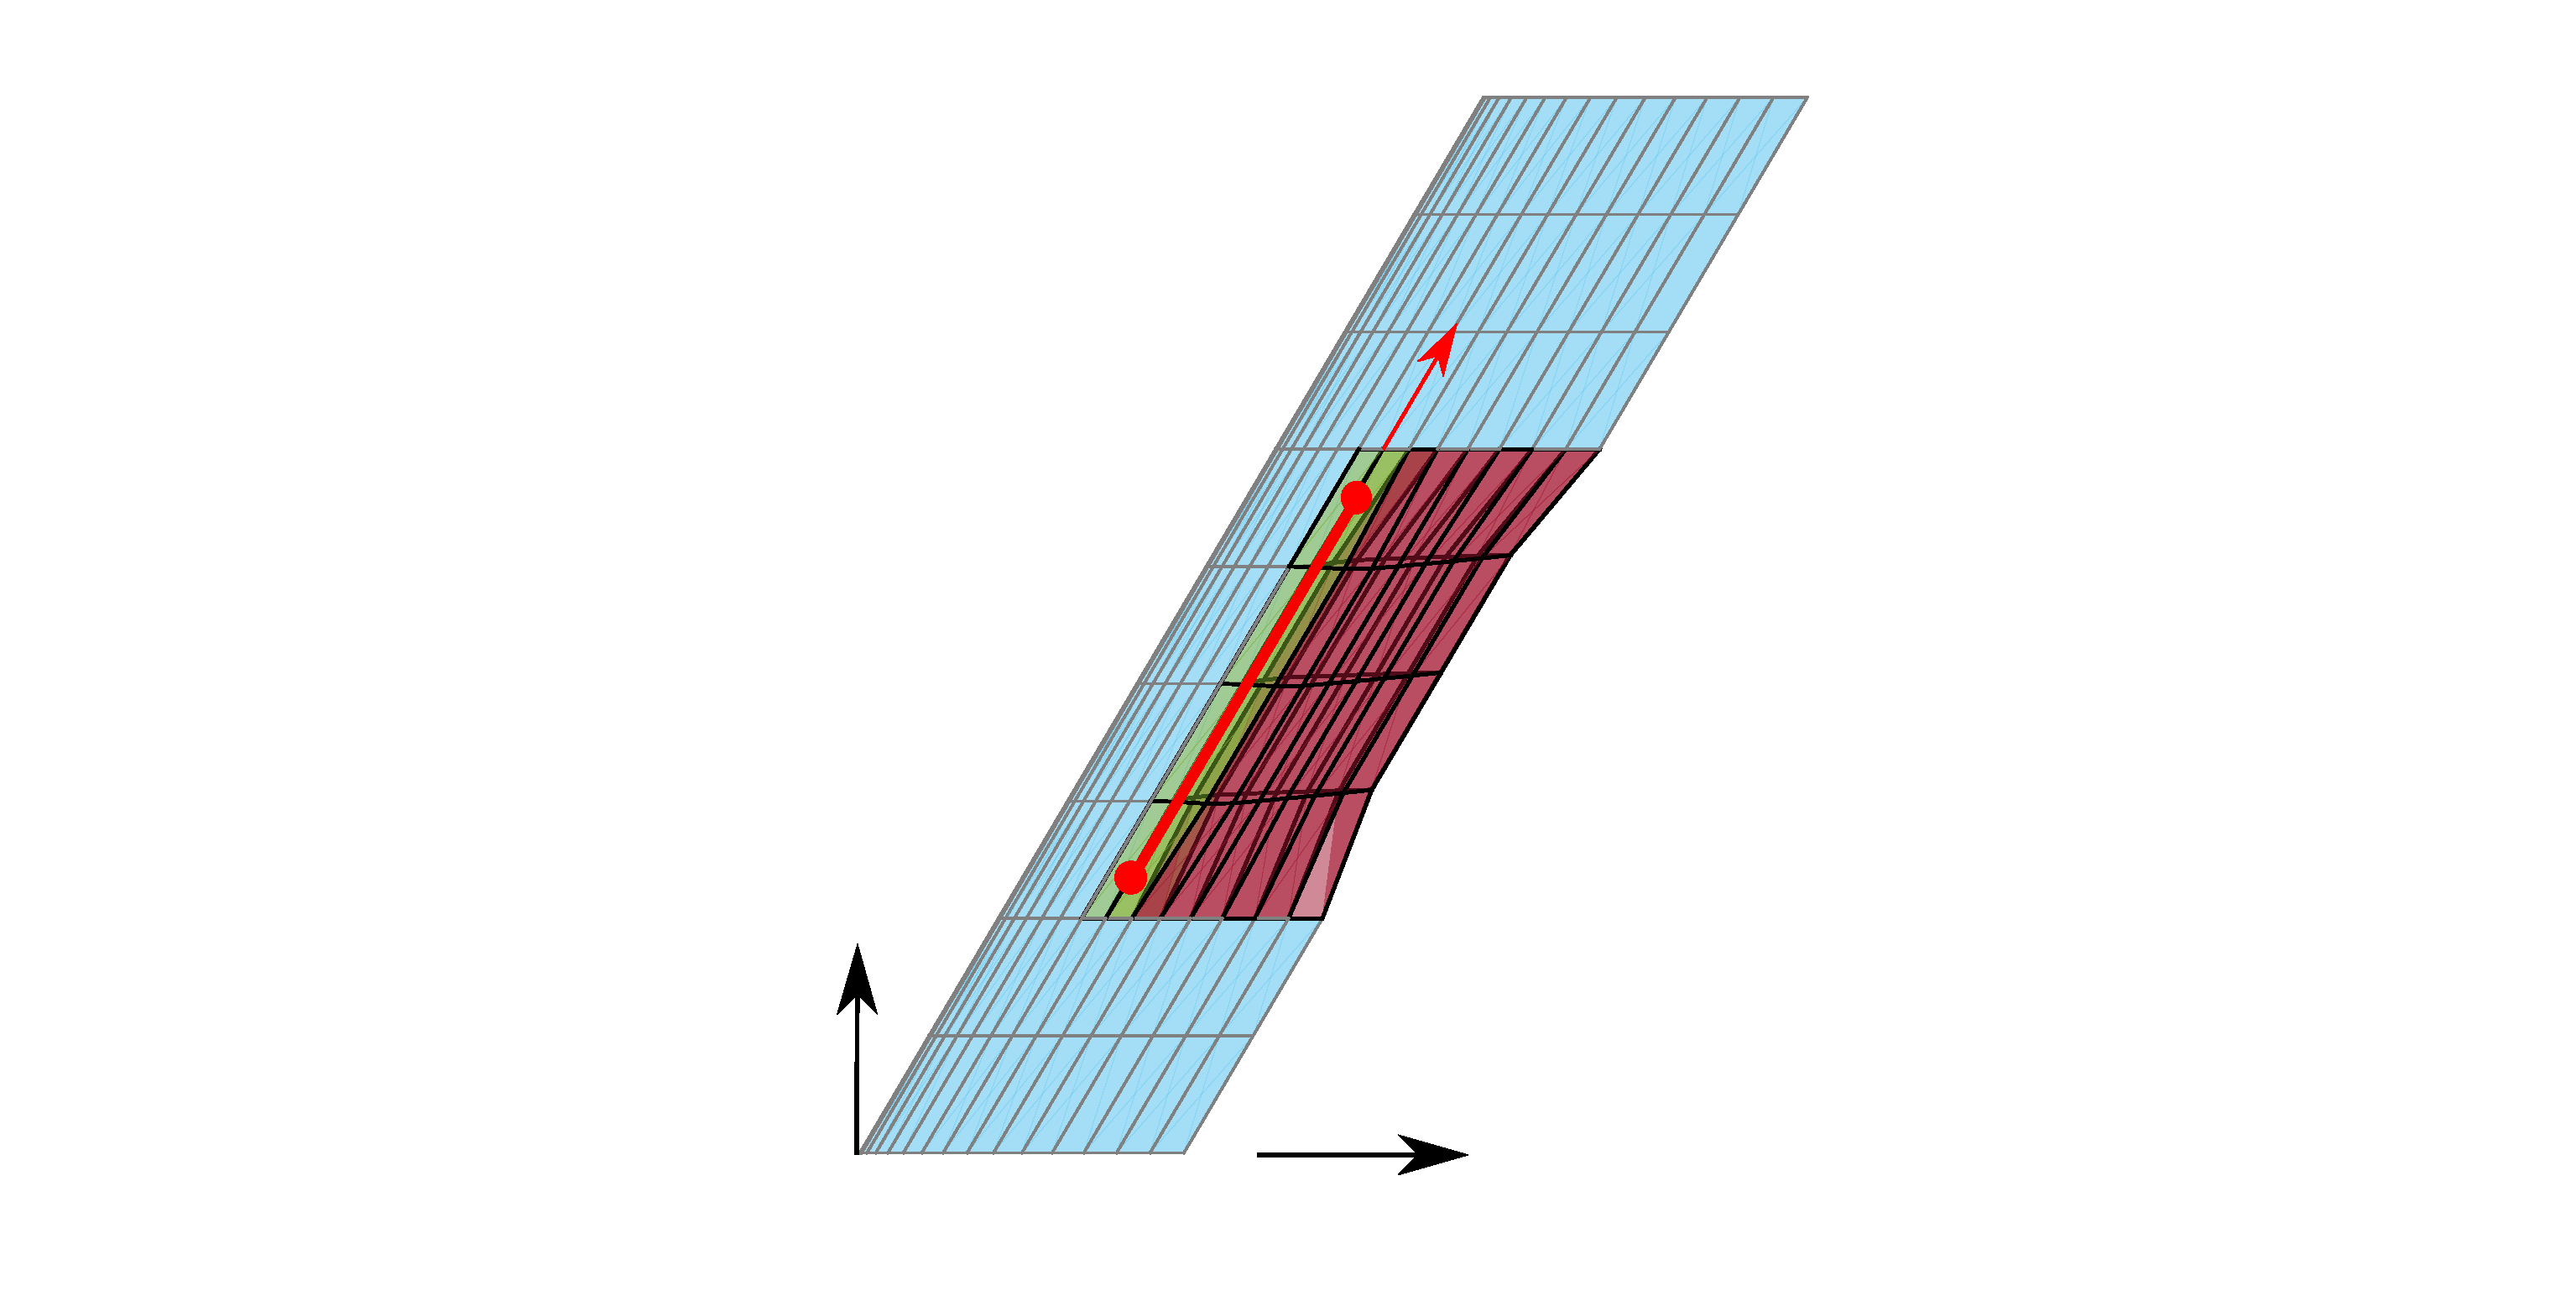
\includegraphics[width=\unitlength,page=1]{./images/hinge_ref_system.pdf}}%
    \put(0.52884911,0.07256303){\color[rgb]{0,0,0}\makebox(0,0)[lt]{\lineheight{1.25}\smash{\begin{tabular}[t]{l}$x_{dust}$\end{tabular}}}}%
    \put(0.27727265,0.12854856){\color[rgb]{0,0,0}\makebox(0,0)[lt]{\lineheight{1.25}\smash{\begin{tabular}[t]{l}$y_{dust}$\end{tabular}}}}%
    \put(0.5592075,0.33231148){\color[rgb]{0,0,0}\makebox(0,0)[lt]{\lineheight{1.25}\smash{\begin{tabular}[t]{l}$\Vec{h}$\end{tabular}}}}%
    \put(0.40960207,0.17181009){\color[rgb]{0,0,0}\makebox(0,0)[lt]{\lineheight{1.25}\smash{\begin{tabular}[t]{l}A\end{tabular}}}}%
    \put(0.50467099,0.31395518){\color[rgb]{0,0,0}\makebox(0,0)[lt]{\lineheight{1.25}\smash{\begin{tabular}[t]{l}B\end{tabular}}}}%
  \end{picture}%
\endgroup%

    \caption{hinge reference system for a swept wing}
    \label{fig:hingeref}
\end{figure}

The aerodynamic sections that are involved in the control surface are then the 
ones that satisfy the condition $y(A) < y(P) < y(B)$, where $y(P)$ is the 
ordinate of the $P_i-th$ aerodynamic mesh point expressed in the wind reference system. 
As in the 2D case, we can then define the three regions for each stripe identified 
at the previous point. The y coordinate of the origin of the sectional reference 
frame is determined by linear interpolation between points A and B. 
Points A and B corresponds to the user input \param{node_1} and \param{node_2}, respectively. 
The rotation axis is defined by $\Vec{h} = (B - A)$.

% input file
\begin{inputfile}[frame=single, caption={Parametric geometry for flapped wing}, 
  label={file:parametric_example_flapped_wing.in}]
mesh_file_type = parametric
el_type = p
scale_factor = 1.0
offset = (/0.0 , 0.0,  0.0/)

mesh_symmetry = T
symmetry_point   = (/0.0 , 0.0,  0.0/)
symmetry_normal = (/0.0 , 1.0,  0.0/)

nelem_chord = 15
type_chord = cosineLE   ! uniform  cosineLE  cosineTE
starting_point = (/0.0,0.0,0.0/)
reference_chord_fraction = 0.25

n_hinges = 2
hinge = {
  hinge_tag = aileron_right
  hinge_nodes_input = parametric      ! or from_file
  node_1 = (/ 1.4178, 1.4557, 0.3473/)  ! In the local ref.frame
  node_2 = (/ 2.4026  , 3.1615  , 0.6946/)
  n_nodes = 2
  ! }
  ! hinge_nodes_input_from_file = {
  !   node_file = hinge_node.dat
  ! }
  hinge_ref_dir = (/ 1.0, 0.0 , 0.0 /)
  hinge_offset  = 0.1
  hinge_spanwise_blending = 0.01
  hinge_rotation_input = function:sin
  hinge_rotation_function = {
    amplitude = 30.0    ! deg
    omega     =  12.5   ! rad/sec
    phase     =  0.0    ! deg
  }

hinge = {
  hinge_tag = aileron_left
  hinge_nodes_input = parametric      
  node_2 = (/ 1.4178, -1.4557, 0.3473/)  
  node_1 = (/ 2.4026  , -3.1615  , 0.6946/)
  n_nodes = 2
  ! }
  ! hinge_nodes_input_from_file = {
  !   node_file = hinge_node.dat
  ! }
  hinge_ref_dir = (/ 1.0, 0.0 , 0.0 /)
  hinge_offset  = 0.1
  hinge_merge_tol = 0.01
  hinge_spanwise_blending = 0.01
  hinge_rotation_input = function:sin
  hinge_rotation_function = {
    amplitude = -30.0    ! deg
    omega     =  12.5    ! rad/sec
    phase     =  0.0     ! deg
  }


! First section
chord = 2
twist = 0.0
airfoil = NACA0012

! First region
span = 5.0
sweep = 30.0
dihed = 10.0
nelem_span = 20
type_span = uniform

! Second section
chord = 2
twist = 0.0
airfoil = NACA0012
\end{inputfile}

All the detailed parameters of the Hinged surfaces input file are: 
\begin{itemize}
    \item \param{n\_hinge}: \textit{required:} no.  \textit{multiple:} no. \textit{default:} 0.
    \textit{type:} integer
    
    Number of hinges and rotating parts (e. g. aileron) of the component.
    
    \item \param{hinge\_Tag}: \textit{required:} no. \textit{multiple:} same number as \param{n\_hinge} \textit{type:} string 
    
    name of the control surface.
    
    \item \param{hinge\_Nodes\_Input}: \textit{required:} yes. \textit{multiple:} no. \textit{type:} string
    
    type of hinge nodes input: \opt{parametric} or \opt{from\_file}. (TODO add details)
    
    \item \param{node_1} \textit{required:} yes. \textit{multiple:} no. \textit{type:} real array, length 3.
    
    First node of the hinge. Components in the local reference frame of the component.
    
    \item \param{node_2} \textit{required:} yes. \textit{multiple:} no. \textit{type:} real array, length 3.
    
    Second node of the hinge. Components in the local reference frame of the component.
    
    \item \param{hinge\_ref\_dir} \textit{required:} yes. \textit{multiple:} no. \textit{type:} real array, length 3. 
    
    Reference direction of the hinges, indicating zero-deflection direction in the local reference frame of the component.
    
    \item \param{hinge\_merge\_tol} \textit{required:} no. \textit{multiple:} no. \textit{type:} real. \textit{default:} 0.01
    
    Tolerance for adaptive hinge mesh in chord adimensional length. 
    
    \item \param{hinge\_offset} \textit{required:} no. \textit{multiple:} no. \textit{type:} real. \textit{default:} 0.
    
    offset in the \param{hinge\_ref\_dir} needed for avoiding irregular behavior of the surface for large deflections.

    \item \param{hinge\_spanwise\_blending} \textit{required:} no. \textit{multiple:} no. \textit{type:} real. \textit{default:} 0.
    
    Blending in the spanwise direction needed for avoiding irregular behavior of the surface for large deflections.
    
    \item \param{hinge\_rotation\_input}
    \textit{required:} yes. \textit{type:} string.
    
    input type of the rotation: \opt{function}, \opt{from\_file} or \opt{coupling}. 
    If the chosen option is \opt{coupling}, then the component must be coupled with preCICE (\param{coupling} \opt{T}).
    
    \item \param{hinge\_rotation\_function}: \textit{required:} no. \textit{type:} string. 
    
    Parser for hinge input with simple functions; the supported functions are: 
    \opt{function:const}, \opt{function:sin}, \opt{function:cos}. 
    \begin{itemize}
        \item \param{amplitude} \textit{required:} yes. \textit{type:} real. 
        
        amplitude of the rotation in degrees for constant, cosine and sine functions. 
        
        \item \param{omega} \textit{required:} yes. \textit{type:} real. \textit{default:} 0.0 
        
        Angular velocity of the rotation function in \si{\deg\per\second}, for constant?, cosine and sine functions.
        
        \item \param{phase} \textit{required:} yes. \textit{type:} real. \textit{default:} 0.0
        
        phase angle of the rotation function in \si{\deg}, for constant?, cosine and sine functions.
    \end{itemize}
    \item \param{hinge\_Rotation\_File} \textit{required:} no. \textit{type:} string. 
    
    Parser for hinge input from file
    
    \begin{itemize}
        \item \param{file_name} \textit{required:} yes. \textit{type:} string. 
        
        name of the file containing the input of the hinge rotation
    \end{itemize}
    
    \item \param{hinge\_rotation\_coupling} \textit{required:} no. \textit{type:} string.
    
    Parser for hinge input from coupling (see~\ref{subsec:DUSTpreCICE})
    
    \begin{itemize}
        \item \param{coupling\_node\_subset} \textit{required:} no. \textit{type:} string.
        
        Define a subset of structural nodes to evaluate coupling: \opt{range} or \opt{from\_file}
        
        \item \param{coupling\_node\_first} \textit{required:} no. \textit{type:} integer. 
        
        If node subset is defined through \opt{range} input: first ID of the nodes
        
        \item \param{coupling\_node\_last} \textit{required:} no. \textit{type:} integer. 
        
        If node subset is defined through \opt{range} input: last ID of the nodes
        
        \item \param{coupling\_node\_filename} \textit{required:} no. \textit{type:} string.
        
        file collecting the IDs of the coupling nodes for hinge coupling
    \end{itemize}
    
    

    
\end{itemize}




\section{Pointwise mesh generation}
\label{sec:Pointwise_mesh_generation}
%
The \param{pointwise} mesh definition extends the capabilities of the \param{parametric} input. 
First, the reference line of the component is defined as a list of points connected with straight 
lines or Hermitian splines. The sections of a component are defined at each input points by means 
of their plane coordinates, their dimensions and rotation around an axis perpendicular to their own plane.
%
The input file is mainly composed of three sections: a generic section for the types of the 
aerodynamic elements and the symmetry and mirroring options, a section for the \param{point} 
list and a section for the \param{Line}. The parameters of the first section are very similar 
to the ones used in the \param{parametric} description, except for the \param{starting\_point}, 
that is not needed here, since the point with \param{Id}$=1$ is meant to be the first point of 
the reference line.
\newline \noindent
%
An example of input file for \param{pointwise}-defined component is provided in file 
\ref{file:pointwise_example_file.in}. The description of this file and all the parameters follows.
%

\begin{inputfile}[frame=single, caption={''Pointwise'' geometry definition }, label={file:pointwise_example_file.in}]
mesh_file_type = pointwise
el_type = p

mesh_symmetry = T
symmetry_point = (/0.0,0.0,0.0/)
symmetry_normal = (/0.0,1.0,0.0/)

mesh_mirror = F
mirror_point = (/0.0,0.0,0.0/)
mirror_normal = (/0.0,1.0,0.0/)

reference_chord_fraction = 0.0

mesh_flat = F

nelem_chord = 20
type_chord = cosineLE

! === Points ===
point = {
  id = 1
  coordinates = (/ 0.0 , 0.0 , 0.0 /)
  airfoil = NACA2412
  chord = 1.0
  twist = 5.0
  section_normal = yAxis
}
point = {
  id = 2
  coordinates = (/ 1.5 , 3.0 , 0.3 /)
  airfoil = NACA2412
  chord = 0.4
  twist = 0.0
  section_normal = yAxis
}
point = {
  id = 3
  coordinates = (/ 1.8 , 3.5 , 0.7 /)
  airfoil = NACA2412
  chord = 0.3
  twist = 0.0
  section_normal = reference_line ! (default)
}
point = {
  Id = 4
  Coordinates = (/ 2.1 , 3.5 , 1.1 /)
  airfoil = NACA2412
  chord = 0.3
  twist = 0.0
  section_normal = reference_line ! (default)
}
point = {
  id = 5
  coordinates = (/ 2.4 , 3.0 , 1.4 /)
  airfoil = NACA2412
  chord = 0.4
  twist = 0.0
  section_normal = y_axis_neg
  flip_section = T
}
point = {
  id = 6
  coordinates = (/ 3.5 , 0.0 , 1.5 /)
  airfoil = NACA2412
  chord = 1.0
  twist = 5.0
  section_normal = y_axis_neg
  flip_section = T
}

! === Lines ===
line = {
  type = straight
  end_points = (/ 1 , 2 /)
  nelems = 5
}
line = {
  type = spline
  end_points = (/ 2 , 5 /)
  nelems = 10
  ! see documentation for optional inputs
}
line = {
  type = straight
  end_points = (/ 5 , 6 /)
  nelems = 5
}

\end{inputfile}
%
\begin{figure}[h!]
\centering
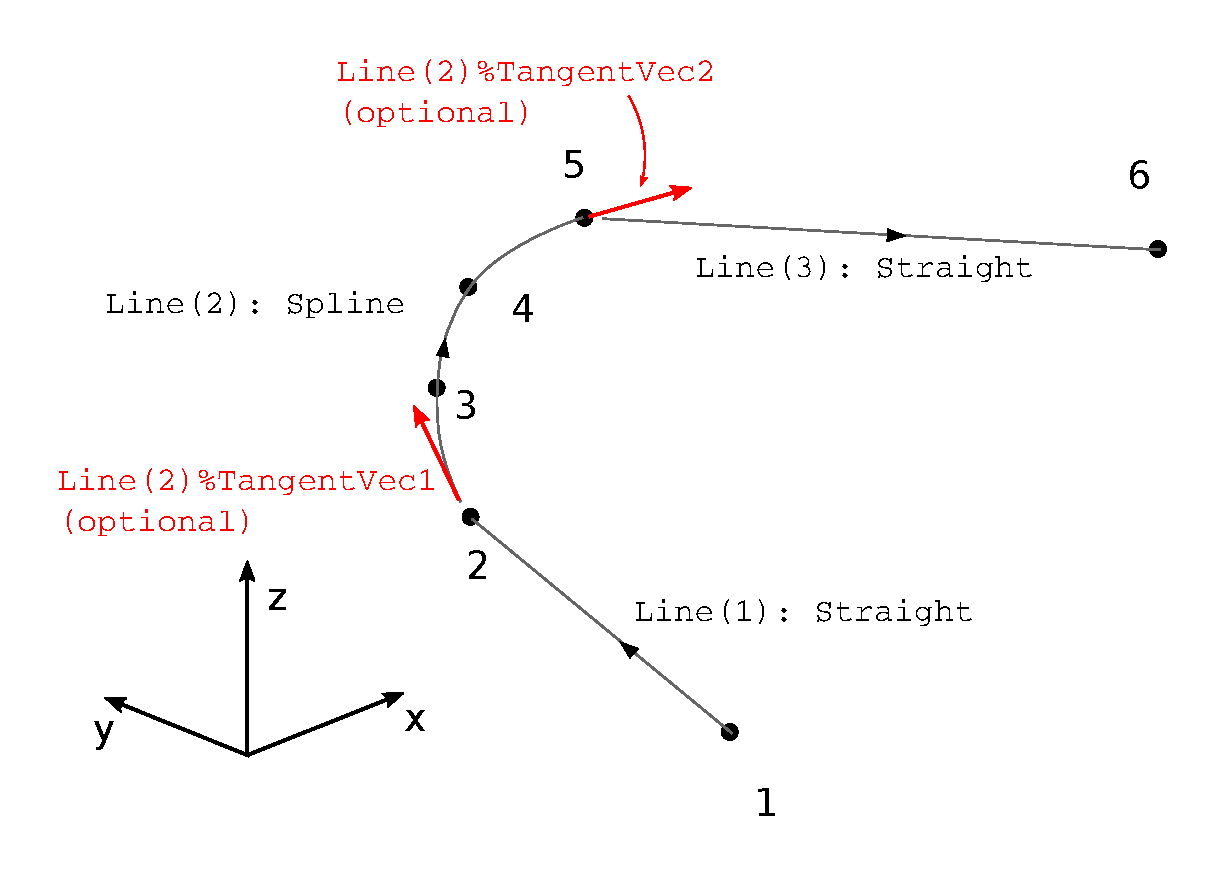
\includegraphics[width=.50\textwidth]{pointwise_2_referenceLine}
    \caption{Pointwise definition of a component: reference line by 
    \param{point}s and \param{Line}s connecting them.}
\label{fig:pointwise_reference_line}
\end{figure}
%
\begin{figure}[h!]
\centering
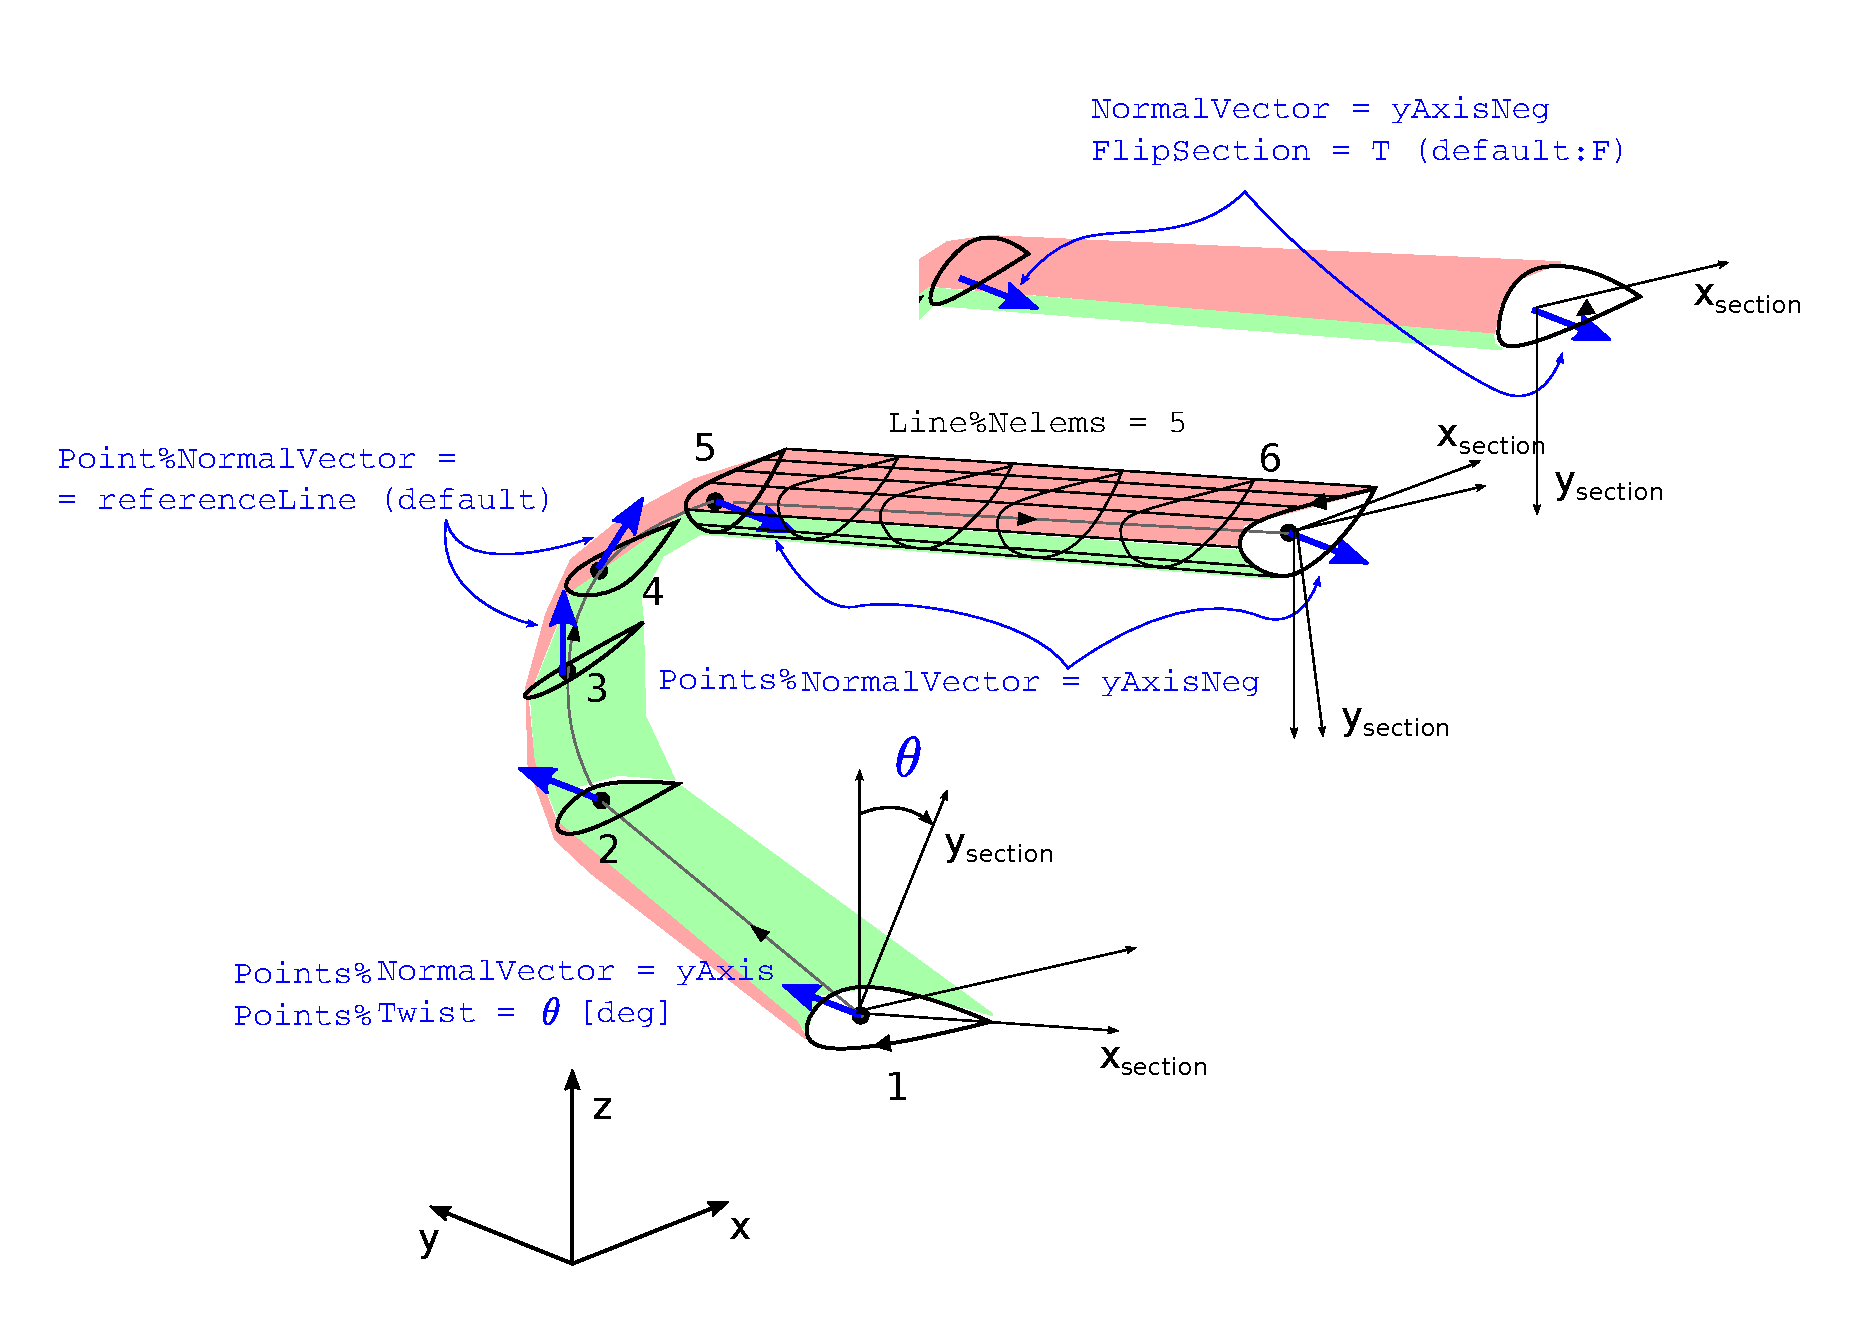
\includegraphics[width=.70\textwidth]{pointwise_3_component_flip}
    \caption{Pointwise definition of a component: section parameters 
    (\param{airfoil}, \param{chord}, \param{twist}, \param{section_normal}) at 
    \param{point}s of the reference line and the number \param{nelems} of 
    elements along the reference line for each \param{line}. 
    The parameter \param{flip\_section} can be set to \param{.true.} 
    in order to flip the $y$-coordinate of the airfoil, in the section 
    reference frame: the comparison between the goemetry with 
    \param{flip\_section} equal to \param{F} or \param{T}  at \param{point} with 
    \param{id} = 5, 6 is shown in the picture for a non-symmetrical airfoil.}
\label{fig:pointwise_component}
\end{figure}


\begin{itemize}

\item \param{mesh_file_type}: \textit{required:} yes. \textit{multiple:} no. \textit{type:} string. 

Use \param{pointwise} for pointwise geometry.

\item \param{el_type}: \textit{required:} yes. \textit{multiple:} no. \textit{type:} character.

    type of the elements of the mesh. \opt{p} stands for surface panels to model 
    solid bodies, \opt{v} stands for vortex lattice elements used to model flat surfaces, 
    {\color{red}\opt{l} stands for lifting lines used to produce a 1D model of a lifting surface}. 

\item \param{mesh\_symmetry} \textit{required:} no. \textit{multiple:} no. \textit{default:} false. \textit{type:} logical.

Choose to reflect the mesh around a point and a direction. Useful to produce full meshes out of 
symmetrical half models. Keeps both the original and the symmetrical part. 

\item \param{symmetry\_point}: \textit{required:} only if \param{mesh\_reflection} is true. 
\textit{multiple:} no. \textit{default:} (0.0, 0.0, 0.0). \textit{type:} real array, length 3.

point around which to reflect the mesh.

\item \param{symmetry\_normal}: \textit{required:} only if \param{mesh\_reflection} is true. 
\textit{multiple:} no. \textit{default:} (0.0, 1.0, 0.0). \textit{type:} real array, length 3.

Direction in which to reflect the mesh.

\item \param{mesh\_mirror} \textit{required:} no. \textit{multiple:} no. \textit{default:} 
false. 
\textit{type:} logical.

Choose to mirror the mesh around a point and a direction. Same as \param{mesh\_symmetry}, but 
does not keep both the original, i.e. the mesh is not doubled.

\item \param{mirror\_point}: \textit{required:} only if \param{mesh\_reflection} is true. 
\textit{multiple:} no. \textit{default:} (0.0, 0.0, 0.0). \textit{type:} real array, length 3.

point around which to mirror the mesh.

\item \param{mirror\_normal}: \textit{required:} only if \param{mesh\_reflection} is true. 
\textit{multiple:} no. \textit{default:} (0.0, 1.0, 0.0). \textit{type:} real array, length 3.

Direction in which to mirror the mesh.

\item \param{reference\_chod\_fraction} \textit{required:} no. \textit{multiple:} no. 
\textit{default:} 0.0 \textit{type:} real

Fraction of the chord at which to place the axis which will be rotated of the sweep 
and dihedral angles, and around which airfoils are twisted. 

\item \param{mesh\_flat} \textit{required:} no. \textit{multiple:} no. 
\textit{default:} true \textit{type:} logical

Used only in case of lifting lines (\opt{l}) elements. If enabled instead of 
generating lifting lies actually twisted according to the input twist, 
but rather a flat surface with only the normal vectors twisted according 
to the input twist. 

\item \param{nelem\_chord} \textit{required:} yes, if parametric. 
\textit{multiple:} no. \textit{type:} integer.

Number of elements in chord direction. Note: if the elements are vortex 
lattice $nelem\_chord$ elements will be generated, while in case of 
surface panels $2nelem\_chord$ elements will be produced, $nelem\_chord$ 
on the lower and $nelem\_chord$ on the upper side. In case of lifting lines 
this parameter is ignored.

\item \param{type\_chord} \textit{required:} no. \textit{multiple:} no. 
\textit{default:} \param{uniform} \textit{type:} string.

type of subdivision in the chord-wise direction. Can be \opt{uniform} 
for a uniform distribution, \opt{cosine} for a cosine distribution, 
refined both on the leading and trailing edge, \opt{cosineLE} for a 
half cosine refined only on leading edge or \opt{cosineTE} for a half 
cosine refined only on the trailing edge. 

\end{itemize}
%
A list of \param{point} groups follows. These points are used to 
describe the reference line of the component. The parameters of a 
\param{point} element are:
\begin{itemize}

\item \param{id} \textit{required}: yes, \textit{multiple}: no, \textit{type}: integer.

    Id. number of the \param{point}, used in the point-to-line 
    connectivity defined in \param{line} groups.

\item \param{coordinates}  \textit{required}: yes, \textit{multiple}: 
      no, \textit{type:} real array, length 3.

    Coordinates of the point in the local reference frame of the component.
    
\item \param{airfoil}  \textit{required}: yes, \textit{multiple}: no, \textit{type}: string.

    Same as in the parametric definition of a component. To be used for vortex 
    lattices or surface panels
    
\item \param{airfoil\_table}  \textit{required}: yes, \textit{multiple}: no, 
    \textit{type}: string.

    Same as in the parametric definition of a component. 
    To be used for lifting lines only in place of \param{airfoil}

\item \param{chord}  \textit{required}: yes, \textit{multiple}: no, \textit{type}: real.

    Define section dimensions, by its chord length.

\item \param{twist}  \textit{required}: yes, \textit{multiple}: no, \textit{type}: real.

    Angle of twist, in degrees, of the airfoil section. rotation around 
    the vector that is normal to the plane of the section.

\item \param{section\_normal} \textit{required}: no, \textit{multiple}: no , 
\textit{default}: \param{reference_line} , \textit{type}: string.

    String to define the plane of the section. It can be: \param{reference_line}, 
    for sections perpendicular to the reference line; \param{y_axis}, 
    \param{y_axis_neg} for sections perpendicular to the $y$-axis or 
    $-y$-axis of the component local reference frame; \param{vector}, 
    to define a generic vector. 

\item \param{section\_normal\_vector} \textit{required}: only if 
\param{section\_normal = vector}, \textit{multiple}: no, \textit{type}: real array, length 3.

    Components of the normal vector of the section, if \param{section\_normal = vector}.

\item \param{flip\_section} \textit{required}: no, \textit{multiple}: no, 
\textit{default}: \param{F} , \textit{type}: logical.

  Flip the $y$ coordinates in the section reference frame. 
  Meant to help the pointwise definition of close wing configurations.

\end{itemize}
%
A list of \param{line} groups follows. These lines are used to build the 
reference line of the component connecting the points defined above. 
The parameters of a \param{line} element are:
\begin{itemize}

\item \param{type} \textit{required}: yes, \textit{multiple}: no, \textit{type}: string.

    Line type. It can be: \param{straight} for straight lines, 
    \param{spline} for Hermitian splines.

\item \param{end_points}  \textit{required}: yes, \textit{multiple}: no, 
\textit{type}: integer array, lenght 2.

    \param{id} numbers of the beginning and ending \param{point}s of the line. 
    For \param{straight} lines, this two numbers must be consecutive. 
    For \param{spline}s the spline is built using these ones as the first 
    and last points and all the points with \param{Id} in between as interior 
    points, so that they must exist in the point list.

\item \param{nelems}  \textit{required}: yes, \textit{multiple}: no, \textit{type}: integer.

    Number of elements in the direction of the reference line belonging 
    to this region.

\item \param{type\_span} \textit{required}: no, \textit{multiple}: no, 
\textit{default}: \param{uniform}, \textit{type}: string.

    type of refinement of the elements in the spanwise direction. 
    As for the chordwise direction, the options are \opt{uniform} 
    for a uniform distribution, \opt{cosine} for a cosine refinement 
    both inboard and outboard, and \opt{cosineIB} and \opt{cosineOB} 
    for half cosine refinement only inboard or outboard. 
  
\item \param{tangent\_vec1} \textit{required}: if \param{Line\%type = spline} 
and \param{Line\%end\_points(1) = 1}, \textit{multiple}: no, 
\textit{type}: real array, length 3. 

    Tangent vector at the first point of a \param{spline}. 
    This is an optional input for \param{spline}. If this field 
    is not present, the spline inherits the tangent vector from the 
    neighboring line (that must be a \param{straight} line).

\item \param{tangent\_vec2} \textit{required}: if \param{Line\%type = spline} 
and \param{Line\%EndPoints(2)} is the last point of the reference line, 
\textit{multiple}: no, \textit{type}: real array, length 3. 

    Tangent vector at the last point of a \param{spline}. 
    This is an optional input for \param{spline}. If this field is 
    not present, the spline inherits the tangent vector from the 
    neighboring line (that must be a \param{straight} line).

\item \param{tension} \textit{required}: no, \textit{multiple}: no, 
\textit{default}: 0.0 , \textit{type}: real.

    \param{tension} parameter of the Hermitian \param{spline}.

\item \param{bias} \textit{required}: no, \textit{multiple}: no, 
\textit{default}: 0.0 , \textit{type}: real.

    \param{bias} parameter of the Hermitian \param{spline}.

\end{itemize}

\subsection{Hermitian splines}
The Hermitian splines by the following expression,
\begin{equation}
\mathbf{r}_i(t) = \mathbf{r}_{i-1} h_0(t) + \mathbf{r}_{i} h_1(t) +
                  \mathbf{d}_{i-1} h_2(t) + \mathbf{d}_{i} h_3(t) \ ,
\end{equation}
where $h_i(t), \ i=0:3$ are the Hermitian functions, 
the points $\mathbf{r}_i$ are the points to be interpolated, 
$\mathbf{d}_i$ the approximation of the derivatives at the interpolation 
points. For the interior points of a spline,
\begin{equation}
\begin{aligned}
\mathbf{d}_i & = 0.5 ( \mathbf{r}_{i+1} - \mathbf{r}_{i  } ) \ 
                      (1-\param{bias}) (1-\param{tension}) \\
             & + 0.5 ( \mathbf{r}_{i  } - \mathbf{r}_{i-1} ) \ 
                    (1+\param{bias}) (1-\param{tension}) \ .
\end{aligned}
\end{equation}
The \param{bias} parameter is a weight on the finite difference 
computed using forward and backward differences, while \param{tension} 
acts like a tensile action on the spline, see figure \ref{fig:spline_tension}.
\begin{figure}[h!]
\centering
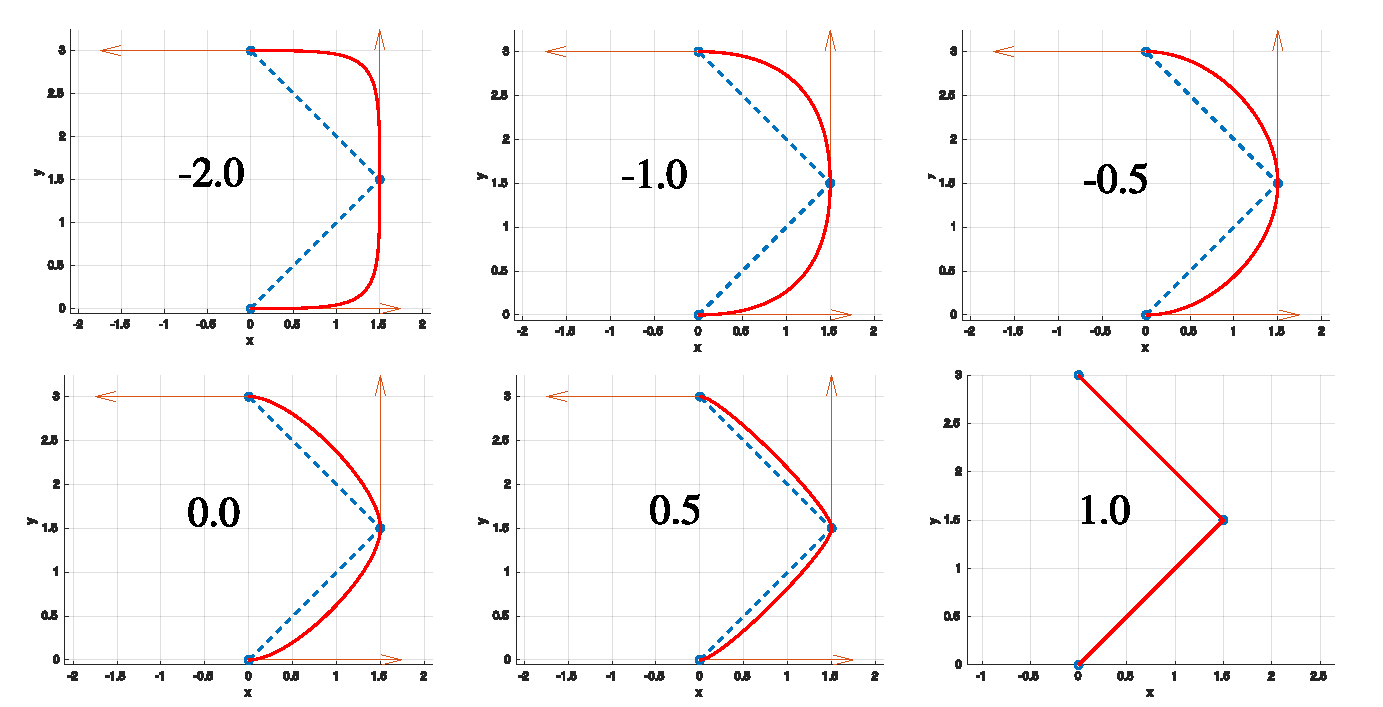
\includegraphics[width=.80\textwidth]{spline_tension}
    \caption{Influence of the \param{tension} parameter on the shape of 
    the spline interpolating points $(0,0)$, $(1.5,1.5)$ $(0,3)$, with 
    prescribed horizontal derivatives at the end points.}
\label{fig:spline_tension}
\end{figure}

\subsection{Limitations and errors in the pointwise definition of a component}
So far, the code has the following limitations:
\begin{itemize}
    \item if \param{mesh\_symmetry = T}, the last section of the component 
    can be joined only if the first section is joined. A workaround is to 
    flip the order of the points and reverse the direction of the reference 
    line, in order to have the first section corresponding to the previously 
    defined last section and viceversa, so that the desired sections are joined. 
    No limitation exists if both the first and last sections belong to the 
    symmetry plane and are joined.
    
    \item it is not possible to join two consecutive \param{spline}s lines. 
    So far, \param{spline}s are meant to join \param{straight} lines or to 
    be the first or last line. However a single spline can be used to join 
    an arbitrary number of points. 
    
    \item it is not possible to define the first or last line as a \param{spline}, 
    without providing the tangent vector at the free end, i.e. the \param{tangent\_vec1} 
    must be provided to the first line, \param{tangent\_vec2} 
    to the last line. spline routines have the capability to 
    treat free ends, with second derivative equal to zero, but 
    some modifications in the pointwise definition of a component 
    are still needed to allow for free ends.
    
\end{itemize}

\subsection{Bodies of Revolution}
\label{subs:Bodies_Revolution}
A simple parametric mesh generation to create bodies of revolution 
is available. With this type of input is possible to generate bodies 
by revolving an user provided profile or cylindrical bodies with smooth 
tapered ends only with parametric inputs. An example of input file 
for this kind of parametric input is available in file 

\begin{inputfile}[frame=single, 
  caption={Boies of revolution geometry definition }, 
  label={file:revolution_example_file.in}]
mesh_file_type = revolution
el_type = p

mesh_symmetry = T
symmetry_point = (/0.0,0.0,0.0/)
symmetry_normal = (/0.0,1.0,0.0/)

mesh_mirror = F
mirror_point = (/0.0,0.0,0.0/)
mirror_normal = (/0.0,1.0,0.0/)

!mesh_file = rev_profile.dat

rev_length = 5.0
rev_nose_radius = 1.0
rev_radius = 0.7
rev_nelem_long = 30
rev_nelem_rev = 10

\end{inputfile}

\begin{itemize}

\item \param{mesh_file_type}: \textit{required:} yes. \textit{multiple:} no. 
\textit{type:} string. 

Use \param{revolution} for bodies of revolution

\item \param{el_type}: \textit{required:} yes. \textit{multiple:} no. 
\textit{type:} character.

    Only \opt{p} for surface panels is supported for bodies of revolution.

\item \param{mesh\_symmetry} \textit{required:} no. \textit{multiple:} no. 
\textit{default:} false. \textit{type:} logical.

Choose to reflect the mesh around a point and a direction. 
Useful to produce full meshes out of symmetrical half models. 
Keeps both the original and the symmetrical part. 

\item \param{symmetry\_point}: \textit{required:} only if 
\param{mesh\_reflection} is true. \textit{multiple:} no. 
\textit{default:} (0.0, 0.0, 0.0). \textit{type:} real array, length 3.

point around which to reflect the mesh.

\item \param{symmetry\_normal}: \textit{required:} only if 
\param{mesh\_reflection} is true. \textit{multiple:} no. 
\textit{default:} (0.0, 1.0, 0.0). \textit{type:} real array, length 3.

Direction in which to reflect the mesh.

\item \param{mesh\_mirror} \textit{required:} no. \textit{multiple:} no. 
\textit{default:} false. \textit{type:} logical.

Choose to mirror the mesh around a point and a direction. Same as 
\param{mesh\_symmetry} but does not keep both the original, i.e. the mesh is not doubled.

\item \param{mirror\_point}: \textit{required:} only if 
\param{mesh\_reflection} is true. \textit{multiple:} no. 
\textit{default:} (0.0, 0.0, 0.0). \textit{type:} real array, length 3.

point around which to mirror the mesh.

\item \param{mirror\_normal}: \textit{required:} only if 
\param{mesh\_reflection} is true. \textit{multiple:} no. 
\textit{default:} (0.0, 1.0, 0.0). \textit{type:} real array, length 3.

Direction in which to mirror the mesh.

\item \param{mesh_file}: \textit{required:} no. \textit{multiple:} no. 
\textit{type:} string.

name of an ascii file containing the point list describing the 
curve or profile to revolve, which will be revolved around the local x axis. 
If the input is present, the rest of the inputs are neglected and the body is 
built revolving the provided profile, otherwise if  \param{mesh_file} is not present, 
the parametric input is employed

\item \param{rev\_length}: \textit{required:} yes if \param{mesh_file} is not present. 
\textit{multiple:} no. \textit{type:} real.

Length of the parametric body of revolution, from tip to tip.

\item \param{rev\_nose\_radius}: \textit{required:} yes if \param{mesh_file} is not present. 
\textit{multiple:} no. \textit{type:} real.

radius of the smooth circular tapering at the ends of the cylindrical body of revolution

\item \param{rev\_radius}: \textit{required:} yes if \param{mesh_file} is not present. 
\textit{multiple:} no. \textit{type:} real.

radius of the central cylindrical section of the body of revolution

\item \param{rev\_nelem\_long}: \textit{required:} yes if \param{mesh_file} is not present. 
\textit{multiple:} no. \textit{type:} integer.

Number of elements in the longitudinal direction of the body of revolution

\item \param{rev\_nelem\_rev}: \textit{required:} yes. \textit{multiple:} no. 
\textit{type:} integer.

Number of elements in the revolution direction. 


\end{itemize}


\section{Trailing Edge}
\label{sec:TrailingEdge}

The trailing edge is the line from which the wake is shed from the geometry elements. 
It is meant to represent the location where the thin vortical layer leaves a lifting 
body when the boundary layer is still attached. In the \DUST \ preprocessor the 
trailing edge is identified geometrically, possibly according to a set of parameters. 

In case of paranetrically generated elements, which represent extruded airfoils, 
the trailing edge is simply generated connecting all the trailing edge of the two 
(or mono) dimensional sections that compose the parametric geometry.

In case of unstructured surface meshes, the preprocessor proceeds by trying to 
geometrically identify the trailing edge in sharp corners between elements. 

Considering the (rather common) possibility that the trailing edges are left open, 
i.e. with element edges not geometrically connected and/or not logically connected 
in the connectivity, first the \DUST preprocessor merges the close nodes and generates 
an alternative connectivity taking into account the new connections. 
This merging is just functional to the definition of the trailing edge, and will 
be discarded after the trailing edge had been identified. To control the merging, 
the parameter \param{tol_se_wing} can be declared in the preprocessor input file, 
to be applied globally, or in each (or some) single geometry input file to be 
applied to a single component. Each pair of nodes separated by a distance lower 
than \param{tol_se_wing} will be merged in this phase.

After merging the mesh the new connectivity will be employed to identify 
the edges belonging to the trailing edge. The edges between two elements 
whose normal vectors are \emph{sufficiently} opposed are marked as trailing 
edge. In particular, the edge connecting the elements $i$ and $j$ is a trailing edge if 
\begin{equation}
    \Vec{n}_i\cdot\Vec{n}_j < \text{\param{inner_product_te}},
\end{equation}
where $\Vec{n}_i,\Vec{n}_j$ are the normal unit vectors of the respective elements.

Moreover during the preprocessing also the direction of the first wake panel 
is decided. During the simulation the whole wake is advected according to the 
velocity generated by the singularities of the bodies and the wake, however the 
first wake panel is geometrically pre-determined and its intensity is implicitly 
solved alongside the rest of the singularities of the body surfaces. The first panel 
starts from the trailing adge and its nodes, and its length is decided during the 
simulation, however the direction alongside it is stretched from the trailing edge 
is determined in the preprocessor. 

If no specific indication is given, the direction of the first implicit wake 
panel is the average of the two edges directions from the upper and lower elements 
connected at the trailing edge node. It is however possible to alter this behaviour 
by setting \param{proj_te} to true. Then the user must provide a direction 
vector with \param{proj_te_vector}, which identifies the direction in which 
to project the first panel direction if \param{proj_te_dir} is \opt{parallel}, 
or is the normal to the plane in which to project the first panel direction if 
\param{proj_te_dir} is \opt{normal}.




\section{Actuator Disks}
\label{sec:ActuatorDisks}
Actuator disks are built employing a parametric input file just as file 
\ref{file:parametric_geo_file.in} but with different parameters, shown in file 
\ref{file:actdisk_geo_file.in} 

\begin{inputfile}[frame=single, caption={actdisk\_geo\_file.in}, 
  label={file:actdisk_geo_file.in}]
mesh_file_type = parametric
el_type = a

radius = 2.5
nstep = 20
axis = 3
traction = 10.0
\end{inputfile}


All the detailed parameters of the geometry input file for parametric actuator disks are:
\begin{itemize}
\item \param{mesh_file_type}: \textit{required:} yes. \textit{multiple:} no. 
\textit{type:} string. 

Use \param{parametric} for parametric geometry.

\item \param{el_type}: \textit{required:} yes. \textit{multiple:} no. 
\textit{type:} character.

type of the elements of the mesh. For actuator disks must be \param{a}

\item \param{radius}: \textit{required:} yes. \textit{multiple:} no. \textit{type:} real.

radius of the actuator disk.

\item \param{nstep}: \textit{required:} yes. \textit{multiple:} no. \textit{type:} integer.

Number of straight segments used to discretize the circle of the actuator disk.

\item \param{axis}: \textit{required:} yes. \textit{multiple:} no. \textit{type:} integer.

Which of the three axis of the reference frame to use as axis of the rotor. 
The reference frame is the one specified for the component in the preprocessor input, 
file \ref{file:dust_pre.in}

\item \param{traction}: \textit{required:} yes. \textit{multiple:} no. \textit{type:} real.

traction of the actuator disk.
\end{itemize}




\chapter{Coupling with a structural software through preCICE}
\section{Introduction}
The communication between DUST and MBDyn is managed by preCICE (Precise Code Interaction Coupling Environment), a coupling library for partitioned multi-physics simulations, originally developed for fluid-structure interaction and conjugate heat transfer simulations.
preCICE offers methods for transient equation coupling, communication means, and data mapping schemes. It is written in C++ and offers additional bindings for C, Fortran, Matlab, and Python.
preCICE~(\url{https://github.com/precice/}) is an open-source software released under the LGPL3 license. 

\section{Compilation}
\textcolor{red}{TODO}
\section{Input Files}
\textcolor{red}{TODO}
\subsection{DUST}
\label{subsec:DUSTpreCICE}
The DUST component input card is enriched of the following parameters:
\begin{itemize}
    \item \param{Coupled} \textit{required:} no. \textit{default:} F. \textit{type:} logical.
    
    Component of a coupled simulation with respect to a structural solver.
    
    \item \param{CouplingType} \textit{required:} yes. \textit{type:} string. 
    Type of the coupling:
    \begin{itemize}
        \item \opt{rigid}: rigid component and node 
        \item \opt{rbf}: Generic DUST component and node coupling
    \end{itemize}
    Although three different types of are implemented, the most general one is the \opt{rbf} since it can manage all DUST components and can be coupled with both rigid and flexible elements.  
   
   \item \param{CouplingNode} \textit{required:} no. \textit{type:} real array, length 3. \textit{default:} (0.0, 0.0, 0.0)
   
   Node for \opt{rigid} coupling in the reference configuration (x, y, z).
   
   \item \param{CouplingNodeFile} \textit{required:} yes. \textit{type:} string. 
   
   File containing the nodes for FSI (fluid structure interaction). It is required for \opt{rbf} coupling. 
   
   \item \param{CouplingNodeOrientation} \textit{required:} no. \textit{type:} real array, length 3. \textit{default:} (1.,0.,0., 0.,1.,0., 0.,0.,1.)
   
   Orientation of the node for rigid coupling. This array contains the local components (in the local reference frame of the geometrical           component) of the unit vectors of the coupling node reference frame. In the \opt{rbf} frame indicates the rotation matrix from the structural component to the DUST component reference frame. 
   
\end{itemize}
\subsection{preCICE XML}
preCICE needs to be configured at runtime via an \texttt{xml} file, typically named \texttt{precice-config.xml}. Here, you specify which solvers participate in the coupled simulation, which coupling data values they exchange, which fixed-point acceleration and many other things.

First of all, the fields exposed to communication between the two solvers are declared.
\begin{lstlisting}[language=XML]
<?xml version="1.0"?>

<precice-configuration>

  <solver-interface dimensions="3">

    <!-- === Data =========================================== -->
    
    <data:vector name="Position" />
    <data:vector name="Rotation" />
    <data:vector name="Velocity" />
    <data:vector name="AngularVelocity" />
    <data:vector name="Force" />
    <data:vector name="Moment" />
\end{lstlisting}  

Here follows the definition of the two meshes, for each of which it is declared which data among the declared before are used.
In this case, both DUST and MBDyn use all the exposed fields.
\begin{lstlisting}[language=XML]
    <!-- === Mesh =========================================== -->
    <mesh name="MBDynNodes">
      <use-data name="Position" />
      <use-data name="Rotation" />
      <use-data name="Velocity" />
      <use-data name="AngularVelocity" />
      <use-data name="Force" />
      <use-data name="Moment" />
    </mesh>

    <mesh name="dust_mesh">
      <use-data name="Position" />
      <use-data name="Rotation" />
      <use-data name="Velocity" />
      <use-data name="AngularVelocity" />
      <use-data name="Force" />
      <use-data name="Moment" />
    </mesh>
\end{lstlisting} 

In this part are declared the two participants, MBDyn and DUST. For each participant it is indicated which field is received (\texttt{read-data}) and which is sent (\texttt{write-data}). Considering DUST, this receives the kinematic variables and sends the loads. 
\begin{lstlisting}[language=XML]
    <!-- === Participants =================================== -->
    <participant name="MBDyn">
      <use-mesh   name="MBDynNodes" provide="yes"/>
      <write-data name="Position"        mesh="MBDynNodes" />
      <write-data name="Rotation"        mesh="MBDynNodes" />
      <write-data name="Velocity"        mesh="MBDynNodes" />
      <write-data name="AngularVelocity" mesh="MBDynNodes" />
      <read-data  name="Force"           mesh="MBDynNodes" />
      <read-data  name="Moment"          mesh="MBDynNodes" />
    </participant>

    <participant name="dust">
      <use-mesh   name="dust_mesh"  provide="yes" />
      <use-mesh   name="MBDynNodes" from="MBDyn" />
      <write-data name="Force"           mesh="dust_mesh" />
      <write-data name="Moment"          mesh="dust_mesh" />
      <read-data  name="Position"        mesh="dust_mesh" />
      <read-data  name="Rotation"        mesh="dust_mesh" />
      <read-data  name="Velocity"        mesh="dust_mesh" />
      <read-data  name="AngularVelocity" mesh="dust_mesh" />
      <mapping:nearest-neighbor direction="read"  from="MBDynNodes" to="dust_mesh"
        constraint="consistent" />
      <mapping:nearest-neighbor direction="write" from="dust_mesh"  to="MBDynNodes"
        constraint="conservative" />
    </participant>
\end{lstlisting}

For each two participants that should exchange data, you have to define an m2n communication. 
This establishes an m2n (i.e. parallel, from the M processes of the one participant to the N processes of the other) communication channel based on TCP/IP sockets between MBDyn and DUST.
\begin{lstlisting}[language=XML]
    <!-- === Communication ================================== -->
    <m2n:sockets exchange-directory="./../" from="MBDyn" to="dust"/>
\end{lstlisting}

A coupling scheme can be either serial or parallel and either explicit or implicit. Serial refers to the staggered execution of one participant after the other where the first participant is computed before the second one. With an explicit scheme, both participants are only executed once per time window. With an implicit scheme, the participants are executed multiple times until convergence.

The \texttt{max-time value} field indicates the maximum time (end time) for the coupled simulation  (NOTE: actually the final time is the shorter between this and the final time set in DUST and in the MBDyn input).

With \texttt{time-window-size value}, you can define the coupling time window (=coupling time step) size. If a participant uses a smaller one, it will subcycle until this window size is reached. 
Setting it equal to -1, it is set according to a specific \texttt{method}, here taking the value form the first participant MBDyn.

To control the number of sub-iterations within an implicit coupling loop, you can specify the maximum number of iterations, \texttt{max-iterations} and you can specify one or several convergence measures:
\begin{itemize}
    \item \texttt{relative-convergence-measure} for a relative criterion
    \item \texttt{absolute-convergence-measure} for an absolute criterion
    \item \texttt{min-iteration-convergence-measure} to require a minimum of iterations
\end{itemize}

\begin{lstlisting}[language=XML]
    <!-- === Coupling scheme ================================ -->
    <coupling-scheme:serial-implicit>
      <participants first="MBDyn" second="dust" />
      <max-time value="100.0" />
      <time-window-size value="-1" valid-digits="10" method="first-participant" />
      <exchange data="Position"        from="MBDyn" mesh="MBDynNodes" to="dust" />
      <exchange data="Rotation"        from="MBDyn" mesh="MBDynNodes" to="dust" />
      <exchange data="Velocity"        from="MBDyn" mesh="MBDynNodes" to="dust" />
      <exchange data="AngularVelocity" from="MBDyn" mesh="MBDynNodes" to="dust" />
      <exchange data="Force"           from="dust"  mesh="MBDynNodes" to="MBDyn" />
      <exchange data="Moment"          from="dust"  mesh="MBDynNodes" to="MBDyn" />
      <max-iterations value="60"/>
      <absolute-convergence-measure limit="1.0e-4" data="Position" mesh="MBDynNodes" />
      <absolute-convergence-measure limit="1.0e-3" data="Rotation" mesh="MBDynNodes" />
      <absolute-convergence-measure limit="1.0e-3" data="Velocity" mesh="MBDynNodes" />
      <absolute-convergence-measure limit="1.0e-3" data="AngularVelocity" mesh="MBDynNodes" /> 
\end{lstlisting}

Mathematically, implicit coupling schemes lead to fixed-point equations at the coupling interface. A pure implicit coupling without acceleration corresponds to a simple fixed-point iteration, which still has the same stability issues as an explicit coupling. We need acceleration techniques to stabilize and accelerate the fixed-point iteration. 
In preCICE, three different types of acceleration can be configured: constant (\texttt{constant} under-relaxation), \texttt{aitken} (adaptive under-relaxation), and various quasi-Newton variants (\texttt{IQN-ILS} aka. Anderson acceleration, \texttt{IQN-IMVJ} aka. generalized Broyden).
\begin{lstlisting}[language=XML]
      <acceleration:aitken>
        <data name="Force" mesh="MBDynNodes"/>
        <initial-relaxation value="0.1"/>
      </acceleration:aitken>		
    </coupling-scheme:serial-implicit>

  </solver-interface>

</precice-configuration>
\end{lstlisting}

For more details, see \url{https://precice.org}.
\subsection{MBDyn external force}
The aerodynamic loads computed by DUST are introduced in the MBDyn model as an external structural force acting on some nodes.

\section{Coupling workflow}
In this section the workflow to build a coupled model will be deeply explained considering the cases of a generic aircraft with a fuselage (modelled as rigid body) and a flexible wing, and the case of flexible three bladed rotor. 
Both examples will use the \opt{rbf} coupling type. 

\subsection{Wing with Control Surfaces}
Let consider the case of a symmetric wing. According to MBDyn manual, it is easier to define the beam axis oriented with the local $x$. Let define the angles $\lambda$, $\delta$, $\theta$ as the sweep, dihedral and twist angle. In order to pass from the global or wind axis frame of reference to the local beam axis the following rotation matrix are used: 

\begin{itemize}
    \item Rotation matrix from the DUST reference frame to the MBDyn reference frame:
    \begin{equation}
        \mathbf{R}_{b} = 
        \begin{bmatrix}
            0 & 1 & 0\\
            -1 & 0 & 0\\
            0 & 0 & 1
        \end{bmatrix}
        \label{eq:rotbeam}
    \end{equation}

    \item Twist rotation of the MBDyn node around the beam axis $x$. 
    \begin{equation}
        \mathbf{R}_{\theta} = 
        \begin{bmatrix}
            \cos \theta & 0 & \sin\theta\\ 
            0 & 1 & 0\\ 
            -\sin\theta & 0 & \cos\theta
        \end{bmatrix}
        \label{eq:rottwist}
    \end{equation}
    
    \item Sweep rotation of the MBDyn node. The sweep is taken positive for a rotation about $-z$. 
    \begin{equation}
        \mathbf{R}_{\lambda} = 
        \begin{bmatrix}
            \cos\lambda & -\sin\lambda & 0\\ 
            \sin\lambda & \cos\lambda & 0\\ 
            0 & 0 & 1 
        \end{bmatrix}
        \label{eq:rotsweep}
    \end{equation}
    
    \item Dihedral rotation of the MBDyn node. 
    \begin{equation}
        \mathbf{R}_{\delta} = 
        \begin{bmatrix}
            1 & 0 & 0\\ 
            0 & \cos\delta & \sin\delta\\ 
            0 & -\sin\delta & \cos\delta 
        \end{bmatrix}
        \label{eq:rotdih}
    \end{equation}
\end{itemize}



Generic rotation matrix for a right wing: 
\begin{align*}
    \mathbf{R}_{\text{right}}& =   \mathbf{R}_{b}\mathbf{R}_{\theta}\mathbf{R}_{\lambda}\mathbf{R}_{\delta} = \\
    &=\begin{bmatrix}
    \sin\lambda  & 
    \cos\delta \,\cos\lambda  & 
    \cos\lambda \,\sin\delta \\
    -\cos\lambda \,\cos\theta  & 
    \sin\delta \,\sin\theta +\cos\delta \,\cos\theta \,\sin\lambda  & 
    \sin\delta \,\cos\theta \,\sin\lambda -\cos\delta \,\sin\theta \\ 
    -\cos\lambda \,\sin\theta  & 
    \cos\delta \,\sin\lambda \,\sin\theta -\sin\delta \,\cos\theta  & 
    \cos\delta \,\cos\theta +\sin\delta \,\sin\lambda \,\sin\theta
    \end{bmatrix}
\end{align*}

Generic rotation matrix for a left wing: 
\begin{align*}
    \mathbf{R}_{\text{left}}&=   \mathbf{R}_{b}\mathbf{R}_{\theta}\mathbf{R}_{\lambda}^T\mathbf{R}_{\delta}^T =\\
    &=\begin{bmatrix} 
    -\sin\lambda  &
    \cos\delta \,\cos\lambda  &
    -\cos\lambda \,\sin\delta \\
    -\cos\lambda \,\cos\theta  & 
    -\sin\delta \,\sin\theta -\cos\delta \,\cos\theta \,\sin\lambda  & 
    \sin\delta \,\cos\theta \,\sin\lambda -\cos\delta \,\sin\theta \\ 
    -\cos\lambda \,\sin\theta  & 
    \sin\delta \,\cos\theta -\cos\delta \,\sin\lambda \,\sin\theta  &
    \cos\delta \,\cos\theta +\sin\delta \,\sin\lambda \,\sin\theta  
    \end{bmatrix}
\end{align*}

All these rotations are intended to rotate back the structural component in the DUST component reference frame. When this procedure is performed, then the aerodynamic mesh can be constructed as a normal DUST parametric mesh. 
\textcolor{red}{TODO}

%\subsection{Flexible Rotor} 
%\section{Example: Rigid Mesh}

\chapter{DUST solver}

The DUST solver is the main executable of DUST, and its aim is to run 
the actual simulation and obtain the required full solution to the problem. 

As the other executable it is run by simply invoking the executable \texttt{dust} with the correct input file as command argument.
\begin{command}[caption={Solver command looking for input file 
    \texttt{input\_file\_name.in}}]
    dust input_file_name.in
\end{command}

If no command argument is provided the solver looks for a default input file, \texttt{dust.in}. 
\begin{command}[caption={Solver command looking for 
default input file \texttt{dust.in}}]
    dust
\end{command}

The solver requires, among other inputs, the geometry file result of the preprocessor. 
If such file is not found the solver attempts to run the preprocessor by executing 
the preprocessor with default input file (command \ref{command:dus_pre_default}). 

\section{Input file}
\label{sec:Solver_InputFile}

The input file which should be provided to the solver is used to set all t
he parameters required for the execution of the simulation, 
from execution options, time parameters to the wake and model 
settings. 

An example of input file for the solver is presented in file \ref{file:dust.in}

\begin{inputfile}[frame=single, caption={dust.in}, label={file:dust.in}]

! --- execution parameters ---
basename = sim_01
basename_debug = sim_01_debug
debug_level = 3

! --- time parameters ---
tstart = 0.0
tend = 10.0
timesteps = 20
!dt = 0.5
dt_out = 2.0
dt_debug_out = 1.0
output_start = F
output_detailed_geo = T 

! --- restart parameters ---
restart_from_file = F
restart_file = prev_solution_0021.h5
reset_time = F

! --- input files ---
reference_file = References.in
geometry_file = geo_file.h5

! --- stream parameters ---
u_inf = (/1.0, 0.0, 0.0/)
u_ref = 1.0
P_inf = 1.0
rho_inf = 1.0
a_inf = 340.0
mu_inf = 0.00001

! --- wake parameters ---
n_wake_panels = 4
n_wake_particles = 10000
particles_box_min = (/-10.0, -10.0, -10.0/)
particles_box_max = (/10.0, 10.0, 10.0/)
implicit_panel_scale = 0.3
implicit_panel_min_vel = 1.0e-8
rigid_wake = F
rigid_wake_vel = (/1.0, 0.0, 0.0/)
join_te = F
join_te_factor = 1.0

! --- model parameters ---
far_field_ratio_doublet = 10.0
far_field_ratio_source = 10.0
doublet_threshold = 1.0e-6
rankine_rad = 0.1
vortex_rad = 0.1
k_vortex_rad = 1.0
cutoff_rad = 0.001

! --- additional models to use ---
vortstretch = T
vortstretch_from_elems = F
diffusion = T
turbulent_viscosity = F
penetration_avoidance = F
penetration_avoidance_check_radius = 5.0
penetration_avoidance_element_radius = 1.5
divergence_filtering = T
filter_time_scale = 40.0
fmm = T
fmm_panels = F
viscosity_effects = F
particles_redistribution = F
particles_redistribution_ratio = 3.0
octree_level_solid = 4
turbulent_viscosity = F
HCAS = F
HCAS_time = 4.0
HCAS_velocity = (/2.0, 0.0, 0.0/)

! --- Fast multipole parameters ---
box_length = 10.0
n_box = (/2, 2, 2/)
octree_origin = (/-10.0, -10.0, -10.0/)
n_octree_levels = 6
min_octree_part =  10
multipole_degree = 2
dyn_layers = F
nmax_octree_levels = 7
leaves_time_ratio = 3.0

! --- Lifting Lines parameters ---
ll_solver = GammaMethod
ll_reynolds_corrections = F
ll_reynolds_corrections_nfact = 0.2
ll_max_iter = 100
ll_tol = 1.0e-6
ll_damp = 5.0
ll_stall_regularisation = T
ll_stall_regularisation_nelems = 1
ll_stall_regularizations_niters = 1
ll_stall_regularization_alpha_stall = 15
ll_artificial_viscosity = 0.0
ll_artificial_viscosity_adaptive = F
ll_artificial_viscosity_adaptive_alpha = 15
ll_artificial_viscosity_adaptive_dalpha = 3
ll_loads_avl = F

! --- Vortex Lattice Correction ---
vl_tol = 1.0e-4
vl_relax = 0.3
vl_maxiter = 100
vl_start_step = 0
vl_dynstall = F
aitken_relaxation = T 

\end{inputfile}

The details of each parameter are:
\begin{itemize}
\item \param{basename}: \textit{required:} yes. \textit{multiple:} no. \textit{type:} string.

The base name of the simulation and will be the prefix of the output files. 
Can be a complete path leading to the location in which to store the results. 

\item \param{basename\_debug}: \textit{required:} no. \textit{multiple:} no. 
\textit{default:} \param{basename} \textit{type:} string.

The base name of the debug output. It is especially useful to direct the 
debug output to a different location than the standard output. 
The amount of (if any) debug output is controlled by \param{debug\_level}.

\item \param{debug\_level}: \textit{required:} no. \textit{multiple:} no. 
\textit{default:} 1\textit{type:} integer.

A parameter controlling the verbosity (both in terms of standard output and files output) 
of the simulation. A smaller value leads to fewer output, with 0 being a silent simulation, 
while values higher of 10 lead to debug files to be produced. 
A value of 3 is a balanced value to obtain a reasonable amount of informations 
on the simulation. 

WARNING: the present feature tends to evolve rapidly during the development. 
Values higher than 10 may lead to unexpected behaviours. 


\item \param{tstart}: \textit{required:} yes. \textit{multiple:} no. \textit{type:} real.

The start time of the simulation.

\item \param{tend}: \textit{required:} yes. \textit{multiple:} no. \textit{type:} real.

The end time of the simulation.

\item \param{timesteps}: \textit{required:} yes if \param{dt} not set, forbidden if set. 
\textit{multiple:} no. \textit{type:} integer.

The number of timesteps for the simulation. Note that during the simulation a number 
of timesteps equal to \param{timesteps}+1 will be displayed, because the starting step 
is counted too. 

\item \param{dt}: \textit{required:} yes if \param{timesteps} not set, forbidden if set. 
\textit{multiple:} no. \textit{type:} real.

The time step length.

\item \param{dt\_out}: \textit{required:} yes. \textit{multiple:} no. \textit{type:} real.

Time interval of solution output.

\item \param{dt\_debug\_out}: \textit{required:} no. \textit{multiple:} no. \textit{default:} 
\param{dt\_out}. \textit{type:} real.

Time interval of debug output, if \param{debug\_level} is set high enough to write debug 
files.


\item \param{output\_start}: \textit{required:} no. \textit{multiple:} no. 
\textit{default} False. \textit{type:} logical.

Output the first iteration. Since it is an implicit solver, the first calculation happens 
at $t_0$ before any time interval has passed, if set to True output the first result.

\item \param{output\_detailed\_geo}: \textit{required:} no. \textit{multiple:} no. 
\textit{default} False. \textit{type:} logical.

Output additional geometry information in the result files. Makes the result files 
easier to interpret by third party software, however makes the result files slightly 
bigger and output slightly slower.

\item \param{restart\_from\_file}: \textit{required:} no. \textit{multiple:} no. 
\textit{default:} False. \textit{type:} logical.

Restart the simulation from a previous result.


\item \param{restart\_file}: \textit{required:} yes if \param{restart\_from\_file} 
is true. \textit{multiple:} no. \textit{type:} string.

name of the solution file from which to restart the simulation.

Note: when reloading a certain result, the solver will attempt to load also the 
relative geometry file in the same location, as discussed in \ref{sec:Solver_Output_Files}. 
If such geometry file is not provided the solver, as in the case of standard starting, 
will attempt to generate such file with the default preprocessor input. Beware that in 
this case, if the geometry of the results from which the solver is starting was generated 
from another geometry input this could lead to unexpected behaviour.


\item \param{reset\_time}: \textit{required:} no. \textit{multiple:} no. \textit{default:} 
False. \textit{type:} logical.

If set to true, when restarting from a previous result, the time will be set as the 
\param{tstart} from the input file. If set to false, the time will be set as the one 
from the result file loaded. This is delicate since the movement of the reference 
frames is based on the current time in the simulation, and if reset the time could 
lead to a position of the geometry different from the one in the loaded result file.


\item \param{reference_file}: \textit{required:} yes. \textit{multiple:} no. 
\textit{type:} string.

name of the file containing the definition of the reference frames employed 
in the simulation.


\item \param{geometry_file}: \textit{required:} yes. \textit{multiple:} no. 
\textit{type:} string.

name of the file containing the geometry definition, generated by the preprocessor


\item \param{u\_inf}: \textit{required:} no. \textit{multiple:} no. 
\textit{default:} (/1.0, 0.0, 0.0/) \textit{type:} real array of length 3.

Free stream velocity vector.

\item \param{u\_ref}: \textit{required:} no. \textit{multiple:} no. 
\textit{default:} $|\text{\param{u\_inf}}|$ \textit{type:} real.

Reference velocity. Usually is safe not to set anything and use the norm 
of the free stream velocity, however in hover flight conditions it is useful 
to set a non zero reference velocity (e.g. the blade tip velocity)


\item \param{gust}: \textit{required:} no. \textit{multiple:} no. 
\textit{default:} F \textit{type:} logical.

\begin{itemize}
    
    \item \param{gust_type}: \textit{required:} no. \textit{multiple:} no. \textit{default:} AMC \textit{type:} string.
    
    Select the gust type: \opt{ACM} or \opt{linear}.
    \begin{equation}
        \vec{s} = -\sum \big[\vec{x} - \big(\vec{O} + U_{des}\vec{v}(t-\tau)\big)\vec]\vec{v}
    \end{equation}
        
    \begin{equation}
        \vec{U} = \vec{U}  + \dfrac{U_{des}}{2}\bigg(1-\cos{\frac{\pi s}{H}}\bigg)    
    \end{equation}
    
    \item \param{gust_origin}: \textit{required:} yes. \textit{multiple:} no. 
    \textit{type:} real array of length 3.
    
    $\vec{0}$: Position of the point  whose airstream velocity is being computed. 
    
    \item \param{gust_front_direction}: \textit{required:} yes. \textit{multiple:} no. 
    \textit{type:} real array of length 3.
    
    $\vec{v}$: Unit vector that defines the direction of propagation of the front. 
    
    \item \param{gust_front_speed}: \textit{required:} yes. \textit{multiple:} no. 
    \textit{type:} real.
    
    Velocity of propagation of the front in direction 
    \param{gust_front_direction}
    
    \item \param{gust_u_des}: \textit{required:} yes. \textit{multiple:} no. 
    \textit{type:} real.
    
    $U_{des}$: gust amplitude. 
    
    \item \param{gust_perturbation_direction}: \textit{required:} no. 
    \textit{multiple:} no. \textit{default:} (/0.0, 0.0, 1.0/) 
    \textit{type:} real array of length 3.
    
    Unit vector that defines the direction of the velocity perturbation
    
    \item \param{gust_gradient}: \textit{required:} no. \textit{multiple:} yes. 
    \textit{type:} real.
    
    H: gust wave length. 
    
    \item \param{gust_start_time}: \textit{required:} no. \textit{multiple:} no. 
    \textit{default:} 0.0 \textit{type:} real.
    
    $\tau$: Time at which the gust starts. 
\end{itemize}

\item \param{P\_inf}: \textit{required:} no. \textit{multiple:} no. 
\textit{default:} 101325.0 \textit{type:} real.

Free stream pressure.

\item \param{a\_inf}: \textit{required:} no. \textit{multiple:} no. 
\textit{default:} 340.0 \textit{type:} real.

Free stream sound speed. For lifting lines and compressibility corrections.


\item \param{mu\_inf}: \textit{required:} no. \textit{multiple:} no. 
\textit{default:} 0.000018 \textit{type:} real.

Free stream dynamical viscosity. For lifting lines and viscosity corrections.

\item \param{rho\_inf}: \textit{required:} no. \textit{multiple:} no. 
\textit{default:} 1.225 \textit{type:} real.

Free stream density.

\item \param{n\_wake\_panels}: \textit{required:} no. \textit{multiple:} no. 
\textit{default:} 1 \textit{type:} integer.

Number of panel wake rows before converting the wake to vortex particles.


\item \param{n\_wake\_particles}: \textit{required:} no. \textit{multiple:} no. 
\textit{default:} 10000 \textit{type:} integer.

Number of maximum vortex particles in the wake. If the limit is reached the simulation is stopped, but can be restarted from last save with a higher value of the parameter. 


\item \param{particles\_box\_min}: \textit{required:} no. \textit{multiple:} no. 
\textit{default:} (/-10.0, -10.0, -10.0/) \textit{type:} real array of length 3.

Minimum coordinates (in the base reference frame) of the box containing the vortex 
particles. If the particles get outside the box are cancelled.

\item \param{particles\_box\_max}: \textit{required:} no. \textit{multiple:} no. 
\textit{default:} (/10.0, 10.0, 10.0/) \textit{type:} real array of length 3.

Maximum coordinates (in the base reference frame) of the box containing the vortex 
particles. If the particles get outside the box are cancelled.

\item \param{implicit_panel_scale}: \textit{required:} no. \textit{multiple:} no. 
\textit{default:} 0.3 \textit{type:} real.

Scaling of the first panel of the wake, the implicit one which enforces the Kutta 
condition. The first panel geometry is not dictated by the advection of its 
vertices as for the other ones, but the first row of points come from the geometry, 
while the second row is calculated by local velocity and timestep, 
scaled by the \param{implicit_panel_scale} parameter.


\item \param{implicit_panel_min_vel}: \textit{required:} no. \textit{multiple:} no. 
\textit{default:} 1.0e-8 \textit{type:} real.

When the free stream velocity and body motions do not create a sufficiently high 
local velocity at the trailing edge, the first panel might turn out of zero length. 
To avoid this, when the trailing edge local velocity is below 
\param{implicit_panel_min_vel} a fixed length of the panel is imposed.

\item \param{rigid\_wake}: \textit{required:} no. \textit{multiple:} no. 
\textit{default:} False \textit{type:} logical.

Impose a wake which is evolved rigidly according to a prescribed global 
velocity rather than the local velocity field. Works for both panels and 
particles.

\item \param{rigid\_wake\_vel}: \textit{required:} yes if \param{rigid\_wake} is True. 
\textit{multiple:} no. \textit{type:} real array of length 3.

Velocity to impose to the rigid wake.

\item \param{join\_te}: \textit{required:} no. \textit{multiple:} no. 
\textit{default:} False. \textit{type:} logical.

Employ trailing edge joining for close trailing edges.

\item \param{join\_te\_factor}: \textit{required:} no. \textit{multiple:} no. 
\textit{default:} 1.0. \textit{type:} real.

If employing joining of trailing edges, the trailing edges which are closer than 
\param{join\_te\_factor} times the length of the adjacent trailing edge elements 
will be joined. 

\item \param{far_field_ratio_doublet}: \textit{required:} no. \textit{multiple:} no. 
\textit{default:} 10.0 \textit{type:} real.

Ratio with respect to element length to set the thresholds for far field approximation. 
When evaluating the influence of the doublets of an element, 
if the evaluation point is distant more than \param{far_field_ratio_doublet} 
times the characteristic length of the element, simplified cheaper far field 
approximated formulae are employed instead of the standard ones. 
The characteristic length of the element is taken as the maximum 
length of all the element edges.

\item \param{far_field_ratio_source}: \textit{required:} no. 
\textit{multiple:} no. \textit{default:} 10.0 \textit{type:} real.

As for \param{far_field_ratio_doublet} determines the threshold 
after which far field approximations are employed, just for sources. 
Applies only to three dimensional surface panels. 

\item \param{doublet_threshold}: \textit{required:} no. \textit{multiple:} no. 
\textit{default:} 1.0e-6 \textit{type:} real.

Parameter which sets the distance threshold under which the evaluation point, 
with respect to a panel, is considered inside the plane of the panel.

\item \param{rankine_rad}: \textit{required:} no. \textit{multiple:} no. 
\textit{default:} 0.1 \textit{type:} real.

Parameter which sets the radius under which the Rankine approximation of 
vortexes cores is employed. Used for aerodynamic elements and panels 
(i.e. everything except vortex particles)

\item \param{vortex_rad}: \textit{required:} no. \textit{multiple:} no. 
\textit{default:} 0.1 \textit{type:} real.

Parameter which uniformly sets the radius of the vortex particles, only used if \param{k_vortex_rad} is disabled.

\item \param{k_vortex_rad}: \textit{required:} no. \textit{multiple:} no. \textit{default:} 1.0 \textit{type:} real.

Coefficient for the automatic computation of the radius of each vortex particle; set a negative number to disable the feature and revert to uniform vortex radius. 

\item \param{cutoff_rad}: \textit{required:} no. \textit{multiple:} no. 
\textit{default:} 0.001 \textit{type:} real. 

Parameter which sets the radius under which the vortexes interaction is completely set to zero.

\item \param{vortstretch}: \textit{required:} no. \textit{multiple:} no. 
\textit{default:} T \textit{type:} logical.

Calculate the evolution of vorticity of the particles considering the 
vortex stretching

\item \param{vortstretch_from_elems}: \textit{required:} no. 
\textit{multiple:} no. \textit{default:} F \textit{type:} logical.

Compute also the contribution to the vortex stretching of the particles 
due to the model elements. 

\item \param{diffusion}: \textit{required:} no. \textit{multiple:} no. 
\textit{default:} T \textit{type:} logical.

Calculate the evolution of vorticity of the particles considering the vorticity diffusion

\item \param{turbulent_viscosity}: \textit{required:} no. \textit{multiple:} no. 
\textit{default:} F \textit{type:} logical.

Introduce additional turbulent viscosity (Smagorinsky style) to the vorticity 
diffusion term. Working only when \param{fmm} is turned on. Still experimental feature. 

\item \param{penetration_avoidance}: \textit{required:} no. \textit{multiple:} no. 
\textit{default:} F \textit{type:} logical.

Apply the penetration avoidance algorithm to avoid the penetration of particles 
inside the solid bodies.

\item \param{penetration_avoidance_check_radius}: \textit{required:} no. 
\textit{multiple:} no. \textit{default:} 5.0 \textit{type:} real.

radius multiplication factor of the check radius. All the particles within a 
distance $d\leq P_r U_{ref} \Delta t$ from each element are checked for 
potential penetration, where $P_r$ is the multiplication factor. 
A bigger factor minimizes the risk of penetration of extremely fast particles, 
but affects the performance. 

\item \param{penetration_avoidance_element_radius}: \textit{required:} no. 
\textit{multiple:} no. \textit{default:} 1.5 \textit{type:} real.

Surface correction element radius multiplication factor.
The velocity of the particles is corrected to avoid penetration through a 
particular element if the particle hits the surface within a distance 
(tangent to the surface) $d_t \leq P_e \max{l_i} \frac{\sqrt{2}}{2}$ 
from the element centre, where $l_i$ are the lenght of the element sides 
and $P_e$ is the factor. 
A bigger factor leads to a potentially higher level of correction 
(concurrent correction from different neighbouring elements) 
while a smaller factor may let some particles slip through the surface. 

\item \param{divergence_filtering}: \textit{required:} no. \textit{multiple:} no. 
\textit{default:} T \textit{type:} logical.

Employ the divergence filtering to keep the vorticity field divergence-free. 

\item \param{filter_time_scale}: \textit{required:} no. \textit{multiple:} no. 
\textit{default:} 40.0 \textit{type:} real.

Timescale of the time filter to filter the divergence. 
The input is not the actual timescale but the number of simulation timesteps 
of which the timescale is consisting. 

\item \param{fmm}: \textit{required:} no. \textit{multiple:} no. \textit{default:} T 
\textit{type:} logical.

Use the fast multipole method for particles evolution.

\item \param{fmm_panels}: \textit{required:} no. \textit{multiple:} no. 
\textit{default:} F \textit{type:} logical.

Use the fast multipole method also to compute interactions 
of the particles on the solid bodies panels.

\item \param{viscosity_effects}: \textit{required:} no. \textit{multiple:} no. 
\textit{default:} F \textit{type:} logical.

Take into account viscosity effects on the geometry surface: 
enables the release of vortex particles from different points 
on the geometry surface. Experimental feature, still in development.

\item \param{particles_redistribution}: \textit{required:} no. 
\textit{multiple:} no. \textit{default:} F \textit{type:} logical.

Redistribute the particles having a small intensity to the neighbouring ones. 
Active only if \param{fmm} is active, otherwise ignored. Redistributed particles 
are then ereased to reduce the total number of particles.

\item \param{particles_redistribution_ratio}: \textit{required:} no. 
\textit{multiple:} no. \textit{default:} 3.0 \textit{type:} real.

When employing \param{particles_redistribution}, each particle of intensity 
$|\vec{\alpha}_i|$ will be redistributed to the other particles contained 
in the octree leaf cell if $|\vec{\alpha}_i| r < \alpha_{ave}$ where $r$ is 
\param{particles_redistribution_ratio} and $\alpha_{ave}$ is the average 
intensity of the particles inside the cell.

\item \param{octree_level_solid}: \textit{required:} yes, if 
\param{particles_redistribution} is true. \textit{multiple:} no. 
\textit{type:} integer.

When employing \param{particles_redistribution}, the particles too near 
to a solid boundary are not redistributed to reduce the error induced by 
the redistribution on the solution on solid surfaces. The octree cells at 
level \param{octree_level_solid} containing a panel (SP, VL or LL) are marked 
as containing a solid boudary, as well as all their neighbour at that level. 
All the children of cells containing a solid boundary are marked as containing 
a solid boundary. In the cells containing a solid boundary the redistribution 
is not performed.

For this reason, a small \param{octree_level_solid} approaching 1 will lead 
to a wide zone around solid bodies in which redistribution does not occur, 
while a \param{octree_level_solid} approaching \param{n_octree_levels} leads 
to redistribution to be performed in areas up to close to the solid bodies.

\item \param{turbulent_viscosity}: \textit{required:} no. \textit{multiple:} no. 
\textit{default:} F \textit{type:} logical.

Employ an additional turbulent viscosity, using a Smagorinsky-like model to 
take into account the dissipation of energy in turbulent conditions towards 
small, not resolved turbulent scales. It works only in an octree environment, 
so when \param{fmm} is active.

\item \param{HCAS}: \textit{required:} no. \textit{multiple:} no. 
\textit{default:} F \textit{type:} logical.

Hover Convergence Augmentation System. An additional velocity is applied 
to the particles in the wake to let the particles generated in the transient 
condition at the start to be pushed faster outside the domain, and reach 
stationary conditions faster. The velocity defined by \param{HCAS\_velocity} 
is applied full only at the beginning of the simulation, and is then decreased 
linearly in \param{HCAS\_time}. After \param{HCAS\_time} after the simulation 
start the additional velocity is not applied anymore and the simulation carries 
on without tampering. 

\item \param{HCAS\_time}: \textit{required:} yes if \param{HCAS} is true. 
\textit{multiple:} no. \textit{type:} real.

Duration of HCAS application

\item \param{HCAS\_velocity}: \textit{required:} yes if \param{HCAS} is true. 
\textit{multiple:} no. \textit{type:} real array of length 3.

Velocity to apply to the particles during the HCAS use. 

\item \param{box_length}: \textit{required:} yes if \param{fmm} is true. 
\textit{multiple:} no. \textit{type:} real.

Length of the level 1 cubic boxes composing the octree. See figure 
\ref{fig:boxes1} for a graphic explanation.

\item \param{n_box}: \textit{required:} yes if \param{fmm} is true. 
\textit{multiple:} no. \textit{type:} integer array of length 3.

Number of base level 1 cubic boxes in each spatial direction. See figure 
\ref{fig:boxes1} for a graphic explanation.

\item \param{octree_origin}: \textit{required:} yes if \param{fmm} is true. 
\textit{multiple:} no. \textit{type:} real array of length 3. 

origin of the octree. Starting from the origin, the octree mesh extends in 
each direction of \param{n_box} times \param{box_length}. 
See figure \ref{fig:boxes1} for a graphic explanation.

\item \param{n_octree_levels}: \textit{required:} yes if \param{fmm} is true. 
\textit{multiple:} no. \textit{type:} integer.

Number of levels in  which the base boxes are divided. At each level 
the upper level boxes are divided into eight half sized boxes. 

\item \param{min_octree_part}: \textit{required:} yes if \param{fmm} is true. 
\textit{multiple:} no. \textit{type:} integer.

Minimum number of particles contained in an octree box in order to consider 
it a leaf (lowest level box). If not enough particles are contained in a 
box, the box is not considered and the particles are gathered at the higher 
level parent box.

\item \param{multipole_degree}: \textit{required:} yes if \param{fmm} is true. 
\textit{multiple:} no. \textit{type:} integer.

Degree of the expansions in the multipole method. 

\item \param{dynamic_layers}: \textit{required:} no. \textit{multiple:} no. 
\textit{default:} False. \textit{type:} logical.

Use dynamic octree layers, i.e. a further division layer in the octree 
is added every time the time spent in the particle to particle calculations 
is greater than the one spent in the fast multipole part.

\item \param{nmax_octree_levels}: \textit{required:} yes if \param{dynamic_layers} is True. 
\textit{multiple:} no. \textit{type:} integer.

Maximum number of divisions allowed during dynamic layers. The number of starting 
layers is still \param{n_octree_levels}, which however might increase during the 
simulation, but are always kept under a maximum number. 

WARNING: it is advised not to let the number of octree layers to be greater than 7. 
The number of cells in the octree increases really rapidly at each subdivision, 
and after 7 layers it is easy to fill the complete memory just with the pointers 
necessary to keep the track of the connectivity. 

\item \param{leaves_time_ratio}: \textit{required:} yes if \param{dynamic_layers} is True. 
\textit{multiple:} no. \textit{type:} real.

Ratio between the time spent in the particle to particle computations in the 
leaves of the octree with respect to the rest of the fast multipole computations 
that triggers the increase of the octree levels.

\item \param{ll_solver}: \textit{required:} no. \textit{multiple:} no. 
\textit{default:} \opt{GammaMethod}. \textit{type:} string.

Choose the type of lifting line solver to be employed. 
\opt{gammma_method} performs a fixed point iteration method with the lifting 
line circulation as the unknown variable. It is the default method. 

\opt{alpha_method} performs a similar fixed point method but with the angle 
of attack of the lifting line section as variable. 
It allows for the use of regularization in case of problematic 
partially stalled configurations. 

\item \param{ll_reynolds_corrections}: \textit{required:} no. 
\textit{multiple:} no. \textit{default:} False. \textit{type:} logical.

Employ a Reynolds number correction to obtain an extrapolation of 
the lifting lines tables at the simulation conditions Reynolds number 
if different than the one(s) provided in the lookup tables

\item \param{ll_reynolds_corrections_nfact}: \textit{required:} no. 
\textit{multiple:} no. \textit{default:} 0.2 \textit{type:} real.

The Reynolds correction extrapolation is based on a power law: 
$Cf = Cf_T \left(\frac{Re}{Re_T}\right)^N$, the parameter provides the 
value of the power law. Usually it can vary from 0.125 to 0.2.

\item \param{ll_max_iter}: \textit{required:} no. \textit{multiple:} no. 
\textit{default:} 100 \textit{type:} integer.

Number of iterations of the fixed point non-linear solver used to obtain 
the lifting lines solution.

\item \param{ll_tol}: \textit{required:} no. \textit{multiple:} no. 
\textit{default:} 1.0e-6 \textit{type:} real.

Relative tolerance at which the fixed point lifting lines solver stops

\item \param{ll_damp}: \textit{required:} no. \textit{multiple:} no. 
\textit{default:} 25.0 \textit{type:} real.

Value of the damping (relaxation) coefficient employed during fixed point 
iterations, to suppress possible oscillations.

\item \param{ll_stall_regularisation}: \textit{required:} no. 
\textit{multiple:} no. \textit{default:} True. \textit{type:} logical.

During the first timesteps of simulations employing lifting lines, 
usually in challenging configurations such as hovering rotors, 
it is possible that a non perfect convergence of the non-linear 
solver leads to some few elements of the lifting line (typically one) 
to converge on a stalled configuration among a series of completely 
non stalled elements. This is unphysical, and usually it is solved 
during the evolution of the simulation. It is however possible to 
identify this behaviour and use the previous solution for these 
sections to improve convergence. 

\item \param{ll_stall_regularisation_nelems}: \textit{required:} no. 
\textit{multiple:} no. \textit{default:} 1. \textit{type:} integer.

Number of lifting line elements to correct in case of isolated 
stall among non stalled elements. At the moment cannot be higher than 1.

\item \param{ll_stall_regularisation_niters}: \textit{required:} no. 
\textit{multiple:} no. \textit{default:} 1. \textit{type:} integer.

Number of LL iterations between two regularisation processes.

\item \param{ll_stall_regularisation_alpha_stall} \textit{required:} no. 
\textit{multiple:} no. \textit{default:} 15.0. \textit{type:} real.

Stall angle [deg] used as a threshold for regularisation process. 

\item \param{ll_loads_avl}: \textit{required:} no. \textit{multiple:} no. 
\textit{default:} F. \textit{type:} logical.

Use AVL expression for the inviscid load contributions of LL elements, 
in the same way of load computation used for VL elements. 

\item \param{ll_artificial_viscosity}: \textit{required:} no. 
\textit{multiple:} no. \textit{default:} 0.0. \textit{type:} real.

Artificial viscosity used to spatially regularize the solution with 
a gaussian kernel, to be used in case of \param{ll_solver} = \opt{alpha_method} 
to regularize post-stall situations. The default value of 0 leads to no 
regularization, while values greater than 0 lead to wider gaussian regularization. 
The value is uniform in the domain if \param{ll_artificial_viscosity_adaptive} is 
false, while if true represents the maximum introduced value.

\item \param{ll_artificial_viscosity_adaptive}: \textit{required:} no. 
\textit{multiple:} no. \textit{default:} False. \textit{type:} logical.

Use an adaptive strategy to introduce artificial viscosity for regularization, 
in order to regularize post stall configuration while not influencing non 
stalled configurations. 

\item \param{ll_artificial_viscosity_adaptive\_alpha}: \textit{required:} yes if 
\param{ll_artificial_viscosity_adaptive} is true. \textit{multiple:} no. \textit{type:} real.

Angle of attack after which the full artificial viscosity is introduced, 
thus after which the maximum regularization is operated. Should be set 
around or over the stall angle

\item \param{ll_artificial_viscosity_adaptive\_dAlpha}: \textit{required:} 
yes if \param{ll_artificial_viscosity_adaptive} is true. \textit{multiple:} no. 
\textit{type:} real.

Angle of attack range before \param{ll_artificial_viscosity_adaptive\_alpha} 
where the artificial viscosity is gradually introduced from zero to the maximum 
value set in \param{ll_artificial_viscosity}.

\item \param{vl_tol}: \textit{required:} no. \textit{multiple:} no. 
\textit{default:} 1.0e-4 \textit{type:} real. 
Tolerance for the absolute error on lift coefficient in fixed point 
iteration for corrected vortex lattice.

\item \param{vl_relax}: \textit{required:} no. \textit{multiple:} no. 
\textit{default:} 0.3 \textit{type:} real. 
Constant relaxation factor for rhs update

\item \param{aitken_relaxation}: \textit{required:} no. \textit{multiple:} no. 
\textit{default:} T \textit{type:} logical. 
Activate the Aitken acceleration and stabilization method involved during the 
vortex lattice fixed point iteration. 
The initial relaxation is the one specified in \opt{vl_relax}. 

\item \param{vl_maxiter}: \textit{required:} no. \textit{multiple:} no. 
\textit{default:} 100 \textit{type:} integer. 
Max number of iteration for correction of vortex lattice

\item \param{vl_start_step}: \textit{required:} no. \textit{multiple:} no. 
\textit{default:} 1 \textit{type:} integer. 
Time step to start correcting the vortex lattice element

\item \param{vl_dynstall}: \textit{required:} no. \textit{multiple:} no. \textit{default:} F \textit{type:} logical. 
Activate Boeing\footnote{\url{https://apps.dtic.mil/sti/pdfs/AD0767240.pdf}} 
dynamic stall on the corrected \param{v} element.  


\end{itemize}

\begin{figure}
\centering
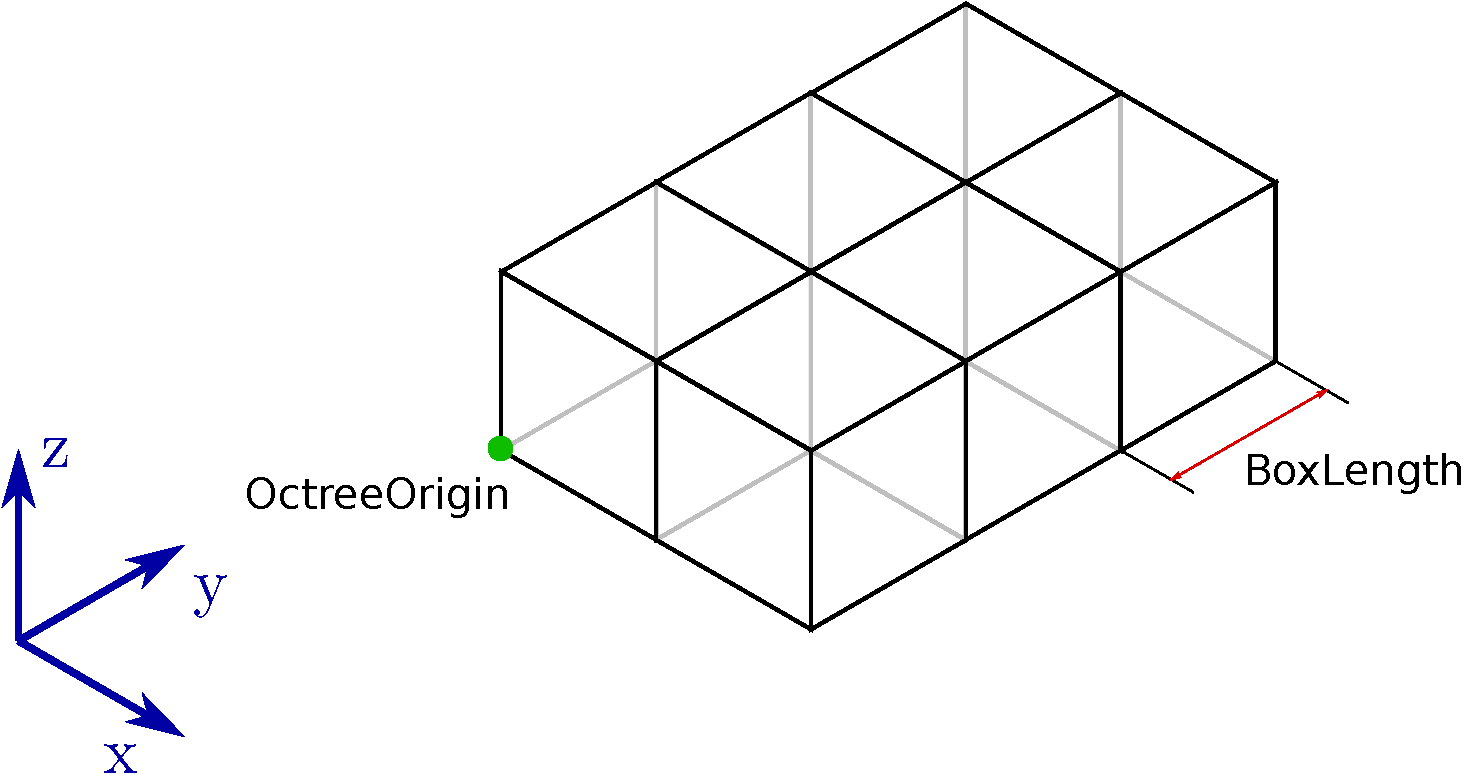
\includegraphics[width=.7\textwidth]{boxes}
\caption{System of cube boxes to compose the first level of the octree. 
In green is highlighted the origin of the octree, from which two rows of 
boxes in x, three in y and one in z starts, corresponding to \param{n_box} = (/2, 3, 1/). 
In red is highlighted the length of each cube side, \param{box_length}}
\label{fig:boxes1}
\end{figure}




\section{Time Stepping}
\label{sec:Time_Stepping}
The simulation is started from parameter \param{tstart} 
(unless restarting from a previous solution and not resetting time) 
and ends at \param{tend} after a certain number of timesteps. 
The user must provide the parameters \param{tstart}, \param{tend} 
and alternatively the number of timesteps (\param{timesteps}) between 
them or the size of the timesteps (\param{dt}). The non specified 
parameter is computed during the execution.

When specifying the number of timesteps, the interval between the 
starting time (or re-starting time) and the end time is divided in 
a number \param{timesteps} of equal intervals, and then \param{timesteps}+1 
steps are executed, counting also the starting one.

When specifying the timestep length \param{dt}, the smallest number of 
steps to get to \param{tend} is executed. If the time interval cannot be 
divided into an integer number of timesteps, all the timesteps will be 
executed anyway with a timestep length of \param{dt}, and the last timestep 
will be shorter to arrive precisely at \param{tend}. It must however be 
noted that DUST is not designed at the moment to handle variable timestep 
lengths, for this reason in few particular unsteady configurations, this 
shorter timestep could lead to small fluctuations of the loads just in the 
last timestep. To avoid this issue use a \param{dt} which lead to a precise 
number of timesteps or prescribe the number of timesteps instead of the 
timestep length (or discard the results of the last step). 

\section{Models Parameters Choice}
\label{sec:Solver_ParametersChoice}
In the previous section \ref{sec:Solver_InputFile} all the available 
parameters for the \DUST{} solver have been listed. While the brief 
description in most of the cases is enough to describe the simple 
functioning of the parameters, for some model parameters is necessary 
a more comprehensive discussion. 

\paragraph{Vortex Models Parameters}
%\textcolor{red}{Rewrite! or cancel it}

In \DUST{} all the description of both the surface elements and 
the wake relies (also) on vortex models. The vortex particles 
represent a small vortex unit, lifting lines are represented by 
a single vortex, panel wakes, vortex lattices and surface panels 
all have a uniform distribution of doublets, which is equivalent 
to a vortex ring along the sides of such panels. 

The velocity induced by vortexes decreases with a certain power 
of the distance from the vortex ($1/r$ in two dimensions, $1/r^2$ in three), 
which means that while at higher distances the induced velocity becomes 
small, for distances approaching zero the velocity becomes very high 
and eventually singular. This model is completely irrotational, with 
all the vorticity confined in a point/line, but is clearly not physical, 
and for this reason it is necessary to regularize the induced velocity 
in the proximity of the vortex. If in the case of the panels this can 
be seen merely as a regularization, in the case of the vortex particles 
the use of a regularized core is necessary to have a rotational volume 
for each particle which is able to represent the vorticity field generated 
by the wake. 

Starting precisely from this consideration, it is advisable to set the 
parameter \param{vortex_rad}, which is the radius of the Rosenhead 
regularized core employed for the vortex particles, to a value which
allow the generated particles to represent the whole generated vorticity 
field, by slightly overlapping one another. This can be done for example 
by setting \param{VotexRad} equal to the (average) length of the trailing 
edge element sides, where the particles are first generated and spaced.

Since the generation of the particles from the trailing edges sets somehow 
the spacing, and the resolution, of the vortical phenomena, the radius of 
the vortex model of the panels, \param{rankine_rad} should be chosen at least 
in the same order of magnitude of \param{vortex_rad}. The vortex 
regularization performed on the panels is the classical Rankine one. 
Since it is expected that the vortical phenomena on surfaces are more 
confined than in the wake the user might want to take a little smaller 
radius for the surface panels than the particles one, however remaining 
in the same order of magnitude. Too small radii might lead to not physical, 
too strong interactions with close particles or panels.

Eventually for the panels the parameter \param{cutoff_rad} sets a radius 
underneath which the interaction is set to zero, to avoid any kind of 
modelling when a point is essentially coinciding with the vortex. 
This parameter should be set \emph{much smaller} than \param{rankine_rad}. 


\section{Reference frames}
\label{sec:Solver_ReferenceFrames}

The reference frames are the basis for both the placement of the geometry 
components in the space and for the definition of their movement.  
Reference frames are handled by the solver, which reads them from 
a separate input file, indicated in the solver input file, file 
\ref{file:dust.in}. Before detailing the inputs for the reference 
frames file it is important to understand how reference frames work 
inside DUST. %(more details are presented in the Theory Manual).

Reference frames are defined hierarchically from a base reference frame. 
The base reference frame is called "0" and cannot be defined, 
is a standard right-nanded Cartesian reference frame and is defined 
inside DUST. Starting from the base reference frame all the necessary 
reference frames can be defined. 

It is important to stress that the base reference frame it is not 
defined upon any other implied reference frame and thus has no implied 
orientation with respect to anything else. Instead it is just the definition 
of the three axis x-y-z upon which all the other reference frames, geometrical 
components, parameters are defined. The user can give any meaning to the three 
axis, e.g. x horizontal towards rear, y horizontal towards right and z vertical 
upward, but also x front, y up and z right. The user must be then consistent 
with the inputs, both in terms of geometry and for example free stream velocity, 
but there is no implied orientation in the base reference.

All the following reference frames are defined upon another reference frame, 
called "parent" reference frames. Obviously the parent reference frame must 
always be defined, so that all the branches of the tree defined by the multiple 
reference frame can be traversed back to the base reference frame. The relative 
positioning of two reference frames with respect to the base one is depicted in 
figure \ref{fig:references1}. The use of multiple reference frames allows to 
position a geometrical entity, with its own local coordinates, in any position 
of the domain, and in any relative position with respect to the other components, 
in a logical way.  An example of references file, for static references is 
presented in file \ref{file:references_static.in}. 

\begin{figure}
\centering
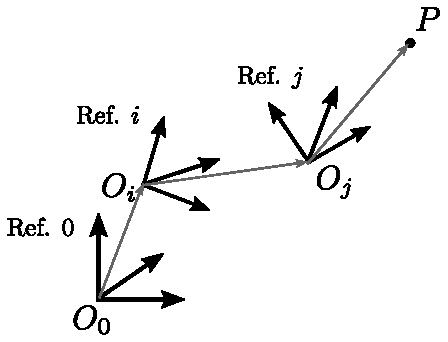
\includegraphics[width=.7\textwidth]{references1}
\caption{Positioning of relative reference frame}
\label{fig:references1}
\end{figure}

\begin{inputfile}[frame=single, caption={references\_static.in}, 
    label={file:references_static.in}]
!!!!!!!!!!!!!!!!!!!!!!!!!!!!!!!!!!!!!!!!!!!!!!!!!!!!!!!!!!!!!!!!!!!!!!!!!!!!!!!
reference_tag = root
parent_tag = 0
origin = (/0.0, 0.0, 0.0/)
orientation = (/1.0,0.0,0.0, 0.0,1.0,0.0, 0.0,0.0,1.0/)
multiple = F
moving = F

!!!!!!!!!!!!!!!!!!!!!!!!!!!!!!!!!!!!!!!!!!!!!!!!!!!!!!!!!!!!!!!!!!!!!!!!!!!!!!!
reference_tag = first
parent_tag = Root
origin = (/10.0, 2.0, 4.0/)
orientation = (/0.0,1.0,0.0, 0.0,0.0,1.0, 1.0,0.0,0.0/)
multiple = F
moving = F

!!!!!!!!!!!!!!!!!!!!!!!!!!!!!!!!!!!!!!!!!!!!!!!!!!!!!!!!!!!!!!!!!!!!!!!!!!!!!!!
reference_tag = second
parent_tag = Root
origin = (/0.0, 0.0, 0.0/)
orientation = (/0.999941,0.0,-0.010859, 0.0,1.0,0.0, +0.010859,0.0,0.999941/)
multiple = F
moving = F
\end{inputfile}
The details of the parameters are:
\begin{itemize}
\item \param{reference\_tag}: \textit{required:} yes. \textit{multiple:} yes. 
\textit{type:} string.

The tag is a unique identifier of the reference frame, it is a string and is 
referenced by the geometry component and other reference frames. All tags are 
valid except for "0" which is reserved by the base reference frame. 

The number of references tags declares the number of reference frames defined.

\item \param{parent\_tag}: \textit{required:} yes, in same number as \param{reference\_tag}. 
\textit{multiple:} yes. \textit{type:} string.

Declares the reference frame upon which the current reference frame is defined. 
The valid values are all the other reference frames defined in the input file 
(also later in the file) and "0". 

\item \param{origin}: \textit{required:} yes, in same number as \param{reference\_tag}. 
\textit{multiple:} yes. \textit{type:} real array of length 3.

origin of the current reference frame, in coordinates of the parent reference frame 
(not the global ones). 

\item \param{orientation}: \textit{required:} yes, in same number as \param{reference\_tag}. 
\textit{multiple:} yes. \textit{position:} must follow \param{origin} 
\textit{type:} real array of length 9.

orientation of the current reference frame with respect to the previous one. 
Considering a Fortran filling order (fastest cycling index is the row one), 
the 9 component vector forms a matrix with the vectors of the current base 
in the components of the parent base, by columns. In other words the first 
three coefficients represent the components of the x axis of the current frame 
in the parent frame, and so on for y and z axis. 

\item \param{multiple}: \textit{required:} yes, in same number as \param{reference\_tag}. 
\textit{multiple:} yes. \textit{type:} logical.
Is the reference frame multiple? 

\item \param{moving}: \textit{required:} yes, in same number as \param{reference\_tag}. 
\textit{multiple:} yes. \textit{type:} logical.
Is the reference frame moving with respect to the parent? 
\end{itemize}

\section{Moving reference frames}
Special input is required when a reference frame is moving or is multiple, 
in which case a special grouping keyword is required. 
As shown in file \ref{file:references_moving.in} if the parameter \param{moving} 
is set to true, it must be followed by the grouping parameter \param{motion} 
in which the definition of the motion is provided. 

All the motions in DUST are provided as a translation of a pole and a 
rotation around an axis passing from the pole, as depicted in figure 
\ref{fig:references2}. The motion of the pole can be defined in terms 
of position or velocity. Both can be described with some simple functions 
or from a time history from a data file.
In the same way the rotation around an axis can be defined in terms 
of angle or rotation rate, and with simple functions or data input.

The simple functions are either a constant value, or a sinusoidal function 
of time defined as
\begin{equation}
f(t) = A \sin{\omega t + \phi} + r 
\end{equation}
where $A$ is the amplitude, $\omega$ the pulsation, $\phi$ the phase and $r$ an offset. 

\begin{inputfile}[frame=single, caption={references\_moving.in}, 
    label={file:references_moving.in}]
!!!!!!!!!!!!!!!!!!!!!!!!!!!!!!!!!!!!!!!!!!!!!!!!!!!!!!!!!!!!!!!!!!!!!!!!!!!!!!!
reference_tag = moving
parent_tag = 0
origin = (/0.0, 1.0, 0.0/)
orientation = (/1.0,0.0,0.0, 0.0,1.0,0.0, 0.0,0.0,1.0/)
multiple = F
moving = T
motion = {
  pole = {
    input      = position                           
    input_type = simple_function
    function   = (/  0  ,  0  ,  0  /)
    !file       = xxx.dat
    amplitude  = 0.00
    vector     = (/ 0.0 , 0.0 , 0.0 /)
    omega      = (/ 0.0 , 0.0 , 0.0 /)
    phase      = (/ 0.0 , 0.0 , 0.0 /)
    offset     = (/ 0.0 , 0.0 , 0.0 /)
    !position_0 = ...
  }
  rotation   = {
    input      = position
    input_type = simple_function
    !file = ...
    function   =  1      
    Axis       = (/ 0.0 , 1.0 , 0.0 /)  
    amplitude  = 0.1    
    omega      = 1.2566  
    phase      = 0.0  
    offset     = 0.0  
    psi_0      = 0.0           
  }
}
\end{inputfile}

The details of the parameters inside the \param{motion} group are:
\begin{itemize}
\item \param{pole}: \textit{required:} yes. \textit{multiple:} 
not inside each \param{motion} group.

Grouping keyword containing the specification of the pole motion, 
the pole motion parameters are

	\begin{itemize}
	\item \param{input}: \textit{required:} yes. \textit{multiple:} 
    not inside each \param{pole} group. \textit{type:} string.
    
    In which way motion is imposed, can be \opt{position} or \opt{velocity}
    
    \item \param{input\_type}: \textit{required:} yes. \textit{multiple:} 
    not inside each \param{pole} group. \textit{type:} string.
    
    type of input, can be \opt{simple\_function} or \opt{from\_file}
    
    \item \param{function}: \textit{required:} yes if \param{input\_type} 
    is \opt{simple\_function}. \textit{multiple:} not inside each \param{pole} 
    group. \textit{type:} integer array of length 3.
    
    type of function to be imposed, at the moment \opt{0} is for a constant 
    function and \opt{1} is for a sinusoidal function. An array of three 
    components is expected, one for each direction of the pole motion.    

        \item \param{file}: \textit{required:} yes if \param{input\_type} 
        is \opt{from\_file}. \textit{multiple:} not inside each \param{pole} 
        group. \textit{type:} string.
        
        name of the file where the time history is of the motion 
        (position or velocity) is stored. The file is supposed to have 
        4 columns, the first containing a series of time values adequate 
        for the simulation time, and the following three the three components 
        of the pole motion. 
        
    \item \param{amplitude}: \textit{required:} no, used only if \param{input\_type}     
    is \opt{simple\_function}. \textit{multiple:} not inside each \param{pole} group. 
    \textit{default:} 1.0 \textit{type:} real.
    
    Collective amplitude of the motion, applied to all the three components of the motion    
    
     \item \param{vector}: \textit{required:} no, used only if \param{input\_type} 
     is \opt{simple\_function}. \textit{multiple:} not inside each \param{pole} group. 
     \textit{default:} (/1.0, 1.0, 1.0/) \textit{type:} real array of length 3.
    
    Relative amplitude of the motion for each component
    
    \item \param{omega}: \textit{required:} no, used only if \param{input\_type} 
    is \opt{simple\_function}. \textit{multiple:} not inside each \param{pole} group. 
    \textit{default:} (/1.0, 1.0, 1.0/) \textit{type:} real array of length 3
    
    Pulsation of each sinusoidal motion. Considered only if input is 
    \opt{simple\_function} and only for the components with sinusoidal functions.
    
    \item \param{phase}: \textit{required:} no, used only if \param{input\_type} 
    is \opt{simple\_function}. \textit{multiple:} not inside each \param{pole} group. 
    \textit{default:} (/0.0, 0.0, 0.0/) \textit{type:} real array of length 3.
    
    phase of each sinusoidal motion. Considered only if input is \opt{simple\_function} 
    and only for the components with sinusoidal functions.
    
    \item \param{offset}: \textit{required:} no, used only if \param{input\_type} 
    is \opt{simple\_function}. \textit{multiple:} not inside each \param{pole} group. 
    \textit{default:} (/0.0, 0.0, 0.0/) \textit{type:} real array of length 3.
    
    Constant offset (position/velocity) for each component of the pole motion
    
    \item \param{Position\_0}: \textit{required:} no, used only if \param{input\_type} 
    is \opt{simple\_function}. \textit{multiple:} not inside each \param{pole} group. 
    \textit{default:} (/0.0, 0.0, 0.0/) \textit{type:} real array of length 3
    
    Starting position of the pole in the three component, considered only if 
    \param{input} is \opt{velocity}
    
	\end{itemize}

\item \param{rotation}: \textit{required:} yes. \textit{multiple:} not inside each 
\param{motion} group.

Grouping keyword containing the specification of the rotation, which parameters are:

	\begin{itemize}
	\item \param{input}: \textit{required:} yes. \textit{multiple:} not inside each 
    \param{rotation} group. \textit{type:} string.
    
    In which way the rotation is imposed, can be \opt{position} for imposing an angle  
    or \opt{velocity} for imposing a rotation rate
    
    \item \param{input\_type}: \textit{required:} yes. \textit{multiple:} not inside 
    each \param{rotation} group. \textit{type:} string.
    
    type of input, can be \opt{simple\_function} or \opt{from\_file}
    
    \item \param{function}: \textit{required:} yes if \param{input\_type} is 
    \opt{simple\_function}. \textit{multiple:} not inside each \param{rotation} group. 
    \textit{type:} integer.
    
    type of function to be imposed, at the moment \opt{0} is for a constant function 
    and \opt{1} is for a sinusoidal function.
    
        \item \param{file}: \textit{required:} yes if \param{input\_type} is 
        \opt{from\_file}. \textit{multiple:} not inside each \param{rotation} group. 
        \textit{type:} string.
        
        name of the file where the time history is of the rotation 
        (angle or rotation rate) is stored. The file is supposed to have 2 columns, 
        the first containing a series of time values adequate for the simulation time, 
        and the following the rotation around the axis. 
        
    \item \param{Axis}: \textit{required:} yes. \textit{multiple:} not inside each 
    \param{rotation} group. \textit{type:} real array of length 3.
    
    orientation of the rotation axis, in the parent reference frame. The rotation 
    axis keeps a constant orientation in the parent reference frame and always passes 
    through the pole during its motion
    
    \item \param{amplitude}: \textit{required:} no, used only if \param{input\_type} 
    is \opt{simple\_function}. \textit{multiple:} not inside each \param{rotation} group. 
    \textit{default:} 1.0 \textit{type:} real.
    
    Collective amplitude of the rotation 
    
    \item \param{omega}: \textit{required:} no, used only if \param{input\_type} 
    is \opt{simple\_function}. \textit{multiple:} not inside each \param{rotation} group. 
    \textit{default:} 1.0 \textit{type:} real.
    
    Pulsation of the sinusoidal motion. Considered only if \param{input} is 
    \opt{simple\_function} and \param{input\_type} is a sinusoidal function.
    
        \item \param{phase}: \textit{required:} no, used only if 
        \param{input\_type} is \opt{simple\_function}. \textit{multiple:} not 
        inside each \param{rotation} group. \textit{default:} 0.0 \textit{type:} real.
    
    phase of the sinusoidal motion. Considered only if \param{input} is 
    \opt{simple\_function} and \param{input\_type} is a sinusoidal function.
    
    \item \param{offset}: \textit{required:} no, used only if \param{input\_type} 
    is \opt{simple\_function}. \textit{multiple:} not inside each \param{rotation} group. 
    \textit{default:} 0.0 \textit{type:} real.
    
    Constant offset of rotation or rotation rate
    
    \item \param{Psi\_0}: \textit{required:} no, used only if \param{input\_type} 
    is \opt{simple\_function}. \textit{multiple:} not inside each \param{rotation} group. 
    \textit{default:} 0.0 \textit{type:} real.
    
    Starting angle of the rotation, considered only if \param{input} is \opt{velocity}
    
	\end{itemize}

\end{itemize}

\begin{figure}
\centering
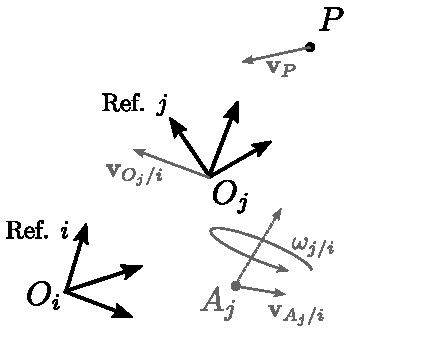
\includegraphics[width=.7\textwidth]{references2}
\caption{Velocity of relative reference frame}
\label{fig:references2}
\end{figure}

\section{Multiple reference frames}
To ease the setup of rotors in terms of reference frames and motions, 
a special set of instructions have been developed for the reference frames. 
Declaring a reference frame multiple, a single component is replicated n times 
in a special set of multiple, automatically generated reference frames. 
While there is possibility to expansion towards different types of multiple 
reference frames, at the moment multiplicity is employed only for rotors: an 
example input file with a reference frame for a rotor is given in file 
\ref{file:references_rotor.in}. 

\begin{inputfile}[frame=single, caption={references\_rotor.in}, label={file:references_rotor.in}]
!!!!!!!!!!!!!!!!!!!!!!!!!!!!!!!!!!!!!!!!!!!!!!!!!!!!!!!!!!!!!!!!!!!!!!!!!!!!!!!
reference_tag = Rotor01
parent_tag = Root
origin = (/0.0, 0.0, 0.0/)
orientation = (/1.0,0.0,0.0, 0.0,1.0,0.0, 0.0,0.0,1.0/)
moving = F
multiple = T
multiplicity = {
  mult_type = rotor
  n_blades = 4
  rot_axis = (/0.0, 0.0, 1.0/)
  rot_rate = 6.28318530717959 !2*pi, T=1
  psi_0 = 0.0
  hub_offset = 0.0

  n_dofs = 3
  dof = {
    hinge_type = Flap
    hinge_offset = (/ 0.0 , 0.032432 , 0.0 /)
    Collective  =  3.0     ! deg
    cyclic_ampl =  0.0     ! deg
    cyclic_phas =  0.0     ! deg
  }
  dof = {
    hinge_type = Lag
    hinge_offset = (/ 0.0 , 0.021622 , 0.0 /)
    Collective  = -10.0
    cyclic_ampl =  0.0
    cyclic_phas =  0.0
  }
  dof = {
    hinge_type = Pitch
    hinge_offset = (/ 0.0 , 0.086486 , 0.0 /)
    Collective  = 12.0
    cyclic_ampl =  0.0
    cyclic_phas =  0.0
  }

}


\end{inputfile}
Note that the rotor reference frame in file \ref{file:references_rotor.in} 
is set as not moving. This means that the starting reference frame is stationary 
(with respect to its parent) however all the other reference frames that are 
automatically generated move in order to represent the different movements of a rotor.

If in the reference frame specification the parameter \param{multiple} 
is set to true, it must be followed by a grouping keyword, \param{multiplicity}, 
which must contain the details of the multiplicity. The detailed parameters 
required in the multiplicity are:
\begin{itemize}
	\item \param{mult_type}: \textit{required:} yes. \textit{multiple:} 
    not inside each \param{multiplicity} group. \textit{type:} string.
    
	type of multiplicity. At the moment only \opt{rotor} is enabled.
    
    \item \param{N\_Blades}: \textit{required:} yes if \param{mult_type} 
    is \opt{rotor}. \textit{multiple:} not inside each \param{multiplicity} group. 
    \textit{type:} integer.
    
    Number of blades of the rotor. It is also the number of time the geometrical 
    component associated with the reference frame will be multiplied in the domain. 
    
    \item \param{Rot\_Axis}: \textit{required:} yes if \param{mult_type} is \opt{rotor}. 
    \textit{multiple:} not inside each \param{multiplicity} group. 
    \textit{type:} real array of length 3.
    
    Axis of rotation of the rotor, with respect to the current reference frame
    
    \item \param{Rot\_Rate}: \textit{required:} yes if \param{mult_type} is \opt{rotor}. 
    \textit{multiple:} not inside each \param{multiplicity} group. \textit{type:} real.
    
    rotation rate of the blades around the rotation axis. 
    The rotation of the rotor is kept constant.
    
    \item \param{Psi\_0}: \textit{required:} yes if \param{mult_type} is \opt{rotor}. 
    \textit{multiple:} not inside each \param{multiplicity} group. \textit{type:} real.
    
    Starting angle of the rotor at the beginning of the simulation
    
    \item \param{Hub\_Offset}: \textit{required:} yes if \param{mult_type} is \opt{rotor}. 
    \textit{multiple:} not inside each \param{multiplicity} group. \textit{type:} real. 
    
    offset from the rotation pole (the origin of the multiple reference frame) of the beginning of the chain of reference frames for each blade. It is constant and does not imply any secondary motion, can be used to represent the central part of the rotor axis assembly. 
    
    \item \param{N\_dofs}: \textit{required:} yes if \param{mult_type} is \opt{rotor}. 
    \textit{multiple:} not inside each \param{multiplicity} group. \textit{type:} integer.
    
    Number of additional degrees of freedom of each blade, generally representing 
    a movement around one of the blades hinges
    
    \item \param{dof}: \textit{required:} yes if \param{N\_dofs} is greater than zero. 
    \textit{multiple:} yes, in the number defined by \param{N\_dofs}. 
    
    Grouping keyword containing the details about geometry and movement of 
    one additional degree of freedom. The degrees of freedom are connected in 
    a chain according to the order in which are defined. A representation of 
    the chain of degrees of freedom is presented in figure \ref{fig:multiple_refs}.
    
    \begin{itemize}
    \item \param{hinge\_Type}: \textit{required:} yes. \textit{multiple:} 
    not inside each \param{dof} group. \textit{type:} string.
    
    type of hinge considered, affecting the axis of rotation of the hinge 
    movement with respect to the rotor axis, can be \opt{Flap},\opt{Lag}, or \opt{Pitch}.
    
    \item \param{hinge\_Offset}: \textit{required:} yes. \textit{multiple:} 
    not inside each \param{dof} group. \textit{type:} real array of length 3.
    
    offset of the hinge rotation axis with respect to the previous hinge or 
    the rotor hub (axis + hub offset).
    
    \item \param{Collective}: \textit{required:} yes. \textit{multiple:} not 
    inside each \param{dof} group. \textit{type:} real.
    
    Collective (constant during rotation) angle of rotation (in degrees) of 
    the degree of freedom.
    
    \item \param{Cyclic\_Ampl}: \textit{required:} yes. \textit{multiple:} 
    not inside each \param{dof} group. \textit{type:} real.
    
    Cyclic (sinusoidal during rotation) angle of rotation (in degrees) of 
    the degree of freedom.
    
    \item \param{Cyclic\_Phas}: \textit{required:} yes. \textit{multiple:} 
    not inside each \param{dof} group. \textit{type:} real.
    
    phase of the cyclic movement, in degrees, with respect to the rotor rotation. 
    
    \end{itemize}
\end{itemize}

\begin{figure}
\centering
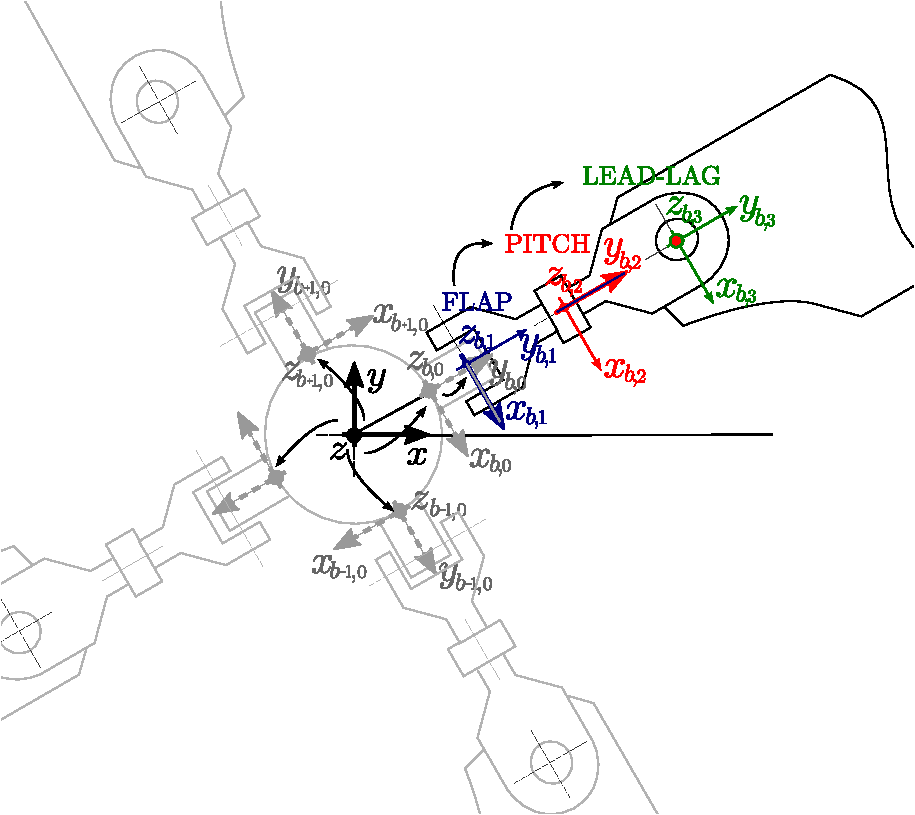
\includegraphics[width=.7\textwidth]{rotor_scheme}
\caption{multiple reference frames in a rotor}
\label{fig:multiple_refs}
\end{figure}

\section{Dimensional Units}
\label{sec:Dimensional_Units}

In the present section the dimensional units, normalization (or the lack of it) 
in \DUST{} will be discussed.

All the equations, models, inputs, outputs etc. in the code are \textbf{dimensional}. 
This does not mean that they are required to be in a specific dimensional unit, 
but only that \textbf{no sort of non-dimensionalization is performed in the code}. 
The user is fully resposible for the scaling (or not) of his inputs, and as a 
consequence of the outputs. 

More in detail the core of \DUST{} solves the potential equations, which are a 
simplified version of the incompressible Euler equations. Such equations do not 
depend on a scaling parameter (such as Mach or Reynolds for compressible Navier-Stokes) 
so their (scaled) results are independent on the scaling employed. Three possible 
approaches at the scaling of the variables and results are given in examples 
\ref{ex:pot-dim},\ref{ex:pot-nondim} and \ref{ex:pot-part}. 

\begin{example}[Potential case, fully dimensional]
\label{ex:pot-dim}
Consider a isolated wing with span $b = 20 m$ and chord $c = 2 m$ flying at 
$U = 60 m/s$ in air with density $\rho = 1.225 kg/m^3$. 

The user can take a completely dimensional approach and insert (or build) 
the geometry in the correct size in meters, and impose a free stream velocity 
and density corresponding to the real flight conditions. In this case the results, 
for example in terms of loads, will be in the same units set employed in the inputs, 
$L [N]$. To obtain the loads coefficient then the user must non-dimensionalize the 
results employing the appropriate reference quantities used in the computations:
\begin{equation*}
    C_L = \frac{L}{1/2 \rho U^2 b c} = \frac{L}{1/2 \cdot 1.225  \cdot 60^2 \cdot 20 \cdot 2}
\end{equation*}
\end{example}

\begin{example}[Potential case, fully scaled]
\label{ex:pot-nondim}
Starting from the conditions of example \ref{ex:pot-dim}, a user might want 
to re-scale all the quantities with respect to scaling units. For example, 
the geometry might be scaled by the span, giving $b' = b/b = 1$, $c'=c/b=0.1$ 
and introduced scaled from the mesh generator, scaled in the pre-processor or 
built parametrically already scaled. The velocity might be scaled on the free 
stream one, specifying directly $U'=U/U=1$, as well as the density $\rho' = \rho/\rho = 1$. 

With these parameters as input, the output would be scaled accordingly, 
leding for example to the scaled loads $L'$. These outputs, being scaled, 
are not numerically equal to the ones obtained in example \ref{ex:pot-dim}, 
however they can be on the one hand scaled back to the real ones employing 
the inverse scaling used for the inputs, or on the other hand if only the 
non-dimensional coefficients are sought they can be obtained using the scaled 
reference quantities:
\begin{equation*}
    C_L = \frac{L'}{1/2 \rho' U'^2 b' c'} = \frac{L'}{1/2 \cdot 1  \cdot 1^2 \cdot 1 \cdot 0.1}
\end{equation*}
When non-dimensionalized on the appropriate reference quantities the 
non-dimensional coefficients have always the same values.
\end{example}

\begin{example}[Potential case, partially scaled]
\label{ex:pot-part}
While in example \ref{ex:pot-nondim} all the quantities have been scaled 
with respect to some scaling quantity, the user can choose to use different 
quantities, or to scale only some of the quantities. For example, 
the user might want to keep the geometry from the CAD in meters, 
$b = 20 m$, $c = 2 m$ and scale the flight conditions for ease of use, 
$U'=U/U=1$, $\rho' = \rho/\rho = 1$. 

The results $L''$ are going to be again scaled, in a different way than 
in example \ref{ex:pot-nondim}, and the non-dimensional coefficient can 
be retrieved using the reference quantities employed in the computation:
\begin{equation*}
    C_L = \frac{L''}{1/2 \rho' U'^2 b c} = \frac{L''}{1/2 \cdot 1  \cdot 1^2 \cdot 20 \cdot 2}
\end{equation*}
\end{example}

It must however be stressed that when talking about scaling of the inputs 
and non-dimensionalization of the results, these operations are left to the 
user to be carried out independently before and after the execution of \DUST{}. 
To maintain complete usage flexibility, it is not possible to introduce any 
explicit scaling or non-dimensionalizing unit. 
When using certain features of the code (lifting lines, 
vorticity diffusion, separations etc.) the effects of viscosity 
and compressibility are simulated in different manners. 
To account for the right flow conditions it is necessary 
to specify the parameters governing the viscous and 
compressibility phenomena, i.e. the dynamic viscosity 
$\mu$ and the speed of sound $c$ in the input file. 
In continuity with the rest of the code, the dimensional physical 
properties of the flow must be provided, rather than the non dimensional 
numbers Reynolds and Mach. It is responsibility of the user to insert 
them correctly and eventually scale them to obtain similarity of Reynolds 
and Mach with respect to the target conditions. Examples on how to achieve 
that in different conditions are presented in example \ref{ex:rema-scaling}.

\begin{example}[Ways to determine physical properties]
\label{ex:rema-scaling}
Depending on the cases, the physical properties of the fluid to be given as input might be:
\begin{itemize}
    \item Already known and inserted as they are, if all the other reference 
    quantities have not be scaled
    \item Obtained from the original ones, keeping Reynolds and Mach number 
    equal, if some of the reference quantities were scaled:
    \begin{equation*}
        \frac{\rho U L}{\mu} = \frac{\rho' U' L'}{\mu'} \quad \rightarrow \quad \mu' = \mu \frac{\rho' U' L'}{\rho U L}
    \end{equation*}
    \begin{equation*}
        \frac{U}{c} = \frac{U'}{c'} \quad \rightarrow \quad c' = c \frac{U'}{U}
    \end{equation*}
    \item Obtained from the non-dimensional parameters, if those are known rather 
    than the properties of the fluid:
    \begin{equation*}
        Re = \frac{\rho' U' L'}{\mu'} \quad \rightarrow \quad \mu' = \frac{\rho' U' L'}{Re}
    \end{equation*}
    \begin{equation*}
        Ma = \frac{U'}{c'} \quad \rightarrow \quad c' = \frac{U'}{M}
    \end{equation*}
\end{itemize}
\end{example}

Finally, the reference pressure given as input is used as reference, 
free stream pressure, and does not affect the results except for a 
constant offset in the pressure field output. Loads are computed 
integrating on a closed surface and so are not affected by a constant 
offset on pressure. Knowing the reference pressure used as input, 
it is possible to retrieve the local coefficient of pressure:
\begin{equation*}
    C_p(\vec{x}) = \frac{P(\vec{x})-P_{ref}}{1/2 \rho U^2}
\end{equation*}
where $P(\vec{x})$ is the local pressure from the results, $P(\vec{x})$ 
is the reference pressure given as input and $\rho, U$ are the reference 
quantities employed during the simulation. 


\section{Debug Levels}
\label{sec:Solver_DebugLevels}

As discussed in section \ref{sec:Solver_InputFile} in the solver input 
file it is possible to set the parameter \param{debug\_level} which selects 
the verbosity of the output of the code. The level is selected choosing an 
integer number, and it is cumulative: selecting a certain value the user gets 
the additional output given at that value \emph{and} all the outputs at the lower levels. 
As a rule of thumb the debug levels up to 10 generate increasing levels of 
verbosity in the screen outputs, while increasing levels over 10 generate 
additional outputs saved in files, in the appropriate \param{basename\_debug} path. 
The current effects of the debug level are presented in table \ref{tab:debug_level}. 
Be aware that the debug file output is mainly targeted for development work, and its 
content is susceptible to sudden and undocumented changes. 

\begin{table}[]
\centering
\begin{tabular}{@{}rl@{}}
\toprule
Debug Level & Effects \\ \midrule
<0            & Almost no screen output, useful just for batch runs        \\
1             & Minimal screen output        \\
3             & Standard screen output information         \\ 
5             & Verbose screen output (fmm data etc.)\\
7             & Extra warnings and diagnostics, can lead to false negative warnings\\ 
8             & Extra verbose output (lifting lines data etc.)\\\midrule
15            & Output minimal geometry in ascii files \\
15            & Output extended geometry in ascii files \\
20            & Output the solution in ascii files \\
50            & Output the full linear system in ascii files\\
\bottomrule
\end{tabular}
\caption{\param{debug\_level} levels and their effects}
\label{tab:debug_level}
\end{table}

\section{Output Files}
\label{sec:Solver_Output_Files}

When running the solver, a certain number of hdf5 binary files are generated, 
in the location specified by \param{basename}. Two main type of files are generated:
\begin{itemize}
    \item \opt{basename}\_geo.h5: a file containing the geometry of the simulation, 
    which is similar to the input given to the solver, with some additions related 
    to the single simulation.
    \item \opt{basename}\_res\_XXXX.h5: a number of result files obtained during 
    the simulation, printed at the frequency specified in the input file. 
\end{itemize}

\chapter{DUST Postprocessor}
\label{ch:Post}

The DUST postprocessor is used to generate meaningful data from the binary 
results generated during the execution of the solver. While as discussed in 
\ref{sec:OutputFilesFormat} it is possible to look at the content of the hdf5 
results, these being based on the singularities intensities on the surface provide 
little insight on the solution of the solver. 

The postprocessor takes the specified results and use them to obtain a variety of 
different processed data, from visualizations to loads. 

The preprocessor is executed simply invoking the executable \texttt{dust\_post} 
in the desired folder. The input file containing all the required informations 
for the execution of the postprocessor must be passed as argument to the command call. 
If not provided explicitly the preprocessor automatically tries to read the default 
input file \texttt{dust\_post.in}.
\begin{command}[caption={Postprocessor command looking for input file 
  \texttt{input\_file\_name.in}}]
  dust_post input_file_name.in
\end{command}

\begin{command}[caption={Postprocessor command looking for 
default input file \texttt{dust\_post.in}}, label={command:dust_post_default}]
  dust_post
\end{command}

The different possible analysis that can be performed on the results are:
\begin{itemize}
\item \textbf{Integral loads}: history of loads acting on the geometry or parts 
      of the geometry
\item \textbf{Visualizations}: visualization of the surface solution 
      on the geometry and of the wake
\item \textbf{Probes}: Time history of certain variables probed in a 
      set of specified points
\item \textbf{Flow fields}: Visualization of the flow field in a structured 
      block domain
\item \textbf{Sectional loads}: distribution of the loads along a direction 
      on long aspect ratio components (i.e. wings or blades)
\end{itemize}


\section{input file}
\label{sec:Post_InputFile}

The input file of the postprocessor contains first all the information 
required for retrieving the correct results and to process the data 
(model parameters etc.) and then in separate sections all the analyses 
that are requested. An arbitrary number of analyses can be requested in 
a single input file, however it is also possible to group the analyses 
in different input files then invoked multiple times as different inputs 
for the postprocessor. 

The format is the same as all the other input files, as already specified 
in section\ref{sec:InputFilesFormat}.

A generic input file describing the main input is:

\begin{inputfile}[frame=single, caption={dust\_post.in}, label={file:dust_post.in}]
!--- Data Names ---
data_basename = ./Output/sim_results
basename =     ./Postpro/postpro_output

!--- Model Parameters (as in solver) ---
far_field_ratio_doublet = 10.0
far_field_ratio_source = 10.0
doublet_threshold = 1.0e-6
rankine_rad = 0.1
vortex_rad = 0.1
cutoff_rad = 0.001

analysis = {

type = viz  
name = vis01
start_res = 1
end_res   = 100 
step_res  = 1
format = vtk
wake = T
variable = vorticity 
}

analysis = {

type = integral_loads
name = load01
start_res = 1
end_res   = 100 
step_res  = 1
format = dat
average = F
component = all
reference_tag = RotorHub
}

\end{inputfile}

\begin{itemize}
\item \param{data\_basename}: \textit{required:} yes. \textit{multiple:} no. 

Base name (with path) of the data which must be analysed.

\item \param{basename}: \textit{required:} yes. \textit{multiple:} no. 

Base name (with path) of the postprocessing results

\item \param{far_field_ratio_doublet}: \textit{required:} no. 
\textit{multiple:} no. \textit{default:} 10

Ratio with respect to element length to set the thresholds for far field approximation. 
Same as in solver input file \ref{file:dust.in}.

\item \param{far_field_ratio_source}: \textit{required:} no. \textit{multiple:} no. 
\textit{default:} 10

As for \param{far_field_ratio_doublet} determines the threshold after which 
far field approximations are employed, just for sources. Same as in solver 
input file \ref{file:dust.in}.

\item \param{doublet_threshold}: \textit{required:} no. \textit{multiple:} no. 
\textit{default:} 1.0e-6

Parameter which sets the distance threshold under which the evaluation point, 
with respect to a panel, is considered inside the plane of the panel. 
Same as in solver input file \ref{file:dust.in}.

\item \param{rankine_rad}: \textit{required:} no. \textit{multiple:} no. 
\textit{default:} 0.1

Parameter which sets the radius under which the Rankine approximation of 
vortexes cores is employed. Used for aerodynamic elements and panels 
(i.e. everything except vortex particles). Same as in solver input file \ref{file:dust.in}.

\item \param{vortex_rad}: \textit{required:} no. \textit{multiple:} no. 
\textit{default:} 0.1

Parameter which sets the radius of the vortex particles. Same as in solver 
input file \ref{file:dust.in}.

\item \param{cutoff_rad}: \textit{required:} no. \textit{multiple:} no. 
\textit{default:} 0.001

Parameter which sets the radius under which the vortexes interaction is 
completely set to zero. Same as in solver input file \ref{file:dust.in}.

\item \param{analysis}: \textit{required:} at least one. \textit{multiple:} yes

Grouping keyword containing the information for a single postprocessing analysis.

\end{itemize}

The grouping keyword  \param{analysis} specifies a single analysis, 
and the parameters contained in the group depend on the type of the analysis. 
A series of  \param{analysis} groups can be contained in a single input file.

\subsection{Visualizations}

Visualizations are the main form of assessment of the results, 
they allow to see the movement of geometry and wake and the intensity 
of the solution on the surfaces and on the wake.

An example \param{analysis} group for a visualization is:

\begin{inputfile}[frame=single, caption={dust\_post.in for visualization}, 
  label={file:dust_post.in_viz}]
!--- Data Names ---
data_basename = ./Output/sim_results
basename =     ./Postpro/postpro_output

analysis = {

type = viz  
name = vis01
start_res = 1
end_res   = 100 
step_res  = 1
format = vtk
wake = T
average = F
variable = vorticity 
component = all

}
\end{inputfile}

\begin{itemize}
\item \param{type}: \textit{required:} one for each \param{analysis}. \textit{multiple:} no

type of the analysis, \opt{viz} for surface visualizations

\item \param{name}: \textit{required:} one for each \param{analysis}. \textit{multiple:} no

name of the analysis, will be appended as a suffix to \param{basename}

\item \param{start_res}: \textit{required:} one for each \param{analysis}. \textit{multiple:} no

First result in the time series of the solver results to analyse.

\item \param{end_res}: \textit{required:} one for each \param{analysis}. \textit{multiple:} no

Last result in the time series of the solver results to analyse.

\item \param{step_res}: \textit{required:} one for each \param{analysis}. \textit{multiple:} no

Stride to employ when loading the time series of the solver results. 

\item \param{format}: \textit{required:} one for each \param{analysis}. \textit{multiple:} no

format of the processed results, can be \opt{vtk} for vtk output or \opt{tecplot} 
for tecplot \opt{plt} files

\item \param{wake}: \textit{required:} no. \textit{multiple:} no. \textit{default:} True

Output the wake in the postprocessing.

\item \param{separate_wake}: \textit{required:} no. \textit{multiple:} no. 
\textit{default:} False

Since in vtk output is difficult to separate in the visualization process the 
different pieces of the solution, it is possible to output the wake in separate 
files with respect to the surface solution. It affects only the vtk output and 
only if \param{wake} is set to true.

\item \param{average}: \textit{required:} no. \textit{multiple:} no. \textit{default:} False

average the results in the given time span, and output just one averaged result. 
When used in visualizations, \param{wake} must be False.

\item \param{variable}: \textit{required:} at least one for each \param{analysis}. 
\textit{multiple:} yes.

variable to output in the processed result. More than one variable can be generated 
in the same analysis. At the moment \opt{vorticity}, \opt{pressure} and 
\opt{surface\_velocity} are implemented.

Note that that even if the keyword \opt{vorticity} is employed, the printed result 
is labelled \opt{singularity\_intensity} since it represent the intensity of the 
surface/point solution on the different elements. The keyword is likely to 
be changed also in the future releases.

\item \param{component}: \textit{required:} no. \textit{multiple:} yes. \textit{default:} all.

Geometrical component to include in the visualization. More component can be included. 
If not declared, or if declared \opt{all} all the components are loaded and processed. 
\end{itemize}

\subsection{Integral loads}

Integral loads allow to obtain the time history of the loads acting on one 
or more components, in one of the reference frames defined in section 
\ref{sec:Solver_ReferenceFrames}.

An example \param{analysis} group for integral loads is:

\begin{inputfile}[frame=single, caption={dust\_post.in for integral loads}, 
  label={file:dust_post.in_load}]
!--- Data Names ---
data_basename = ./Output/sim_results
basename =     ./Postpro/postpro_output

analysis = {

type = integral_loads
name = load01
start_res = 1
end_res   = 100 
step_res  = 1
format = dat
average = F
component = all
reference_tag = RotorHub

}
\end{inputfile}

\begin{itemize}
\item \param{type}: \textit{required:} one for each \param{analysis}. \textit{multiple:} no

type of the analysis, \opt{integral\_loads} for integral loads

\item \param{name}: \textit{required:} one for each \param{analysis}. \textit{multiple:} no

name of the analysis, will be appended as a suffix to \param{basename}

\item \param{start_res}: \textit{required:} one for each \param{analysis}. \textit{multiple:} no

First result in the time series of the solver results to analyse.

\item \param{end_res}: \textit{required:} one for each \param{analysis}. \textit{multiple:} no

Last result in the time series of the solver results to analyse.

\item \param{step_res}: \textit{required:} one for each \param{analysis}. \textit{multiple:} no

Stride to employ when loading the time series of the solver results. 

\item \param{format}: \textit{required:} one for each \param{analysis}. \textit{multiple:} no

format of the processed results, can be \opt{dat} for formatted ascii files output or 
\opt{tecplot} for tecplot plt files

\item \param{average}: \textit{required:} no. \textit{multiple:} no. \textit{default:} False

average the results in the given time span.

\item \param{component}: \textit{required:} no. \textit{multiple:} yes. \textit{default:} all.

Geometrical component to include in the loads computation. More component can be included. 
If not declared, or if declared \opt{all} all the components are loaded and processed. 

\item \param{Reference\_Tag}: \textit{required:} yes. \textit{multiple:} no.

The tag of the reference frame in which the loads should be referred to. 

\end{itemize}

\subsubsection{Output .dat file}
The output file containing integral loads measurements in \param{.dat} format has 
the following structure.
The first 4 lines of the file constitute the header of the file. The first three 
lines contains the number of the geometrical components \param{n\_comp} whose loads 
are integrated, the tag of reference system in which the components of the integral 
loads are expressed, the tags of the \param{n\_comp} components analyzed. As an example,
\begin{inputfile}
  1:  # Integral loads: N.components: 2
  2:  #                 Ref.sys     : Wing1_Reference
  3:  #                 Components  : Wing1 , Wing2
\end{inputfile}
The fourth line is the header of the following lines, containing the time, 
the three components of force and moment loads, the 9 elements of the (unrolled) 
rotation matrix and the 3 global coordinates of the origin of the local reference 
system, required to compute the components of the loads in the global reference 
frame, given those in the local reference frame.
\begin{inputfile}
  4:  #  t , Fx , Fy , Fz , Mx , My , Mz , ref_mat(9) , ref_off(3) 
\end{inputfile}
The last lines of the file contain the actual data. As an example, for a 
100-timestep analysis with the local reference frame \param{Wing1\_Reference} 
aligned with the global reference frame (the rotation matrix is equal to the identity) 
and the origin in $(0.0,-1.0,0.0)$, these lines read
\begin{inputfile}
  5: 0.000000E+000  0.260753E+001  0.000000E+000  0.115993E+003
     0.150792E+003 -0.434173E+001 -0.338980E+001  0.100000E+001
     0.000000E+000  0.000000E+000  0.000000E+000  0.100000E+001
     0.000000E+000  0.000000E+000  0.000000E+000  0.100000E+001
     0.000000E+000 -0.100000E+001  0.000000E+000
...:
104: 0.858240E-002  0.545038E+001  0.000000E+000  0.830829E+002
     0.108007E+003 -0.312156E+001 -0.708549E+001  0.100000E+001
     0.000000E+000  0.000000E+000  0.000000E+000  0.100000E+001
     0.000000E+000  0.000000E+000  0.000000E+000  0.100000E+001
     0.000000E+000 -0.100000E+001  0.000000E+000
\end{inputfile}

\subsection{Hinge Loads}

Hinge loads allows to obtain the time history of the load acting to one control 
surface along the hinge axis reference frame as defined in figure~\ref{fig:hingeref}. 

An example \param{analysis} group for hinge loads is:

\begin{inputfile}
analysis = {
  type = hinge_loads
  name = hm

  start_res = 1
  end_res = 20
  step_res = 1

  format = dat
  average = F
  component = Wing
  hinge_tag = Aileron
}
\end{inputfile}

\begin{itemize}
\item \param{type}: \textit{required:} one for each \param{analysis}. \textit{multiple:} no

type of the analysis, \opt{hinge\_loads} for hinge loads

\item \param{name}: \textit{required:} one for each \param{analysis}. \textit{multiple:} no

name of the analysis, will be appended as a suffix to \param{basename}

\item \param{start_res}: \textit{required:} one for each \param{analysis}. \textit{multiple:} no

First result in the time series of the solver results to analyse.

\item \param{end_res}: \textit{required:} one for each \param{analysis}. \textit{multiple:} no

Last result in the time series of the solver results to analyse.

\item \param{step_res}: \textit{required:} one for each \param{analysis}. \textit{multiple:} no

Stride to employ when loading the time series of the solver results. 

\item \param{format}: \textit{required:} one for each \param{analysis}. \textit{multiple:} no

format of the processed results, can be \opt{dat} for formatted ascii files output or 
\opt{tecplot} for tecplot \opt{plt} files

\item \param{average}: \textit{required:} no. \textit{multiple:} no. \textit{default:} False

average the results in the given time span.

\item \param{component}: \textit{required:} no. \textit{multiple:} yes. \textit{default:} all.

Geometrical component to include in the loads computation. More component can be included. 
If not declared, or if declared \opt{all} all the components are loaded and processed. 

\item \param{hinge_tag}: \textit{required:} yes. \textit{multiple:} no.

The tag of the control surface of the component in which the loads should be referred to. 

\end{itemize}

\subsubsection{Output .dat file}
The output file containing hinge loads measurements in \param{.dat} 
format has the following structure.
The first 4 lines of the file constitute the header of the file. 
The first three lines contains the number of the geometrical components 
\param{n\_comp} whose loads are integrated, the tag of reference system 
in which the components of the integral loads are expressed, the tags of 
the \param{n\_comp} components analyzed. As an example,
\begin{inputfile}
 1: # hinge Moment: 
 2: #               Components  : Wing
 3: #                    hinge  : Aileron
\end{inputfile}
The fourth line is the header of the following lines, containing the time, 
the three components of force and moment loads, the 9 elements of the (unrolled) 
rotation matrix and the 3 global coordinates of the origin of the hinge reference 
system, required to compute the components of the loads in the global reference 
frame, given those in the hinge axis reference frame. The hinge moment is located 
always under the column \opt{Mh}. 
\begin{inputfile}
 4: #  t , Fv , Fh , Fn , Mv , Mh , Mn , axis_mat(9) , node_hinge(3) 
\end{inputfile}
The last lines of the file contain the actual data. As an example, 
for a 20-timestep analysis with the hinge  reference frame \param{Wing1\_Aileron} 
aligned with the global reference frame (the rotation matrix is equal to the identity)
and the origin of the hinge is $(0.25,-0.1,0.0)$, these lines read
\begin{inputfile}
  5: 0.000000E+000    0.212095E+004    -0.34102E-015  0.11784E+005  
     0.295794E+006    -0.28342E+004    -0.53235E+005  0.10000E+001  
     0.000000E+000    0.000000E+000    0.000000E+000  0.10000E+001  
     0.000000E+000    0.000000E+000    0.000000E+000  0.10000E+001  
     0.250000E+000    -0.10000E+000    0.000000E+000
  
...:
  25: 0.190000E+000  0.121453E+003 -0.75517E-017  0.643457E+003  
      0.161506E+005  -0.81645E+002 -0.30484E+004  0.100000E+001  
      0.000000E+000  0.000000E+000  0.00000E+000  0.100000E+001  
      0.000000E+000  0.000000E+000  0.00000E+000  0.100000E+001  
      0.25000E+000   -0.10000E+000  0.00000E+000
\end{inputfile}



\subsection{Probes}

Probes allow to obtain a time history of some variables in some points by 
sampling the solution at such points. 

An example \param{analysis} group for probes is:

\begin{inputfile}[frame=single, caption={dust\_post.in for probes}, 
  label={file:dust_post.in_probes}]
!--- Data Names ---
data_basename = ./Output/sim_results
basename =     ./Postpro/postpro_output

analysis = {

type = probes
name = prb01
start_res = 1
end_res   = 100 
step_res  = 1
format = dat

variable = Velocity

input_type = point_list
point = (/0.0, 1.0, 2.0/)
point = (/1.0, 0.0, -2.0/)

!input_type = from_file
!file = point_list.dat

}
\end{inputfile}

\begin{itemize}
\item \param{type}: \textit{required:} one for each \param{analysis}. 
\textit{multiple:} no

type of the analysis, \opt{probes} for probes

\item \param{name}: \textit{required:} one for each \param{analysis}. 
\textit{multiple:} no

name of the analysis, will be appended as a suffix to \param{basename}

\item \param{start_res}: \textit{required:} one for each \param{analysis}. 
\textit{multiple:} no

First result in the time series of the solver results to analyse.

\item \param{end_res}: \textit{required:} one for each \param{analysis}. 
\textit{multiple:} no

Last result in the time series of the solver results to analyse.

\item \param{step_res}: \textit{required:} one for each \param{analysis}. 
\textit{multiple:} no

Stride to employ when loading the time series of the solver results. 

\item \param{format}: \textit{required:} one for each \param{analysis}. 
\textit{multiple:} no

format of the processed results, can be \opt{dat} for formatted ascii files 
output or \opt{tecplot} for tecplot \opt{plt} files

\item \param{variable}: \textit{required:} at least one for each \param{analysis}. 
\textit{multiple:} yes.

variable to output in the processed result. More than one variable can be generated in the same analysis. 
At the moment \opt{Velocity}, \opt{Pressure} and \opt{cp} are implemented.

\item \param{input_type}: \textit{required:} one for each \param{analysis}. \textit{multiple:} no

The way the probing points are specified, \opt{point\_list} for a series of 
points specified directly in the input file, \opt{from\_file} to load the list 
of points from a formatted ascii file.

\item \param{point}: \textit{required:} at least one if \param{input_type} is \opt{point\_list} 
\textit{multiple:} yes.

Position of the probing point.

\item \param{file}: \textit{required:} yes if \param{input_type} is \opt{from\_file} \textit{multiple:} no.

Location and name of the file containing the list of probing points.

\end{itemize}

\subsubsection{Output .dat file}

The output file containing point probe measurements in \param{.dat} format has 
the following structure. The first line is a header containing the number of probes
\begin{inputfile}[frame=single]
 1:  # N. of point probes:           2
\end{inputfile}
and the following 3 lines contains the 3 global coordinates of the point probes. 
As an example, if the \param{n\_probes} = 2 probes have global cartesian coordinates 
$(0.0,1.0,2.0)$ and $(1.0,0.0,-2.0)$, these lines read
\begin{inputfile}[frame=single]
 2:  0.000000E+000  0.100000E+001
 3:  0.100000E+001  0.000000E+000
 4:  0.200000E+001 -0.200000E+001
\end{inputfile}
The fifth line is a header line, containing the description of the next lines. 
The first field is the time,
\begin{inputfile}[frame=single]
 5:  #    t     2(   ux  uy  uz )
\end{inputfile}
while \param{n\_probes} $\times$ 3 columns follow, containing the global 
components of the velocity vectors, measured by the point probes. 
The following lines contains the fields described for each time step 
required for the analysis. As an example, for a 100-timestep analysis 
these lines read
\begin{inputfile}[frame=single]
  6: 0.000000E+000  0.465000E+002  -0.899269E-004  -0.469068E-004  0.465000E+002
     0.633261E-004 -0.980265E-004   
...:
105: 0.858240E-002  0.465003E+002  -0.238562E-002  -0.119496E-002  0.465023E+002
     0.216758E-002 -0.357483E-002
\end{inputfile}

\subsection{Flow Field}

Flow fields allow to probe systematically the domain obtaining the solution 
probed in a structured series of points in 1-2 or 3 dimensions, allowing the 
visualization of the flow field induced by the solution of the singular elements.

An example \param{analysis} group for flow fields is:

\begin{inputfile}[frame=single, caption={dust\_post.in for flow fields}, 
  label={file:dust_post.in_flow_fields}]
!--- Data Names ---
data_basename = ./Output/sim_results
basename =     ./Postpro/postpro_output

analysis = {

type = flow_field
name = ff01
start_res = 1
end_res   = 100 
step_res  = 1
format = vtk
average = F

variable = Velocity

n_xyz = (/ 10, 10, 1/)
min_xyz = (/ -2.0, -2.0, 1.0 /)
max_xyz = (/ 2.0, 2.0, 1.0 /)
}
\end{inputfile}

\begin{itemize}
\item \param{type}: \textit{required:} one for each \param{analysis}. \textit{multiple:} no

type of the analysis, \opt{flow\_field} for flow fields

\item \param{name}: \textit{required:} one for each \param{analysis}. \textit{multiple:} no

name of the analysis, will be appended as a suffix to \param{basename}

\item \param{start_res}: \textit{required:} one for each \param{analysis}. \textit{multiple:} no

First result in the time series of the solver results to analyse.

\item \param{end_res}: \textit{required:} one for each \param{analysis}. \textit{multiple:} no

Last result in the time series of the solver results to analyse.

\item \param{step_res}: \textit{required:} one for each \param{analysis}. \textit{multiple:} no

Stride to employ when loading the time series of the solver results. 

\item \param{format}: \textit{required:} one for each \param{analysis}. \textit{multiple:} no

format of the processed results, can be \opt{vtk} for binary vtk files output 
or \opt{tecplot} for tecplot plt files

\item \param{average}: \textit{required:} no. \textit{multiple:} no. \textit{default:} False

average the results in the given time span, only one averaged result will be printed. 

\item \param{variable}: \textit{required:} at least one for each \param{analysis}. 
\textit{multiple:} yes.

variable to output in the processed result. More than one variable can be generated in the same analysis. 
At the moment \opt{Velocity}, \opt{Pressure} and \opt{cp} are implemented.

\item \param{n_xyz}: \textit{required:} one for each \param{analysis}. \textit{multiple:} no.

Number of points in each direction of the sampling box. To have a 2D plane or a 1D 
line insert 1 point as number of points in the relevant direction

\item \param{min_xyz}: \textit{required:} one for each \param{analysis}. 
\textit{multiple:} no.

Minimum of the coordinates of the box containing the structured sampling points.

\item \param{max_xyz}: \textit{required:} one for each \param{analysis}. 
\textit{multiple:} no.

Maximum of the coordinates of the box containing the structured sampling points.

\end{itemize}

\subsection{Sectional loads}

Sectional loads allow to obtain the distribution of the forces along one 
direction of a slender body, e.g. a wing or a blade. 

The way the sectional loads are retrieved is different when employing a 
parametrically generated element or a generic element 
(i.e. an unstructured mesh generated from a mesh generator). 

In the first case is sufficient to provide the reference line for the 
moments calculation, and the subdivision is already implied in the structure 
of the parametric element. 

An example \param{analysis} group for sectional loads on parametric components:

\begin{inputfile}[frame=single, caption={dust\_post.in for sectional load 
  on parametric components}, label={file:dust_post.in_sectional_param}]
!--- Data Names ---
data_basename = ./Output/sim_results
basename =     ./Postpro/postpro_output

analysis = {

type = sectional_loads
name = sl01
start_res = 1
end_res   = 100 
step_res  = 1
format = dat
average = F

component = wing

axis_nod = (/ 0.0, 0.0, 0.0 /)
axis_dir = (/ 0.0, 0.1, 0.0 /)

lifting_line_data = F
vortex_lattice_data = F
}
\end{inputfile}

\begin{itemize}
\item \param{type}: \textit{required:} one for each \param{analysis}. \textit{multiple:} no

type of the analysis, \opt{sectional\_loads} for sectional loads

\item \param{name}: \textit{required:} one for each \param{analysis}. \textit{multiple:} no

name of the analysis, will be appended as a suffix to \param{basename}

\item \param{start_res}: \textit{required:} one for each \param{analysis}. 
\textit{multiple:} no

First result in the time series of the solver results to analyse.

\item \param{end_res}: \textit{required:} one for each \param{analysis}. 
\textit{multiple:} no

Last result in the time series of the solver results to analyse.

\item \param{step_res}: \textit{required:} one for each \param{analysis}. 
\textit{multiple:} no

Stride to employ when loading the time series of the solver results. 

\item \param{format}: \textit{required:} one for each \param{analysis}. 
\textit{multiple:} no

format of the processed results, can be \opt{dat} for formatted ascii files 
output or \opt{tecplot} for tecplot plt files

\item \param{average}: \textit{required:} no. \textit{multiple:} no. 
\textit{default:} False

average the results in the given time span.

\item \param{component}: \textit{required:} one for each \param{analysis}. 
\textit{multiple:} no.

component (parametrically generated) to analyse. Only one component can be 
enabled for each analysis. 

\item \param{axis_nod}: \textit{required:} one for each \param{analysis}. 
\textit{multiple:} no.

Coordinates of the node from which to start the line around which to calculate 
the distribution of moment along the span.

\item \param{axis_dir}: \textit{required:} one for each \param{analysis}. 
\textit{multiple:} no.

Direction of the line (starting from \param{axis_nod}) around which to calculate 
the distribution of moment along the span.

\item \param{lifting_line_data}: \textit{required:} no. \textit{multiple:} no. 
\textit{Default:} False

\item \param{vortex_lattice_data}: \textit{required:} no. \textit{multiple:} no. 
\textit{Default:} False

Output additional informations regarding span distribution of several quantities 
of interest for the lifting lines. It works only for parametric elements which 
are lifting lines.

\end{itemize}

On generic components it is necessary to define an ordered slender box with 
orientation to prescribe the interpolation along a series of sections of the 
surface data of the components to obtain the distribution of loads along the 
prescribed direction.

An example \param{analysis} group for sectional loads on generic components:

\begin{inputfile}[frame=single, caption={dust\_post.in for sectional load on 
  generic components}, label={file:dust_post.in_sectional_param}]
!--- Data Names ---
data_basename = ./Output/sim_results
basename =     ./Postpro/postpro_output

analysis = {

type = sectional_loads
name = sl01
start_res = 1
end_res   = 100 
step_res  = 1
format = dat
average = F

component = wing

box_sect = {
 ref_node = (/ -0.5 ,-0.5 , -0.3 /)
 face_vec = (/ 1.0 , 0.0 , 0.0 /)
 face_bas = (/ 2.0 , 1.0 /) 
 face_hei = (/ 1.0 , 1.0 /)
 span_vec = (/ 0.0 , 1.0 , 0.0 /)
 span_len = 3.0
 num_sect = 10
 reshape_box = T 
} 


}
\end{inputfile}

\begin{itemize}
\item \param{type}: \textit{required:} one for each \param{analysis}. \textit{multiple:} no

type of the analysis, \opt{sectional\_loads} for sectional loads

\item \param{name}: \textit{required:} one for each \param{analysis}. \textit{multiple:} no

name of the analysis, will be appended as a suffix to \param{basename}

\item \param{start_res}: \textit{required:} one for each \param{analysis}. 
\textit{multiple:} no

First result in the time series of the solver results to analyse.

\item \param{end_res}: \textit{required:} one for each \param{analysis}. 
\textit{multiple:} no

Last result in the time series of the solver results to analyse.

\item \param{step_res}: \textit{required:} one for each \param{analysis}. 
\textit{multiple:} no

Stride to employ when loading the time series of the solver results. 

\item \param{format}: \textit{required:} one for each \param{analysis}. 
\textit{multiple:} no

format of the processed results, can be \opt{dat} for formatted ascii files 
output or \opt{tecplot} for tecplot plt files

\item \param{average}: \textit{required:} no. \textit{multiple:} no. 
\textit{default:} False

average the results in the given time span.

\item \param{component}: \textit{required:} one for each \param{analysis}. 
\textit{multiple:} no.

component to analyse. Only one component can be enabled for each analysis. 

\item \param{box_sect}: \textit{required:} one for each \param{analysis} 
if component not parametrically generated. \textit{multiple:} no.

Grouping keyword containing the information about the box generated to 
interpolate the sectional loads

\item \param{ref_node}: \textit{required:} one for each \param{box_sect}. 
\textit{multiple:} no.

Coordinates of the point from which to build the bounding box for the sectional loads.

\item \param{face_vec}: \textit{required:} one for each \param{box_sect}. 
\textit{multiple:} no.

Direction of the base faces of the bounding box (roughly the chord direction). 
The bounding box is extruded between the two faces. 

\item \param{face_bas}: \textit{required:} one for each \param{box_sect}. 
\textit{multiple:} no.

Lenght of the base faces in the \param{face_vec} direction. It must have 
two components, one for the first beginning face, one for the last end face. 

\item \param{face_hei}: \textit{required:} one for each \param{box_sect}. 
\textit{multiple:} no.

Height of the base faces, normal to the \param{face_vec} direction. It must 
have two components, one for the first beginning face, one for the last end face. 

\item \param{span_vec}: \textit{required:} one for each \param{box_sect}. 
\textit{multiple:} no.

Direction of the span for the sectional loads, indicates the direction between 
the beginning and end faces of the bounding box.

\item \param{span_len}: \textit{required:} one for each \param{box_sect}. 
\textit{multiple:} no.

Length of the span for the sectional loads, indicates the distance between 
the beginning and end faces of the bounding box.

\item \param{num_sect}: \textit{required:} one for each \param{box_sect}. 
\textit{multiple:} no.

Number of sections, i.e. subdivisions in the span direction of the box. 
The subdivision must be coarse enough to avoid having one single surface 
panel appearing in three different sections. This means that for an equally 
spaced mesh and a tightly fitted box that there should be a number of 
sections lower or equal to the number of surface elements in the span 
direction. 

\item \param{reshape_box}: \textit{required:} one for each \param{box_sect}. 
\textit{multiple:} no.

Enables the possibility to reshape a too loose sections box to closely 
fit the component. Automatically reduces the size of the span to fit the 
component, keeping the same number of subdivision (thus generating a 
finer subdivision than requested)

\end{itemize}

\subsubsection{Output .dat file}

The output file containing sectional loads in \param{.dat} format has 
the following structure. The first line is a header specifying the 
structural component analyzed and the force/moment component collected 
in the file. As an example,
\begin{inputfile}[frame=single]
 1: # Sectional load Fz of component: Wing1
\end{inputfile}
The second line contains the number of sections \param{n\_sec} in which the 
structural component is divided and the number of time steps \param{n\_time}
of the analysis. As an example, the output file for a 10-section blade reads
\begin{inputfile}[frame=single]
 2: # n_sec : 10 ; n_time : 100. Next lines: y_cen , y_span, chord
\end{inputfile}
The second line also introduce the content of lines 3, 4 and 5. Line 3 contains 
the spanwise coordinate \param{y\_cen} of the centre of the sections, 
line 4 contains the spanwise dimension \param{y\_span} of the section, and 
line 5 contains the  chord dimension \param{chord} of the section. As an 
example, if the the blade length is 0.6 and it is divided in 10 uniform sections with chord 0.05, 
the output file reads
\begin{inputfile}[frame=single]
 3:  0.30000E-001  0.90000E-001  0.15000E+000  0.21000E+000 ...
 4:  0.60000E-001  0.60000E-001  0.60000E-001  0.60000E-001 ...
 5:  0.50000E-001  0.50000E-001  0.50000E-001  0.50000E-001 ...
\end{inputfile}
The sixth line is another header file containing the fields and their 
dimension collected in the next \param{n\_time} lines.
\begin{inputfile}[frame=single]
 6: # t , sec(n_sec) , ref_mat(9) , ref_off(3) 
\end{inputfile}
The first field is the time. The sectional loads of the \param{n\_sec} 
sections follow. The last 12 lines contains the (first-column) unrolled 
3x3 rotation matrix the global components of the origin of the local 
reference frame, required to obtain the components of the loads in the 
global reference frame from those expressed in the local reference frame,
\begin{equation}
   \underline{f}^G = \underline{\underline{R}} \, \underline{f}^L \ .
\end{equation}
As an example, the lines collecting the fields described above of the 
first and the last of the 100 timesteps of the analysis reads
\begin{inputfile}[frame=single]
  7: 0.000000E+000  0.966615E+002  0.966615E+002  0.966615E+002  0.966615E+002
     0.966615E+002  0.966615E+002  0.966615E+002  0.966615E+002  0.966615E+002
     0.966615E+002  0.100000E+001  0.000000E+000  0.000000E+000  0.000000E+000
     0.100000E+001  0.000000E+000  0.000000E+000  0.000000E+000  0.100000E+001
     0.000000E+000 -0.100000E+001  0.000000E+000
...:
105: 0.858240E-002  0.571236E+002  0.701379E+002  0.755018E+002  0.780314E+002
     0.790800E+002  0.790800E+002  0.780314E+002  0.755017E+002  0.701378E+002
     0.571235E+002  0.100000E+001  0.000000E+000  0.000000E+000  0.000000E+000
     0.100000E+001  0.000000E+000  0.000000E+000  0.000000E+000  0.100000E+001
     0.000000E+000 -0.100000E+001  0.000000E+000
\end{inputfile}
The geometrical component of the example is attached to a steady 
reference frame, whose origin has global components $( 0.0, -1.0, 0.0 )$ 
and whose axes are aligned with those of the global reference frame, so 
that the rotation matrix $\underline{\underline{R}}$ is equal to the 
identity matrix.

The extra files produced if \param{lifting_line_data}  
or if \param{vortex_lattice_data} are set to \param{T} 
do not contain the 12 columns of the rotation matrix and 
the global components of the origin of the local reference frame.

The files generated by sectional loads contain, as sectional quantity:
\begin{itemize}
    \item \texttt{Fx}: force acting on the section, \texttt{x} direction 
    of the component local reference frame
    \item \texttt{Fy}: force acting on the section, \texttt{y} direction 
    of the component local reference frame
    \item \texttt{Fz}: force acting on the section, \texttt{z} direction 
    of the component local reference frame
    \item \texttt{Mo}: moment acting on the section, with respect to the 
    axis specified in the definition of the sectional load with \param{axis_nod} 
    and \param{axis_dir}
\end{itemize}
additionally, when \param{lifting_line_data} or \param{vortex_lattice_data} 
are set to \param{T} the following quantities are printed:
\begin{itemize}
    \item \texttt{Cl}: two dimensional lift coefficient of the section, 
    as retrieved from the lookup tables
    \item \texttt{Cd}: two dimensional drag coefficient of the section, 
    as retrieved from the lookup tables
    \item \texttt{Cm}: two dimensional moment coefficient of the section, 
    as retrieved from the lookup tables
    \item \texttt{vel\_2d}: magnitude of the projection of the relative 
    velocity (as the sum of the free stream velocity, the opposite of 
    the body velocity and the influence of all the singularities, 
    $\mathbf{v}_{rel} = \mathbf{v}_\infty - \mathbf{v}_b + 
    \mathbf{v}_{ind} = \mathbf{v}_{rel,free} + \mathbf{v}_{ind}$) 
    in the plane identified by the normal and tangential unit vectors 
    $\mathbf{\hat{n}}$, $\mathbf{\hat{t}}$, as represented in figure \ref{fig:ll_output},
    $v_{2d} = | \mathbf{v}_{rel} \cdot \mathbf{\hat{b}}|$.
    \item \texttt{vel\_outplane}: magnitude of the out-of-plane velocity, 
    $\mathbf{v}_{rel} \cdot \mathbf{\hat{b}}$, where 
    $\mathbf{\hat{b}} = \mathbf{\hat{n}} \times \mathbf{\hat{t}}$ 
    is the unit vector ``in the crossflow direction''
    \item \texttt{alpha}: angle of attack of the in plane relative 
    velocity at the control point, corrected with the 2D influence 
    needed by Piszkin and Lewinski formulation of LL elements, 
    in order to get the right angle of attack to be used in the 
    aerodynamic tables
    \item \texttt{vel\_2d\_isolated}: same as \texttt{vel\_2d} but 
    for the relative free stream velocity $\mathbf{v}_{rel,free}$ only,
    being the influence of the body and wake singularities neglected;
    \item \texttt{vel\_outplane\_isolated}: same as \texttt{vel\_outplane} 
    but for the relative free stream velocity $\mathbf{v}_{rel,free}$ only, 
    being the influence of the body and wake singularities neglected;
    \item \texttt{alpha\_isolated}: angle of attack of the in plane relative 
    free stream velocity at the control point, equal to 
    $\alpha_{is} = \text{atan2}( \mathbf{v}_{rel,free} \cdot \mathbf{\hat{n}}, 
    \ \mathbf{v}_{rel,free} \cdot \mathbf{\hat{t}})$.
\end{itemize}
% While the above quantities are computed taking into account the 
%influence from all the components and wakes, \texttt{alpha}, 
%\texttt{vel\_2d} and \texttt{vel\_outplane} are also printed in 
%their corresponding \texttt{isolated} version, where the quantities 
% are computed taking into account only the free stream velocity and 
%the possible movement of the component, but neglecting the influence 
%from all the other components and wakes. 

\begin{figure}[h]
\centering
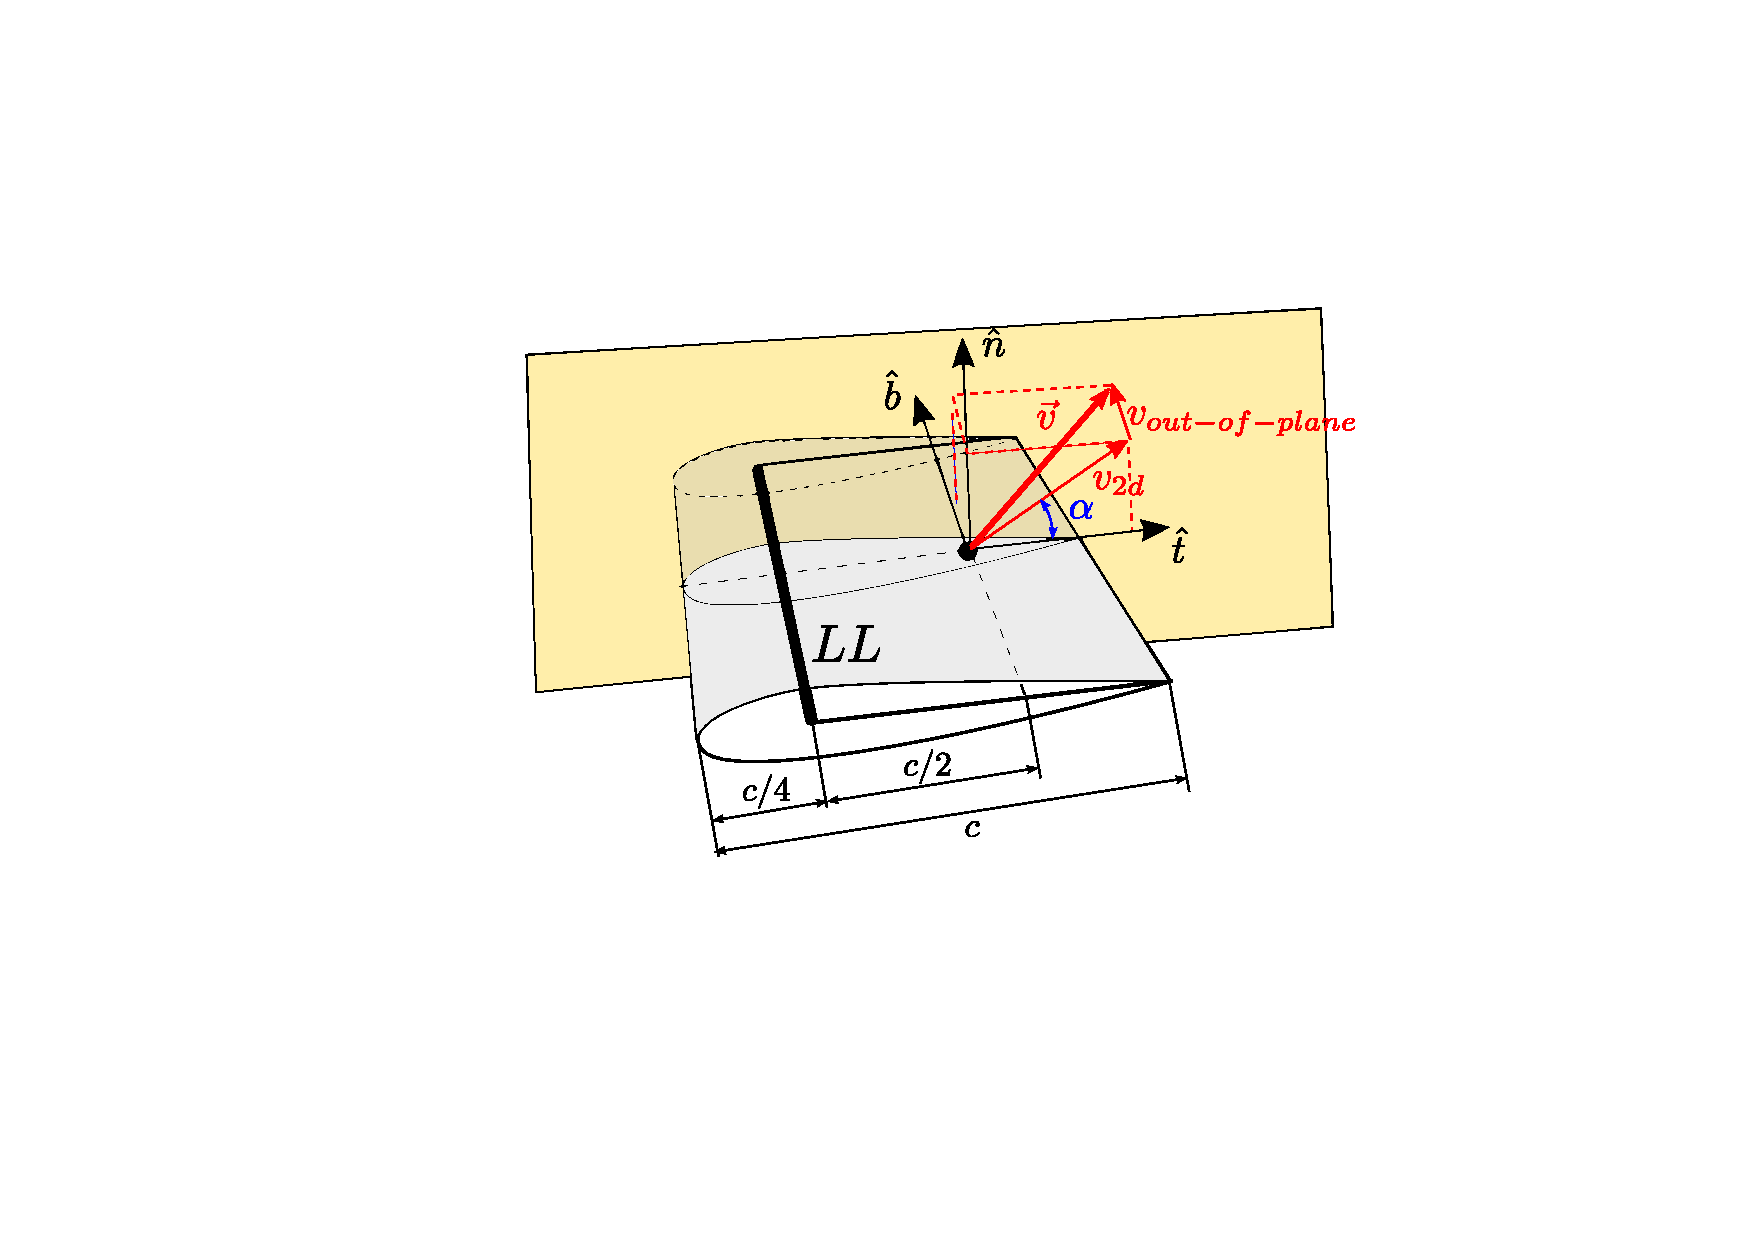
\includegraphics[width=1.0\textwidth, trim = 100 180 100 145, clip]{./images/ll_output_2} 
\caption{Lifting line data.}
\label{fig:ll_output}
\end{figure}

\subsection{Chordwise Loads} 
Chordwise loads allow to obtain the distribution of the forces, pressure and the geometrical
quantities along the chord at a specific spanwise section of a parametric component. 

Warning: at the moment, the chordwise load card is implemented only for parametric components. 

An example \param{analysis} group for chordwise loads on parametric components:

\begin{inputfile}[frame=single, caption={dust\_post.in for chordwise load 
  on parametric components}, label={file:dust_post.in_chordwise_param}]
!--- Data Names ---
data_basename = ./Output/sim_results
basename =     ./Postpro/postpro_output

analysis = {

  type = chordwise_loads
  name = cl01
  start_res = 1
  end_res = 100
  step_res = 1
  format = dat
  average = F
  
  component = wing
  n_station  = 2
  span_station = (/1., 1.5/) 
  axis_nod = (/ 0.0, 0.0, 0.0 /)
  axis_dir = (/ 0.0, 0.1, 0.0 /)

}
\end{inputfile}

\begin{itemize}
\item \param{type}: \textit{required:} one for each \param{analysis}. \textit{multiple:} no

type of the analysis, \opt{chordwise\_loads} for chordwise loads

\item \param{name}: \textit{required:} one for each \param{analysis}. \textit{multiple:} no

name of the analysis, will be appended as a suffix to \param{basename}

\item \param{start_res}: \textit{required:} one for each \param{analysis}. 
\textit{multiple:} no

First result in the time series of the solver results to analyse.

\item \param{end_res}: \textit{required:} one for each \param{analysis}. 
\textit{multiple:} no

Last result in the time series of the solver results to analyse.

\item \param{step_res}: \textit{required:} one for each \param{analysis}. 
\textit{multiple:} no

Stride to employ when loading the time series of the solver results. 

\item \param{format}: \textit{required:} one for each \param{analysis}. 
\textit{multiple:} no

format of the processed results, can be \opt{dat} for formatted ascii files 
output or \opt{tecplot} for tecplot plt files

\item \param{average}: \textit{required:} no. \textit{multiple:} no. 
\textit{default:} False

average the results in the given time span.

\item \param{component}: \textit{required:} one for each \param{analysis}. 
\textit{multiple:} no.

component (parametrically generated) to analyse. Only one component can be 
enabled for each analysis. 

\item \param{axis_nod}: \textit{required:} one for each \param{analysis}. 
\textit{multiple:} no.

Coordinates of the node from which to start the line around which to calculate 
the distribution of moment along the span.

\item \param{axis_dir}: \textit{required:} one for each \param{analysis}. 
\textit{multiple:} no.

Direction of the line (starting from \param{axis_nod}) around which to calculate 
the distribution of moment along the span.

\item \param{n\_station}: \textit{required:} no. \textit{multiple:} no. 
\textit{Default:} 1

Number of stations where the loads are extracted 

\item \param{span\_station}: \textit{required:} no. \textit{multiple:} no. 
\textit{Default:} (/0./)

Spanwise coordinates in the component reference frame (in wind axis) where they are extracted
The vector dimension must be the same as \param{n\_station}

\end{itemize}

\subsubsection{Output .dat file}

The output file containing chordwise loads in \param{.dat} format has 
the following structure. The first line is a header specifying the 
structural component. As an example,
\begin{inputfile}[frame=single]
  1: # Chordwise load of component: wing
\end{inputfile}
The second line contains the spanwise location and the chord length evaluated at the first requested
time step \param{start\_res}.  
\begin{inputfile}[frame=single]
  2: # spanwise_location:    1.00; chord_length:  0.40     
\end{inputfile}
The third line contains the number of chordwise section \param{n\_chord} in which the 
structural component is divided and the number of time steps \param{n\_time}
of the analysis. As an example, the output file for a 10-section blade reads
\begin{inputfile}[frame=single]
 3: # n_sec : 10 ; n_time : 100. Next lines: x_chord , z_chord
\end{inputfile}
The third line also introduce the content of lines 4 and 5. Line 4 contains 
the chordwise coordinate \param{x\_chord} of the centre of the panels, 
line 4 contains the thickness dimension \param{z\_chord} of the profile, taken at \param{start\_res}.
As an example, if the the chord length is 0.4 and it is divided in 10 uniform sections with chord 0.05, 
the output file reads
\begin{inputfile}[frame=single]
 3:  0.130E+000  0.900E-001  0.500E-001 ...
 4: -0.257E-002 -0.711E-002 -0.103E-001 ...
\end{inputfile}
The fifth line is another header file containing the fields and their 
dimension collected in the next \param{n\_time} lines.
\begin{inputfile}[frame=single]
  6: # t, n\_chord
\end{inputfile}
The first field is the time. The chordwise loads of the \param{n\_chord} 
sections follow. 

The files generated by sectional loads contain, as sectional quantity:
\begin{itemize}
  \item \texttt{Pres}: Panel pressure for 3D panels, or delta pressure for vortex lattice or 
                      lifting  line. 
  \item \texttt{Cp}: Panel pressure coefficient for 3D panels, or delta pressure 
                    coefficent for vortex lattice or lifting line. The implemented formulation is 
                    \begin{equation}
                      C_p = \dfrac{P - P_\infty}{\dfrac{1}{2} \rho_\infty U_\infty^2}
                    \end{equation}
                    Where $P_\infty$ is equal to \param{P\_inf}, $\rho_\infty$ is equal to \param{rho\_inf} and 
                    and $U_\infty$ is equal to the norm of \param{u\_inf} or \param{u\_ref} if \param{u\_inf} is zero. 
  \item \texttt{dFx}: Panel force per unit length in chordwise direction
  \item \texttt{dFz}: Panel force per unit length in flapwise direction
  \item \texttt{dNx}: Panel local normal in chordwise direction
  \item \texttt{dNz}: Panel local normal in flapwise direction
  \item \texttt{dTx}: Panel local tangent in chordwise direction
  \item \texttt{dTz}: Panel local tangent in flapwise direction
  \item \texttt{x\_cen}: Panel center chordwise coordinate
  \item \texttt{z\_cen}: Panel center flapwise coordinate
\end{itemize}


\subsection{Aeroacoustics}
The aeroacoustics postprocessing is a specific analysis used to 
extract from results all the various data required to perform an 
aeroacoustics analysis (with an external software) on the analysed results. 
It is available only in .dat ascii format  and it is intended rather than 
to be directly plotted/visualized to act as input for another software.

\begin{inputfile}[frame=single, caption={dust\_post.in for aeroacoustics}, 
  label={file:dust_post.in_aeroacoustics}]
!--- Data Names ---
data_basename = ./Output/sim_results
basename =     ./Postpro/postpro_output

analysis = {

type = aeroacoustics
name = aer01
start_res = 1
end_res   = 100 
step_res  = 1
format = dat

component = wing
component = tail

}
\end{inputfile}

\begin{itemize}
\item \param{type}: \textit{required:} one for each \param{analysis}. \textit{multiple:} no

type of the analysis, \opt{aeroacoustics} for aeroacoustics data

\item \param{name}: \textit{required:} one for each \param{analysis}. \textit{multiple:} no

name of the analysis, will be appended as a suffix to \param{basename}

\item \param{start_res}: \textit{required:} one for each \param{analysis}. 
\textit{multiple:} no

First result in the time series of the solver results to analyse.

\item \param{end_res}: \textit{required:} one for each \param{analysis}. 
\textit{multiple:} no

Last result in the time series of the solver results to analyse.

\item \param{step_res}: \textit{required:} one for each \param{analysis}. 
\textit{multiple:} no

Stride to employ when loading the time series of the solver results. 

\item \param{format}: \textit{required:} one for each \param{analysis}. 
\textit{multiple:} no

format of the processed results, can only be \opt{dat} for formatted ascii 
files output in case of aeroacoustics data analysis

\item \param{component}: \textit{required:} no. \textit{multiple:} yes. 
\textit{default:} all components.

Components to include in the aeroacoustics data. Only the data of the 
selected components will be included in the output file. 

\end{itemize}


%%%%%%%%%%%%%%%%%%%%%%%%%%%%%%%%%%%%%%%%%%%%%%%%%%%%%%%%%%%%%%%%%%%%%%%%%%%%%%%%%
%% Source defintions
%%%%%%%%%%%%%%%%%%%%%%%%%%%%%%%%%%%%%%%%%%%%%%%%%%%%%%%%%%%%%%%%%%%%%%%%%%%%%%%%%
% When no use outcomment
%\bibliographystyle{alpha}

\renewcommand\bibname{References}
\bibliography{base/sources}


%%%%%%%%%%%%%%%%%%%%%%%%%%%%%%%%%%%%%%%%%%%%%%%%%%%%%%%%%%%%%%%%%%%%%%%%%%%%%%%%%
%% Inserting the appendix
%%%%%%%%%%%%%%%%%%%%%%%%%%%%%%%%%%%%%%%%%%%%%%%%%%%%%%%%%%%%%%%%%%%%%%%%%%%%%%%%%
% When no use outcomment
%\newpage
\appendix 
% Adds appendix as chapter to toc
\addcontentsline{toc}{chapter}{Appendix}


\chapter{First}


\chapter{Second}


\end{document}*/***********************************************************************8	
